%% move stuff to defs file
\newcommand{\todo}[1]{{\bfseries [[#1]]}}
%% To disable, just uncomment this line
 %%\renewcommand{\todo}[1]{\relax}

\documentclass{acm_proc_article-sp}
\usepackage{url}
\usepackage{fancyvrb}
\usepackage{alltt}
\usepackage{comment}
\begin{document}

\title{Can We Crunch the Social Graph on the Cheap?}

\numberofauthors{7}
\author{
Jacob Nelson, Brandon Myers, Andrew Hunter, Dan Grossman, Mark Oskin,
Carl Ebeling, Luis Ceze\\
University of Washington\\
\email{\{nelson, bdmyers, ahh, djg, oskin, ebelin, luisceze\}@cs.washington.edu}\\ \\
Simon Kahan \\ 
Pacific Northwest National Lab\\
\email{skahan@cs.washington.edu}\\ \\
Preston Briggs\\ 
Cray Inc.\\
\email{preston.briggs@gmail.com}\\
}

\maketitle
\begin{abstract}

 Techniques from graph analytics have found important applications in
  areas such as social networks and bioinformatics. These irregular
  problems present a challenge for parallel machines: obtaining
  performance is not straightforward. Multithreading works well for
  such problems, but the only large-scale implementation of the technique
  is the Cray XMT, an expensive, non-commodity machine.

  Our goal is to build a system with XMT-like properties, implemented
  with commodity processors. This paper presents a runtime for latency
  tolerance, along with our plans for scaling up to multiple
  nodes. Our analysis shows the feasibility of our approach.
\end{abstract}

\section{Introduction}


Techniques from graph analytics have found important applications in
areas such as social networks and bioinformatics. \todo{more!}


% In January 2011, Facebook had 500 million active users with an average
% of 130 friends each \cite{Facebook:2011p91}.
% Facebook's friend suggestion
% algorithm in 2010 ran on a 40-node cluster with 72GB memory per
% node. Even with that capacity, new suggestions could only be computed
% every two days \cite{Backstrom:2010p90}.


The most interesting computational challenge comes from large,
low-diameter, power law graphs: this combination makes extracting
performance difficult. Their size keeps them from fitting in a single
commodity machine's memory. Their low diameter means that they are
difficult to lay out with locality: every vertex needs to be near every
other vertex. Their power law distribution means that a few vertices
generate much more work than the rest, leading to computational
imbalance and even less locality. Together, these properties lead to a
difficult conclusion: each edge traversal is likely to be a very
expensive cache miss.

Multithreading is a technique that has been used successfully to
implement efficient computations for these graphs. The Cray XMT is an
example of such an approach: it solves the memory latency problem
through concurrency rather than caching. Each XMT processor supports
128 hardware contexts and 1024 outstanding memory operations, and is
able to switch contexts every cycle \todo{cite XMT description}. This ability comes at a cost: the
XMT is an expensive, non-commodity machine. \todo{don't we want to also say XMT has poor performance on x kind of apps?}


\begin{figure*}[htbp]
  \begin{center}
    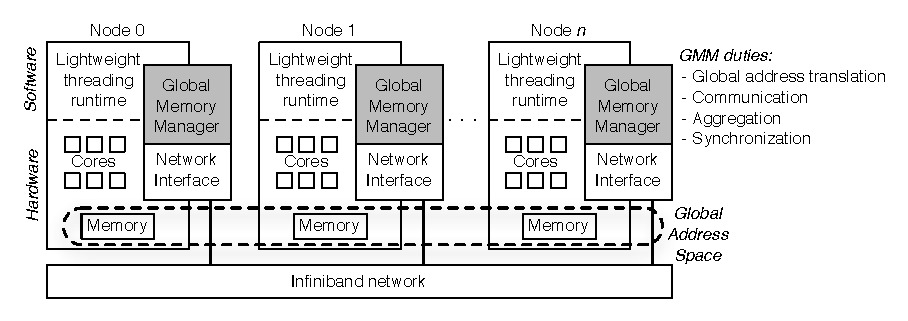
\includegraphics[width=0.9\textwidth]{figures/system-overview.pdf}
	\end{center}
	\caption{Overview of our proposed system design. The base
          system is a cluster of commodity nodes and interconnect. We
          add a latency-tolerant runtime and a global memory manager
          to obtain efficient access to the global address space. Only
          the shaded components may require hardware design.}
	\label{fig:system-overview}
\end{figure*}

We want the best of both worlds. Our goal is to build a system that
has good performance on these low-locality graph codes but is
implemented with cheap commodity processors.

Figure~\ref{fig:system-overview} shows the structure of our
proposal. It is composed of multiple nodes built with commodity
processors, communicating over an Infiniband network. We add two
components: a runtime system, responsible for executing the user's
threads, and a global memory manager, responsible for facilitating
memory requests to the non-coherent global memory shared across the
nodes.  We are exploring a mix of hardware and software
implementations of the memory manager.

This paper explores the feasibility of our multi-node goal using a
single-node implementation of our lightweight threading runtime. We
use prefetch instructions together with lightweight threads to
tolerate the latency of DRAM access on the local node node. We use
pointer chasing benchmarks to verify our runtime's overhead is
acceptable. We also model the effects of pointer chasing on a remote
node.

The rest of the paper is organized as follows. We describe our
proposal from a programmer's viewpoint in section~\ref{sec:model}. We
describe the implementation of our latency-tolerant runtime and plans
for extending to multiple nodes in section~\ref{sec:approach}. We
evaluate our runtime in section~\ref{sec:evaluation}.  We present
related work in section~\ref{sec:related} and conclude in
section~\ref{sec:conclusion}.

\section{Programming model}
\label{sec:model}

Our shared-memory programming model partitions the overall address
space into a global shared address space and per node private address
spaces.  Locality may be exploited directly by the programmer in the
node private address spaces, just as in a conventional cache-coherent
multiprocessor node.  In contrast, locality cannot be exploited in the
global space: its value is in providing high bandwidth random access
to any word in a shared data structure by any processor.

Whereas in the PGAS model coherency of global copies is implictly
maintained across the system \todo{cite pgas?}, we forego caching of globally shared
data.  A node can exploit temporal locality of data stored in
the global space only by first copying it into the node's local space.
In this way, a node can access data at random across the system while
incurring no hardware coherence overhead: consistency is enforced by
our mechanisms for explicit global synchronization.

The model promises efficiency subject to the presence of sufficient
concurrency.  Exactly how that concurrency is expressed by the
programmer is language dependent.  Our programming model serves to
augment threaded programming languages so that they become latency
tolerant on large address spaces.  Software multithreading is used to
provide latency tolerance: a computation that is about to execute a
long latency operation such as a remote memory reference initiates the
operation and then yields to the scheduler, which quickly resumes
execution of another computation.  Concurrency is also used -- via
aggregation of requests to a common node destination -- to make more
efficient use of network bandwidth and in some cases reduce bandwidth
demands.

Synchronization on locations in the node private address space is the
same as on conventional systems.  Synchronization on global addresses
works differently: we provide atomic operations such as {\tt
  int\_fetch\_add} as well as operations using full-bits, as on the
Cray XMT.  As is true for other long latency operations,
synchronization latency is tolerated by yielding to the scheduler.
Even non-blocking global atomics yield: atomic operations executed as
x86 instructions sabbotage concurrency by forcing all outstanding
memory references to complete before new ones can be issued.  By
yielding, the core can switch to another computation while the
synchronization is accomplished outside of the pipeline.  In addition,
the implementation can exploit aggregation when concurrency is
abundant to increase the throughput of global synchronization.

Thus, the programming model provides the programmer with options: express
locality within the private space, and it will be exploited to reduce
latency and bandwidth \todo{exploited by what? by the exisiting locality hardware like cache hierarchy?}; express concurrency, and it will be used toward
tolerating latency and reducing the cost of bandwidth.

\begin {comment}
\todo{Change to discuss API:

context switches:
  yield()
  discuss coroutines

mem:
  alloc()
  read(p) 
  write(p, d)
  prefetch(p)

sync:
 {read, write} {EE, EF, FE, FF}
}

While the ideal programming model is one that facilitates easy
expression in the problem domain as well as efficient execution on the
available hardware, our programming model today is motivated by only
efficient execution: it exists as a rudimentary library for concept
demonstration, not as a language suitable for development.  The
programming model we use today is therefore only partially formed. It
exists as an augmentation of existing threaded programming models such
as pthreads or openmp that are readily available on most computer
systems.

Though not strictly necessary, for ease of exposition we imagine a
one-to-one binding between threads and cores.  Our model manifests
within any thread independently of the others as a ``fray'' \todo{for lack
of better term }.  Within the thread, a fray instance is the
instantiation of a set of coroutines and a scheduler.  Instantiation
is at user-level and the operating system sees the entire fray as as a
single user-level thread.

\todo{ describe calls that perform thread \& scheduler instantiation; and schedule activation }

Each coroutine executes non-preemptively \todo{seems like non-premptively isn't ``how" it executes, rather how it is scheduled, maybe say ``cooperatively"?}, utilizing the core to which
its ``parent'' thread has been assigned by the operating system until it
reaches a yield point.  Typically, the coroutine yields after
initiating a prefetch operation on data that the programmer or
compiler anticipates would probably not complete before the data is
referenced by a subsequent load operation.  In this way, the core
continues to execute instructions for other coroutines when otherwise
it would likely stall.  The programming model thus tolerates latency.

\todo{ describe calls to prefetch-and-yield }

When a thread frays, for the sake of expediency, a fixed portion of
its stack is divided amongst the coroutines.  Given a finite stack,
each coroutine is constrained to execute a call tree of depth known to
be finite at compilation time: recursion is not yet permitted.

\todo{ discussion of coroutines \& synchronization } Were a coroutine to
block on a synchronization variable shared with other threads, the
entire fray would suspend execution.  This can lead to deadlock when,
for example, one coroutine waits to consume from another thread that
is waiting to consume what only another coroutine in this first fray
can produce.  Instead, coroutines must yield on failed synchronization
events, spinning rather than blocking, where were they bona fide
threads, blocking might be more efficient.

\todo{ say something about ``synchronization'' within a fray }

Coroutines completing their work yield without adding themselves to
the scheduling queue.  The last coroutine to exit in this way returns
as the main thread, as in the common  fork-join model of parallelism.

\end{comment}

\section{Implementation}
\label{sec:approach}


The goal of our implementation is to use multithreading to tolerate
the latency of random accesses to memory in a global address space
spread across multiple nodes. This goal has three key challenges:

\begin{itemize}
\item {\bf Lightweight multithreading}

  We expect to need hundreds of
  threads to tolerated a cluster's network latency, so our threading
  implementation must have low overhead.
  
\item {\bf Concurrency in global memory references}

  A thread making a long-latency global memory reference must be able
  to yield and allow other threads to make progress.

\item {\bf Low overhead synchronization}

  In a system with high degrees of concurrency, lightweight
  synchronization primitives are important.
\end{itemize}

We discuss our approach to solving each of these challenges in
turn. For each one, we discuss both our current single-node
implementation and ideas for a multi-node implementation.

\subsection{Lightweight multithreading}

Our approach to supporting many lightweight threads uses a cooperative,
user-level multitasking system built using coroutines.

There are three main concerns in designing the coroutine
mechanism. First, the working set of each coroutine must be small, so
many coroutines can be active without trashing the cache. Second,
context switches must be fast, so that overhead does not swamp actual
work. Third, when a coroutine yields, we must choose a suitable
coroutine to run next.

We minimize context size by treating context switches as function
calls, as in~\cite{charm}. This allows us to save and restore the
minimum number of registers allowed by the ABI, and depend on the
compiler to save and restore any other registers in use. We minimize
context switch time both by keeping contexts small and by doing all
switching and scheduling in user space, as in \todo{cite other green
  threads packages, like qthreads}.

There are a number of possibilites for coroutine scheduling.
Ideally, a thread would be rescheduled when its request had
completed, but this may complicate the scheduling decision and slow
down context switches. A simple round-robin scheduler may be sufficient.

\subsubsection{Single-node implementation}
We implemented coroutines as described, with a round-robin
scheduler. If a prefetched data value is no longer in the cache when
the coroutine is rescheduled and the value is used, the coroutine pays
the full cost of the fetch.

\subsubsection{Multi-node ideas}
We will explore how the memory manager and coroutine scheduler may
interact, so that threads waiting on long-latency memory operations or
synchronization operations will be scheduled soon after their
operations have completed. 

\subsection{Concurrency in global memory references}

To enable concurrency in memory references, we break each read or
write into two operations: the {\em issue} operation and the {\em
  complete} operation. The read issue operation starts data moving
towards the processor and returns immediately, like a prefetch; the
read complete operation blocks until data is available. The write
issue operation takes data along with an address, and starts an
asynchronous write; the write complete operation blocks until the
write is committed.

A read operation in user code consists of three steps: a {\em read
  issue}, which causes the data to start moving; a {\em yield}, which
causes another thread to start executing, overlapping the read
latency; and, once the reading thread has been rescheduled, a {\em
  read complete} blocks until the data is available. A write operation
follow the same pattern.

\subsubsection{Single-node implementation}
We use prefetch instructions for the issue operation, and regular
blocking reads and writes for the complete operation. Since we expect
these global references to have low locality, we use the
``non-temporal'' form of prefetch, which tries to bring the data near
the core without disturbing the state of the cache
hierarchy \cite{intel:swdev}.

\subsubsection{Multi-node ideas}

We believe we will need hundreds of outstanding memory references per processor to
cover the latency of remote references in a multi-node
system\todo{ can we make a stronger statement? we know it will be 300$+$ according to our calculations}. Unfortunately, commodity processors have much smaller limits
on memory concurrency: section~\ref{subsubsec:evalsinglebase} finds a limit of
36 concurrent loads. We will have to manage memory concurrency on our
own to avoid this limit. We describe approaches in both software and
hardware.

One approach is for user code to delegate global references to a
special {\em global memory manager thread}, running on another core in
the chip. This thread translates the global address into a network
destination, makes the request through the network card to the remote
node, checks for completion, and delivers the returned data to the
requesting thread. On the remote node, the remote memory manager
thread would perform the memory operation and return the data to the
requesting node.

This approach has the benefit of enabling our entire system to be
build using commodity parts, but its potential for performance is not
clear. We have increased the overhead of a single memory operation:
what in the single node case was a simple read, is now multiple
queuing operations between threads and multiple reads and writes over
the processor's link to the network interface.

Another approach moves the global memory management to a hardware
device. We can add a coprocessor FPGA in a processor socket, listening
to coherence messages on the bus. Note that this accelerator is only a
memory proxy, not a compute coprocessor. When it detects a reference
to memory stored on a remote node, the accelerator would issue the
request through the network controller and track its progress,
delivering the data to the requesting thread when it was ready.

All global shared memory would be mapped into a segment of the local
address space on each node. The accelerator would do the
address-to-node translation. In addition, to support the issue and
complete operations for concurrency support, commands would be encoded
in the upper bits of the address: then each remote word would have multiple
addresses on the local node. Reading from the {\em issue} address would
immediately return a dummy value, but the accelerator would issue the
request over the network. Reading from the {\em complete} address
would block until the data was available.\todo{adjust with carl's suggestions}

With either approach, the question of request aggregation will be
important. Each memory request we make is small: 8 bytes is a likely
size. But most networks are optimized for bulk transfers of a few
thousand bytes. To improve network utilization, we will explore the
aggregation of multiple memory operations to different addresses on
the same remote node. 


\subsection{Low-overhead synchronization}

Just as with reads and writes, we enable concurrency around
synchronization operations by splitting them into {\em issue} and {\em
  complete} phases.

Implementing full-empty bit support efficiently on a platform not
designed for them is a challenge. It is possible to support full-empty
bit synchronization on arbitrary words by allocating additional
storage for the full-empty bits, and translating each atomic
full-empty operation into a sequence of memory operations that modify
the data and full-empty bit atomically, but this may have high
overhead. \todo{cite qthreads somehow}

One potential optimization is to limit full-empty synchronization to
pointers to aligned data types, and reuse wasted space in the
low-order bits of the pointer for full-empty bit storage. These bits
would be masked out when the pointer was returned to the user.  This
allows us to synchronize any data type through one level of
indirection.

\subsubsection{Single-node system}
Just as with reads and writes, we prefetch and yield before performing
a synchronization operation. We support only the synchronization
operations supported by our development platform; we have not
implemented full-empty bits.

\subsubsection{Multi-node ideas}

Synchronization operations can also be delegated to a memory manager
thread or accelerator. This may simplify the implementation of
synchronization operations: if only a single core (or single
accelerator) is accessing the data being synchronized, the use of
memory fences may be reduced or eliminated.

Note that we are not advocating using an FPGA as a memory controller
with attached DRAM and additional storage for full-empty bits. We
believe this unnecessarily complicates the design for such a
component. Our goal is to minimize the amount of hardware design our
proposal requires.

% 2TB global memory => 68GB of distributed FE bits.  This seems reasonable, given that a 2TB system might have 64 nodes, so ~1GB per memory manager if one manager per node.

\section{Evaluation}
\label{sec:evaluation}

Our goal is to evaluate the feasibility of our proposed runtime. We want to determine two things: whether coroutines can generate memory concurrency without incurring minimal performance overhead, and whether the system can support the level of concurrency required to tolerate the latency that will be present in a multi-node system.

We focus the evaluation on one component of the runtime: lightweight context switching. We ran pointer-chasing benchmarks on a single-node implementation of our runtime. These pointer chasing experiments are intended to model a particular ``worst-case'' behavior of irregular applications, where each memory reference causes a cache miss.

We ran these experiments on a Dell PowerEdge R410 with two Xeon X5650 (Nehalem microarchitecture)
chips and 24GB of RAM, with hyperthreading disabled. These
chips use a NUMA memory architecture, where each chip has
its own integrated memory controller and DIMMs; references to other
chips' memory are carried over Intel's cache-coherent QuickPath
Interconnect (QPI).

Our evaulation consists of two parts. First, we demonstrate that the runtime system can achieve the same performance as when there is explicit memory concurrency available: we measure pointer chasing performance and
the effects of cache pressure due to the number of contexts required. Second, we look at the runtime within the multi-node picture and simulate the effects of fetching memory over a network to show that the runtime can reach the level of concurrency required to hide the latency. In each part we begin by studying relevant aspects of our test machine's memory system so we can interpret our runtime results.


\subsection{Single-node}

We first characterize the performance of our test machine's memory
system. Then we use these results to evaluate the performance of our runtime within a single node.

\subsubsection{Base memory system performance}
\label{subsubsec:evalsinglebase}
\todo{title might be improved}

We measured two parameters: the maximum random reference
rate that can be issued by the cores in one chip and the maximum random
reference rate that can be serviced by one chip's memory controller.\todo{The 360M  "serviced" number could perhaps be an "aside" kind of paragraph since not supporting a major point}

To find the maximum random reference rate that one chip's cores
can issue, we ran pointer chasing code following the model of
Figure~\ref{fig:code}a. Each core issues $n$ list traversals
in a loop; we call $n * \textit{number of cores}$ the number of
{\em concurrent offered references}, since the memory system may not
be able to satisfy them all in parallel. Since our goal is to find a
baseline for evaluating our coroutine library, we depend on the
cores' exploitation of ILP for memory concurrency, rather than our coroutine
library.

\begin{figure*}[ht]
%list walk ILP
\begin{minipage}[b]{0.3\linewidth}
\centering
\begin{alltt}
  while (count-- > 0) \{
    list1 = list1->next;
    list2 = list2->next;
    \ldots
    list\(n\) = list\(n\)->next;
  \}
  \center{{\bf (a)}}
\end{alltt}
%\caption{Pseudocode for pointer chasing without coroutines.}
\label{fig:pointernocoro}
\end{minipage}
%listwalk green threads
\begin{minipage}[b]{0.35\linewidth}
\centering
\begin{alltt}
  while (count-- > 0) \{
     prefetch(&(list1->next));
     switch();
     list1 = read(&(list1->next));
 \}
  \center{{\bf (b)}}
\end{alltt}
  %%n lists
  % while (count-- > 0) \{
  % prefetch(&(list1->next));
  %   prefetch(&(list2->next));
   %  \ldots
   %  prefetch(&(list\(n\)->next));
   %  switch();
   %  list1 = read(&(list1->next));
   %  list2 = read(&(list2->next));
   %  \ldots
   %  list\(n\) = read(&(list\(n\)->next));
%\caption{Pseudocode for pointer chasing using coroutines.}
\label{fig:pointercoro}
\end{minipage}
%cache pressure
\begin{minipage}[b]{0.32\linewidth}
\centering
\begin{alltt}
  while (count-- > 0) \{
    prefetch(&(list1->next));
    switch();
    list1 = read(&(list1->next));
    for( i in 1 to num_local_updates ) \{
      local->data++;
      local = local->next;
   \}
  \}
   \center{{\bf (c)}}
\end{alltt}
%\caption{Pseudocode for pointer chasing with local updates.}
\label{fig:pointerupdate}
\end{minipage}
\caption{Pseudocode for: (a) pointer chasing without coroutines, (b) pointer chasing using coroutines, (c) pointer chasing with local updates. Coroutine code, as in (b), might also include ILP like what (a) depends on for memory concurrency, e.g., by doing multiple prefetches to independent lists, switch, then multiple reads.}
\label{fig:code}
\end{figure*}


The lists were sized to exceed the last level cache and were laid out
randomly with pointers spaced at a cache line granularity, maximizing
the probability of each reference being a miss. We allocated the lists
on 1GB huge pages to minimize TLB refill overhead. The lists were
allocated in the memory attached to the processor containing the cores
doing the traversal. We ran 10 traversals, measuring average rate in each, and recorded the maximum rate.


\begin{figure}[h]
	\begin{center}
		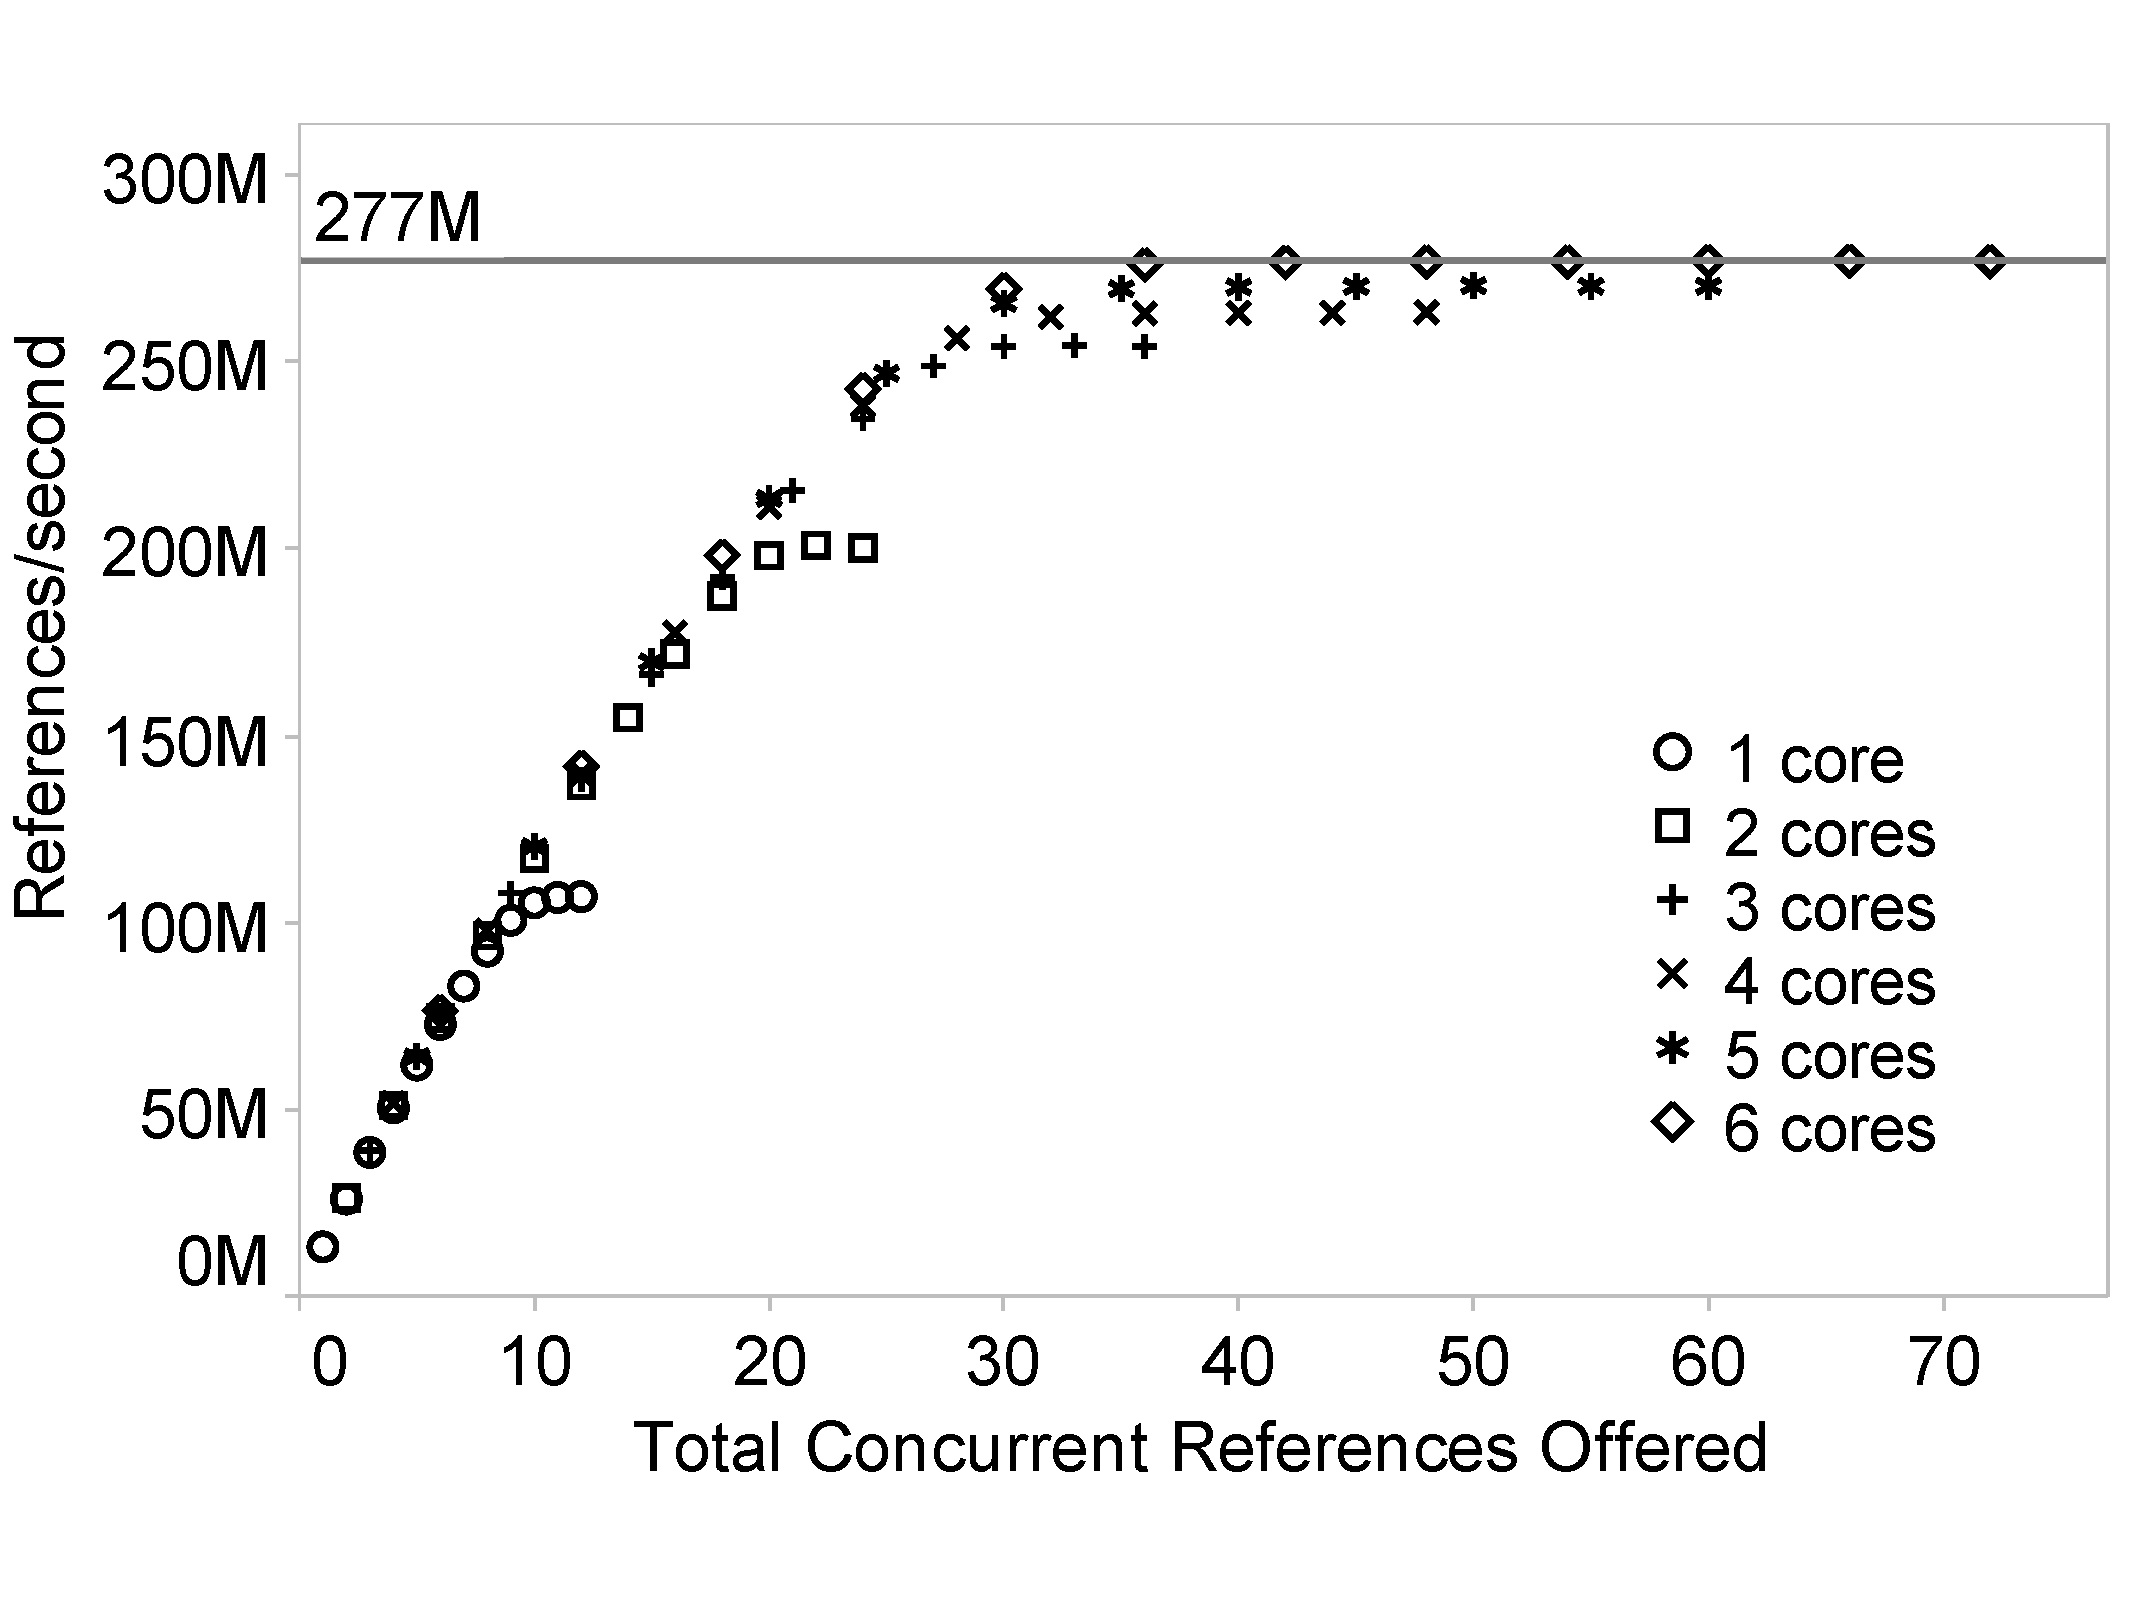
\includegraphics[width=0.5\textwidth]{figures/multi-listwalk-totalconc-edited.pdf}
	\end{center}
	\caption{Throughput of listwalk versus total number of
          concurrent references offered by the cores. Data points for
          running 1 core are shown as circles, and data points for
          running 6 cores are shown as diamonds. 
%Notice that the throughput for a single core levels out at 10
%concurrent references. For 4 to 6 cores, the throughput levels off at
%around 36 references, which seems to be the most memory concurrency a
%processor can handle.
        }
	\label{fig:listwalk-totalconc}
\end{figure}

Figure~\ref{fig:listwalk-totalconc} shows the result. Each point represents
the maximum rate pointers are traversed for a given number of
concurrent offered references. We see a maximum rate of 277 million
references per second, which agrees with the measurements found by \cite{Mandal:2010} with a similar machine. This rate is achieved when the number of offered references is 36. Note that a single core cannot support this level of
memory concurrency; the maximum reference rate for a single core is
107M. We believe this limit is due to the core's limited number of {\em line fill
  buffers} \cite{nehalem:arch}, which limits the core to 10
concurrent private cache misses.

The memory controller in the chip has more bandwidth than its
cores can saturate. To measure the memory controller's maximum random
reference rate, we extended the previous experiment so that cores in
both processors were traversing lists allocated in the first processor's
memory. With this configuration, we observed a maximum rate of 360
million references per second. We believe this difference is due to
the configuration of the processor's {\em Global Queue} \cite{nehalem:perf}, which limits the number of concurrently-executing read misses from a chips cores to its local last-level cache and memory to 32.


\subsubsection{Runtime performance}

To evaluate the performance of our runtime, we investigated two
effects: the maximum reference rate using coroutines
to obtain memory concurrency and the effects of cache pressure from the
coroutines' context storage. 

To find the maximum reference rate obtainable using our coroutine
library, we modified our pointer chasing benchmark as shown in
Figure~\ref{fig:code}b. Recall that the baseline code in Figure~\ref{fig:code}a relied solely on ILP to achieve memory concurrency, which may not be abundant in real applications. Using coroutines, there are two sources of offered
concurrent references: the ILP exploited by the processor, and the
memory concurrency enabled by prefetching and switching to a new
coroutine. As with our first experiment, we allocated the lists in the
same processor as the cores doing the traversal. 

\begin{figure}[h]
  \begin{center}
    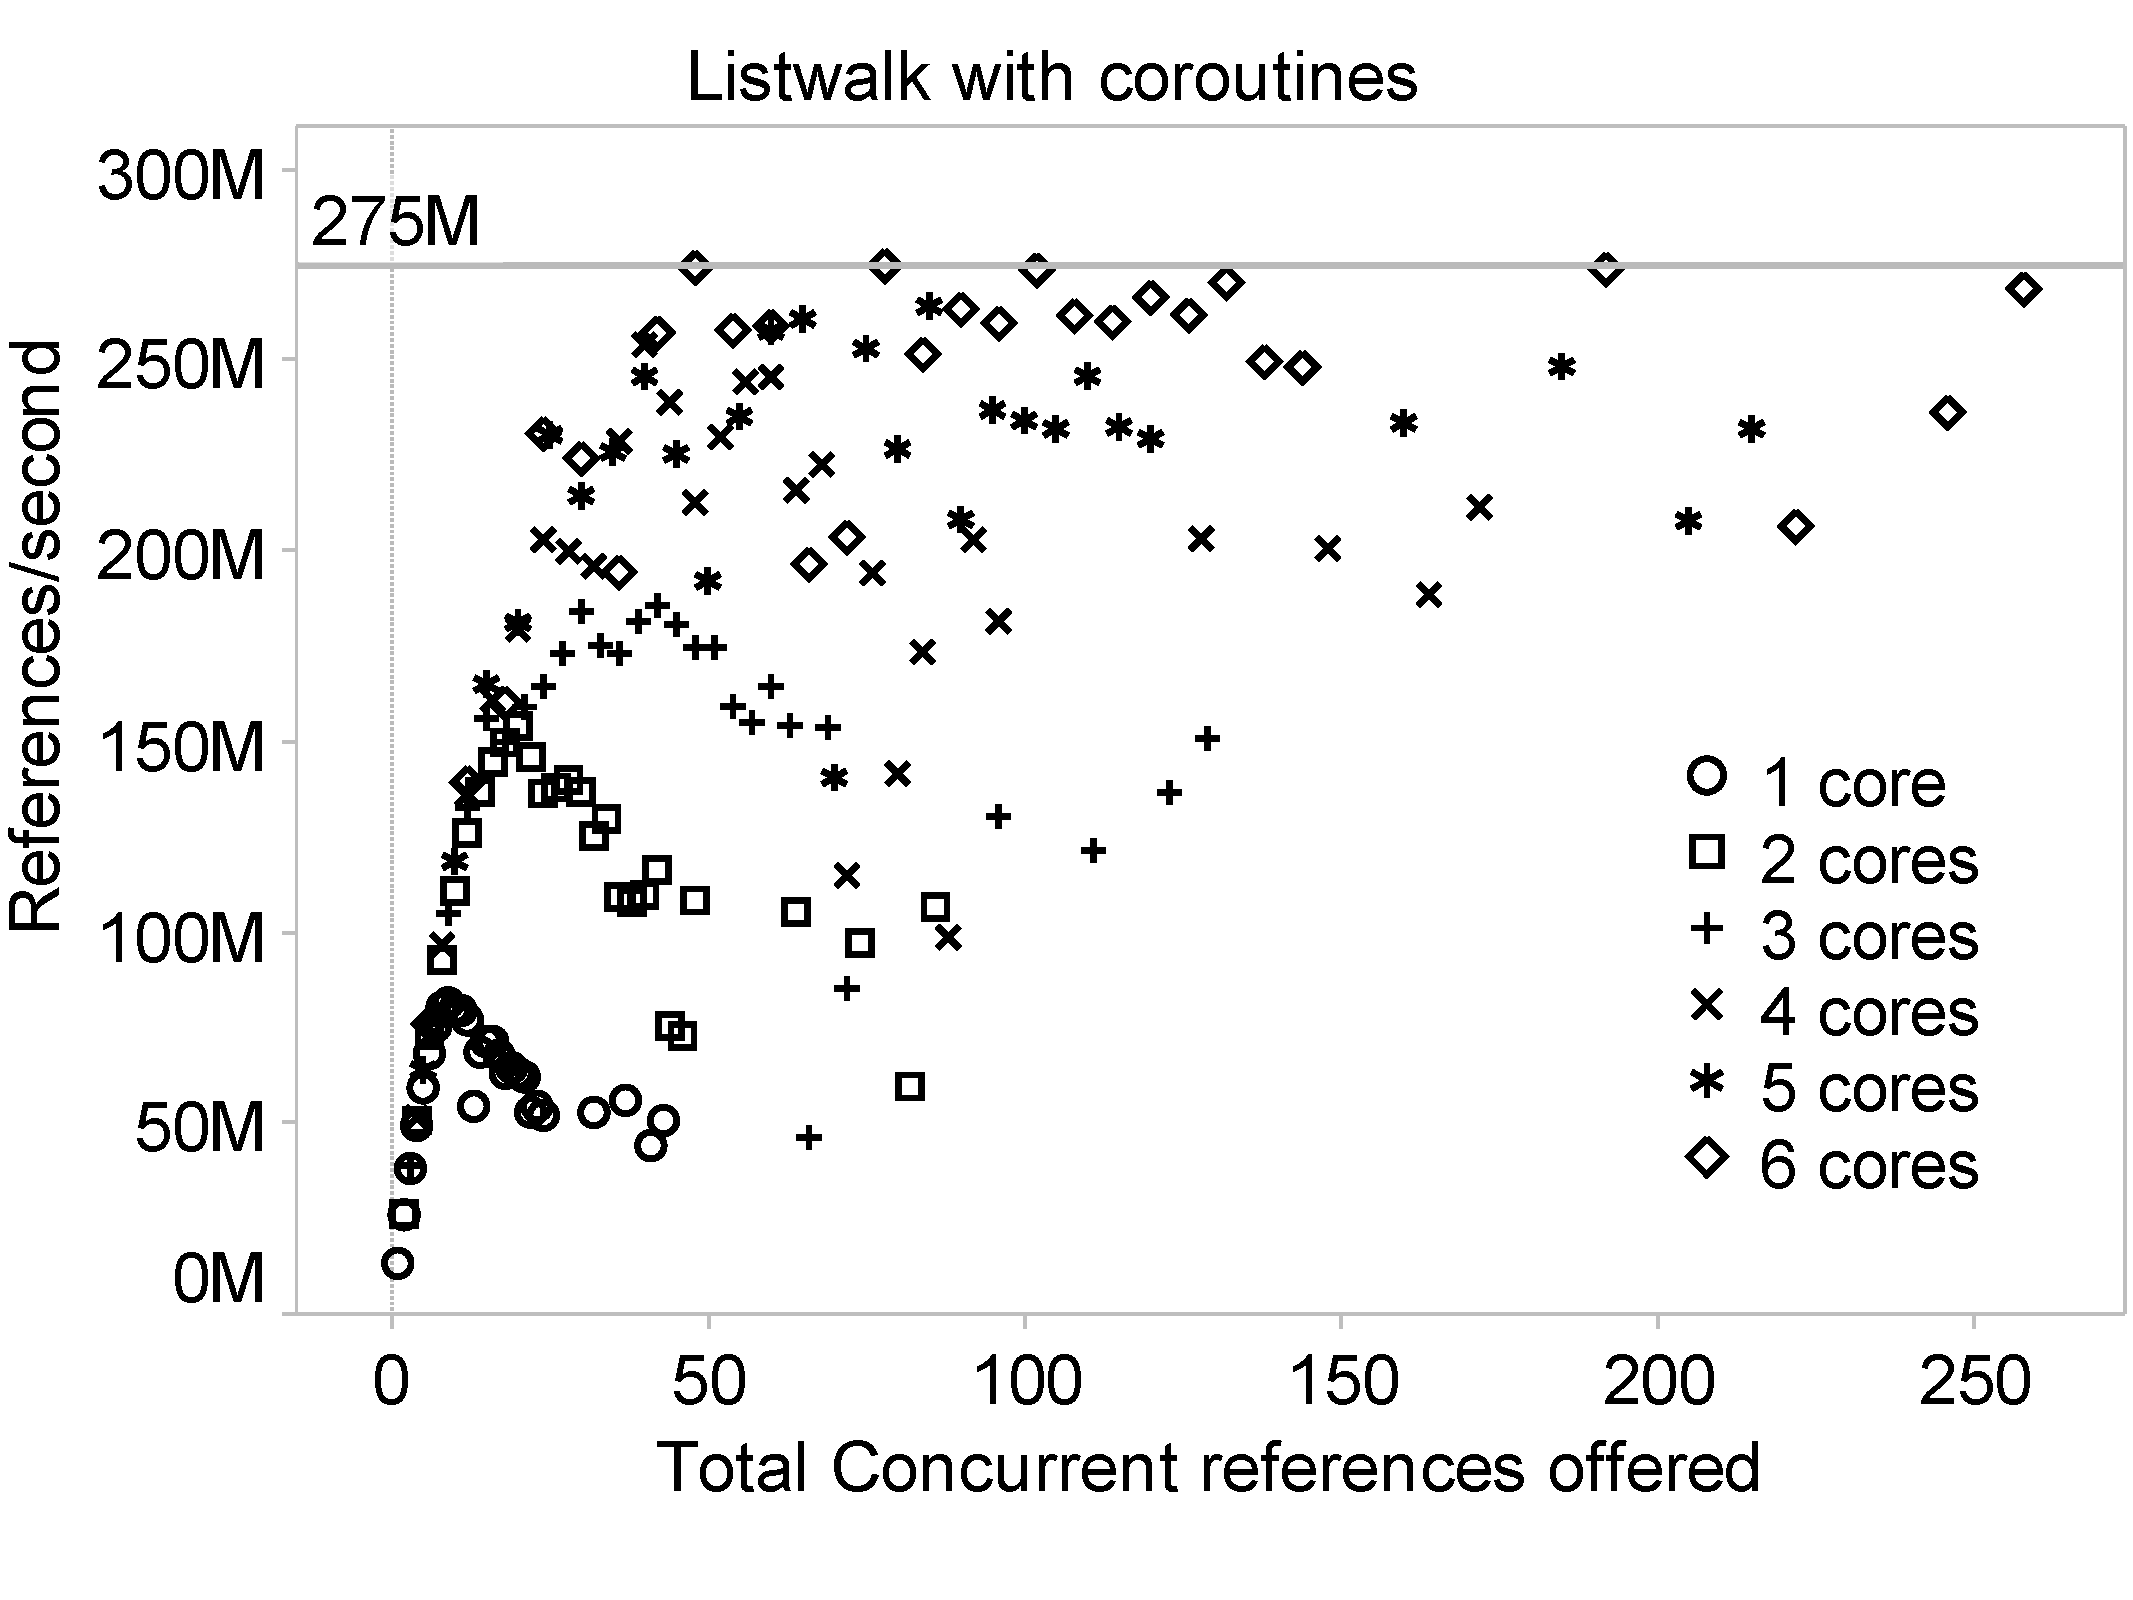
\includegraphics[width=0.5\textwidth]{figures/multi-green-edited.pdf}
  \end{center}
  \caption{Pointer chasing with coroutines, with one reference per
    coroutine. Number of coroutines per core is $\textit{total concurrent references} / \textit{number of cores}$.}
  \label{fig:multi-green}
\end{figure}

Figure~\ref{fig:multi-green} shows the result. For this
experiment, we limited memory concurrency to one concurrent miss per
coroutine, so the only source of memory concurrency is the use of
coroutines. We are able to obtain a rate of 275 million references per
second with 48 concurrent misses, or 8 coroutines per core. These
results are very close to the ILP-only experiment, but more concurrent requests are required--about 48 versus 36. When the number of references per coroutine is larger than 1, fewer coroutines are required to reach full performance.

We observe a gradual decrease in reference rate once the number of
concurrent references per core exceeds 10; we believe this is due to
later prefetches squashing earlier ones in the line fill buffers. We
also observe some points that do not follow the trend and look like noise, but these results are actually repeatable. This effect is harder to explain, but we suspect it is
due to resource contention in the cores' pipelines once the memory
system is full of requests.

%Such points are repeatably lower, and looks like the std dev of such points (the diamond ones than are low) is also higher than other "normal" points: around 35M versus 13M or less, which seems to suggest a weird effect at those numbers}


The stacks for the coroutines are stored in the data cache, where they
will compete for space with an application's data. To characterize the
effects of this cache pressure, we modified our list chasing benchmark
to include random updates to a per-coroutine local data structure that
is small enough to fit in cache. Figure~\ref{fig:code}c shows the
general idea.


\begin{figure}[h]
  \begin{center}
    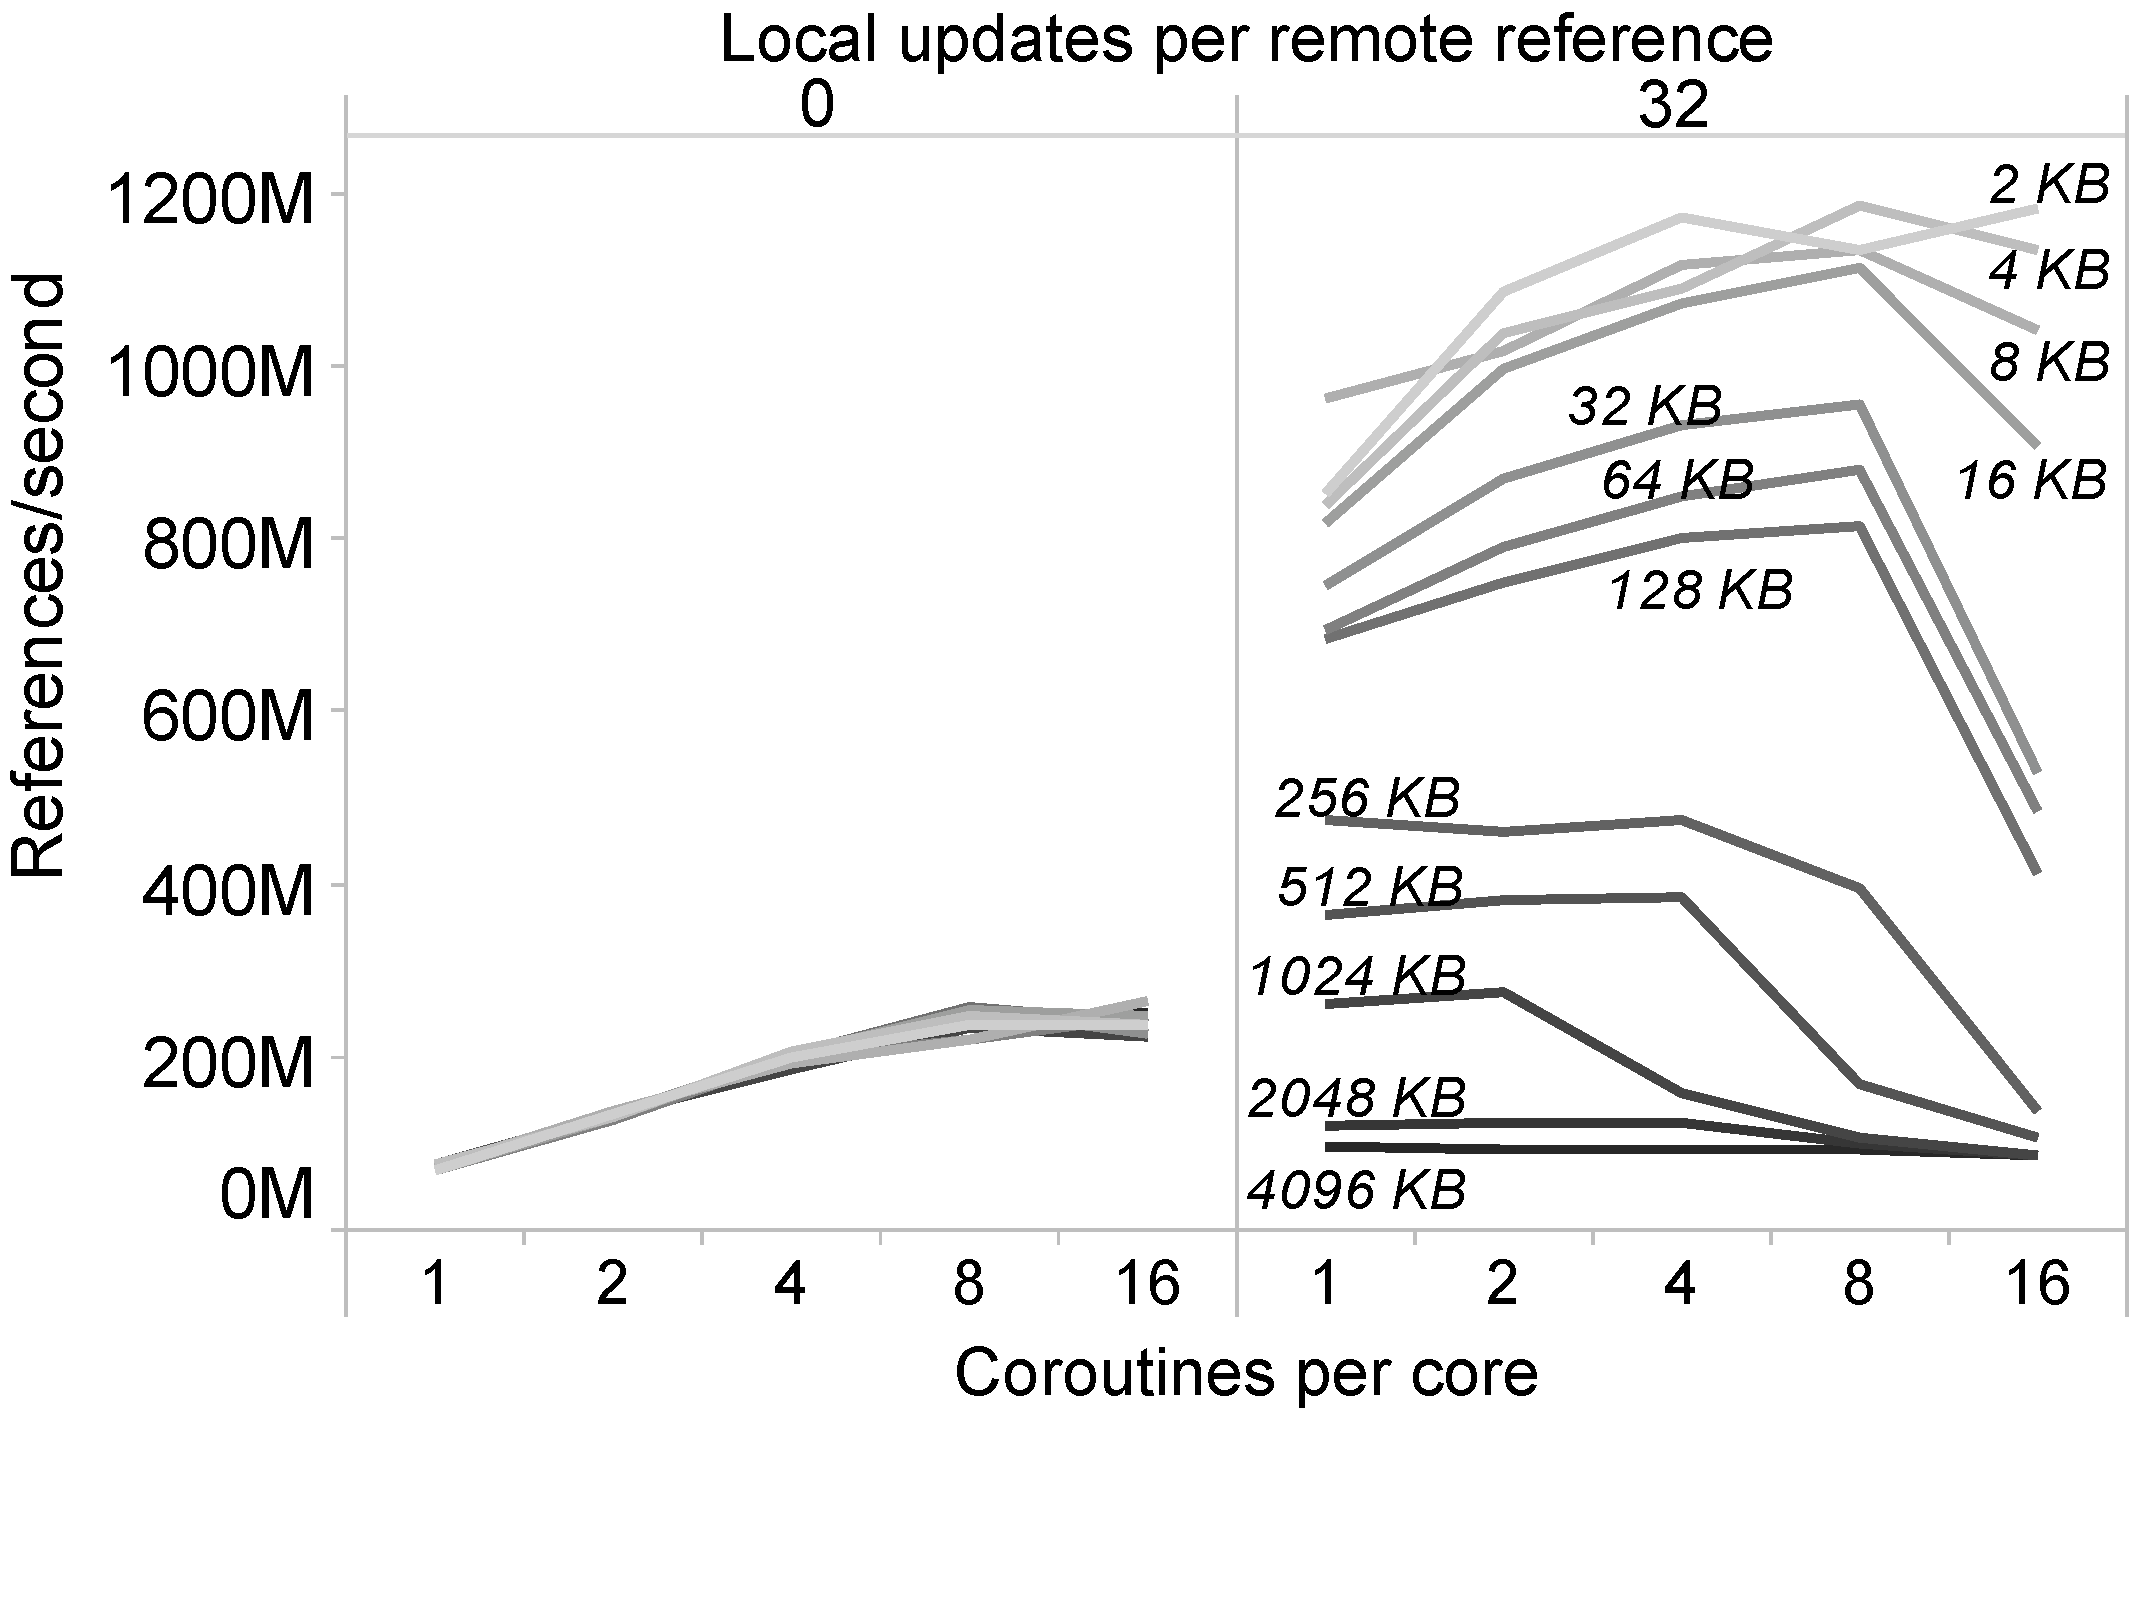
\includegraphics[width=0.5\textwidth]{figures/cache-pressure-edited.pdf}
  \end{center}
  \caption{Cache pressure with coroutines.}
  \label{fig:cache-pressure}
\end{figure}

We ran this code on six cores with all data allocated in the same
processor's memory. We varied the size of the local working set from 2KB
to 4MB, and ran both 0 and 32 local updates for each pointer
traversal. We measured the overall reference rate, including both the local updates and remote references.

Figure~\ref{fig:cache-pressure} shows the result. On the left of the
figure, we see the list-traversal-only case, where we allocate
per-coroutine space but make no references to it. As we would expect,
the reference rates grow with the number of coroutines just as in
Figure~\ref{fig:multi-green}. On the right of the figure, we see the
case with 32 updates for each list traversal. While performance
decreases for large working set sizes and large number of coroutines,
we see speedup as number coroutines increases for up to 128KB working set size with 8 coroutines per
core.

\subsection{Multi-node}

To evaluate the potential for our runtime to perform in the multi-node case, we simulated a network delay and saw whether the runtime could tolerate the larger latency. First we measure the QPI bandwidth between the two chips of the test machine, since the chip would talk to the network interface over a QPI link.

% take this figure out if we need the space
% the main point is room for remote references to local memory
\begin{figure}[h]
  \begin{center}
    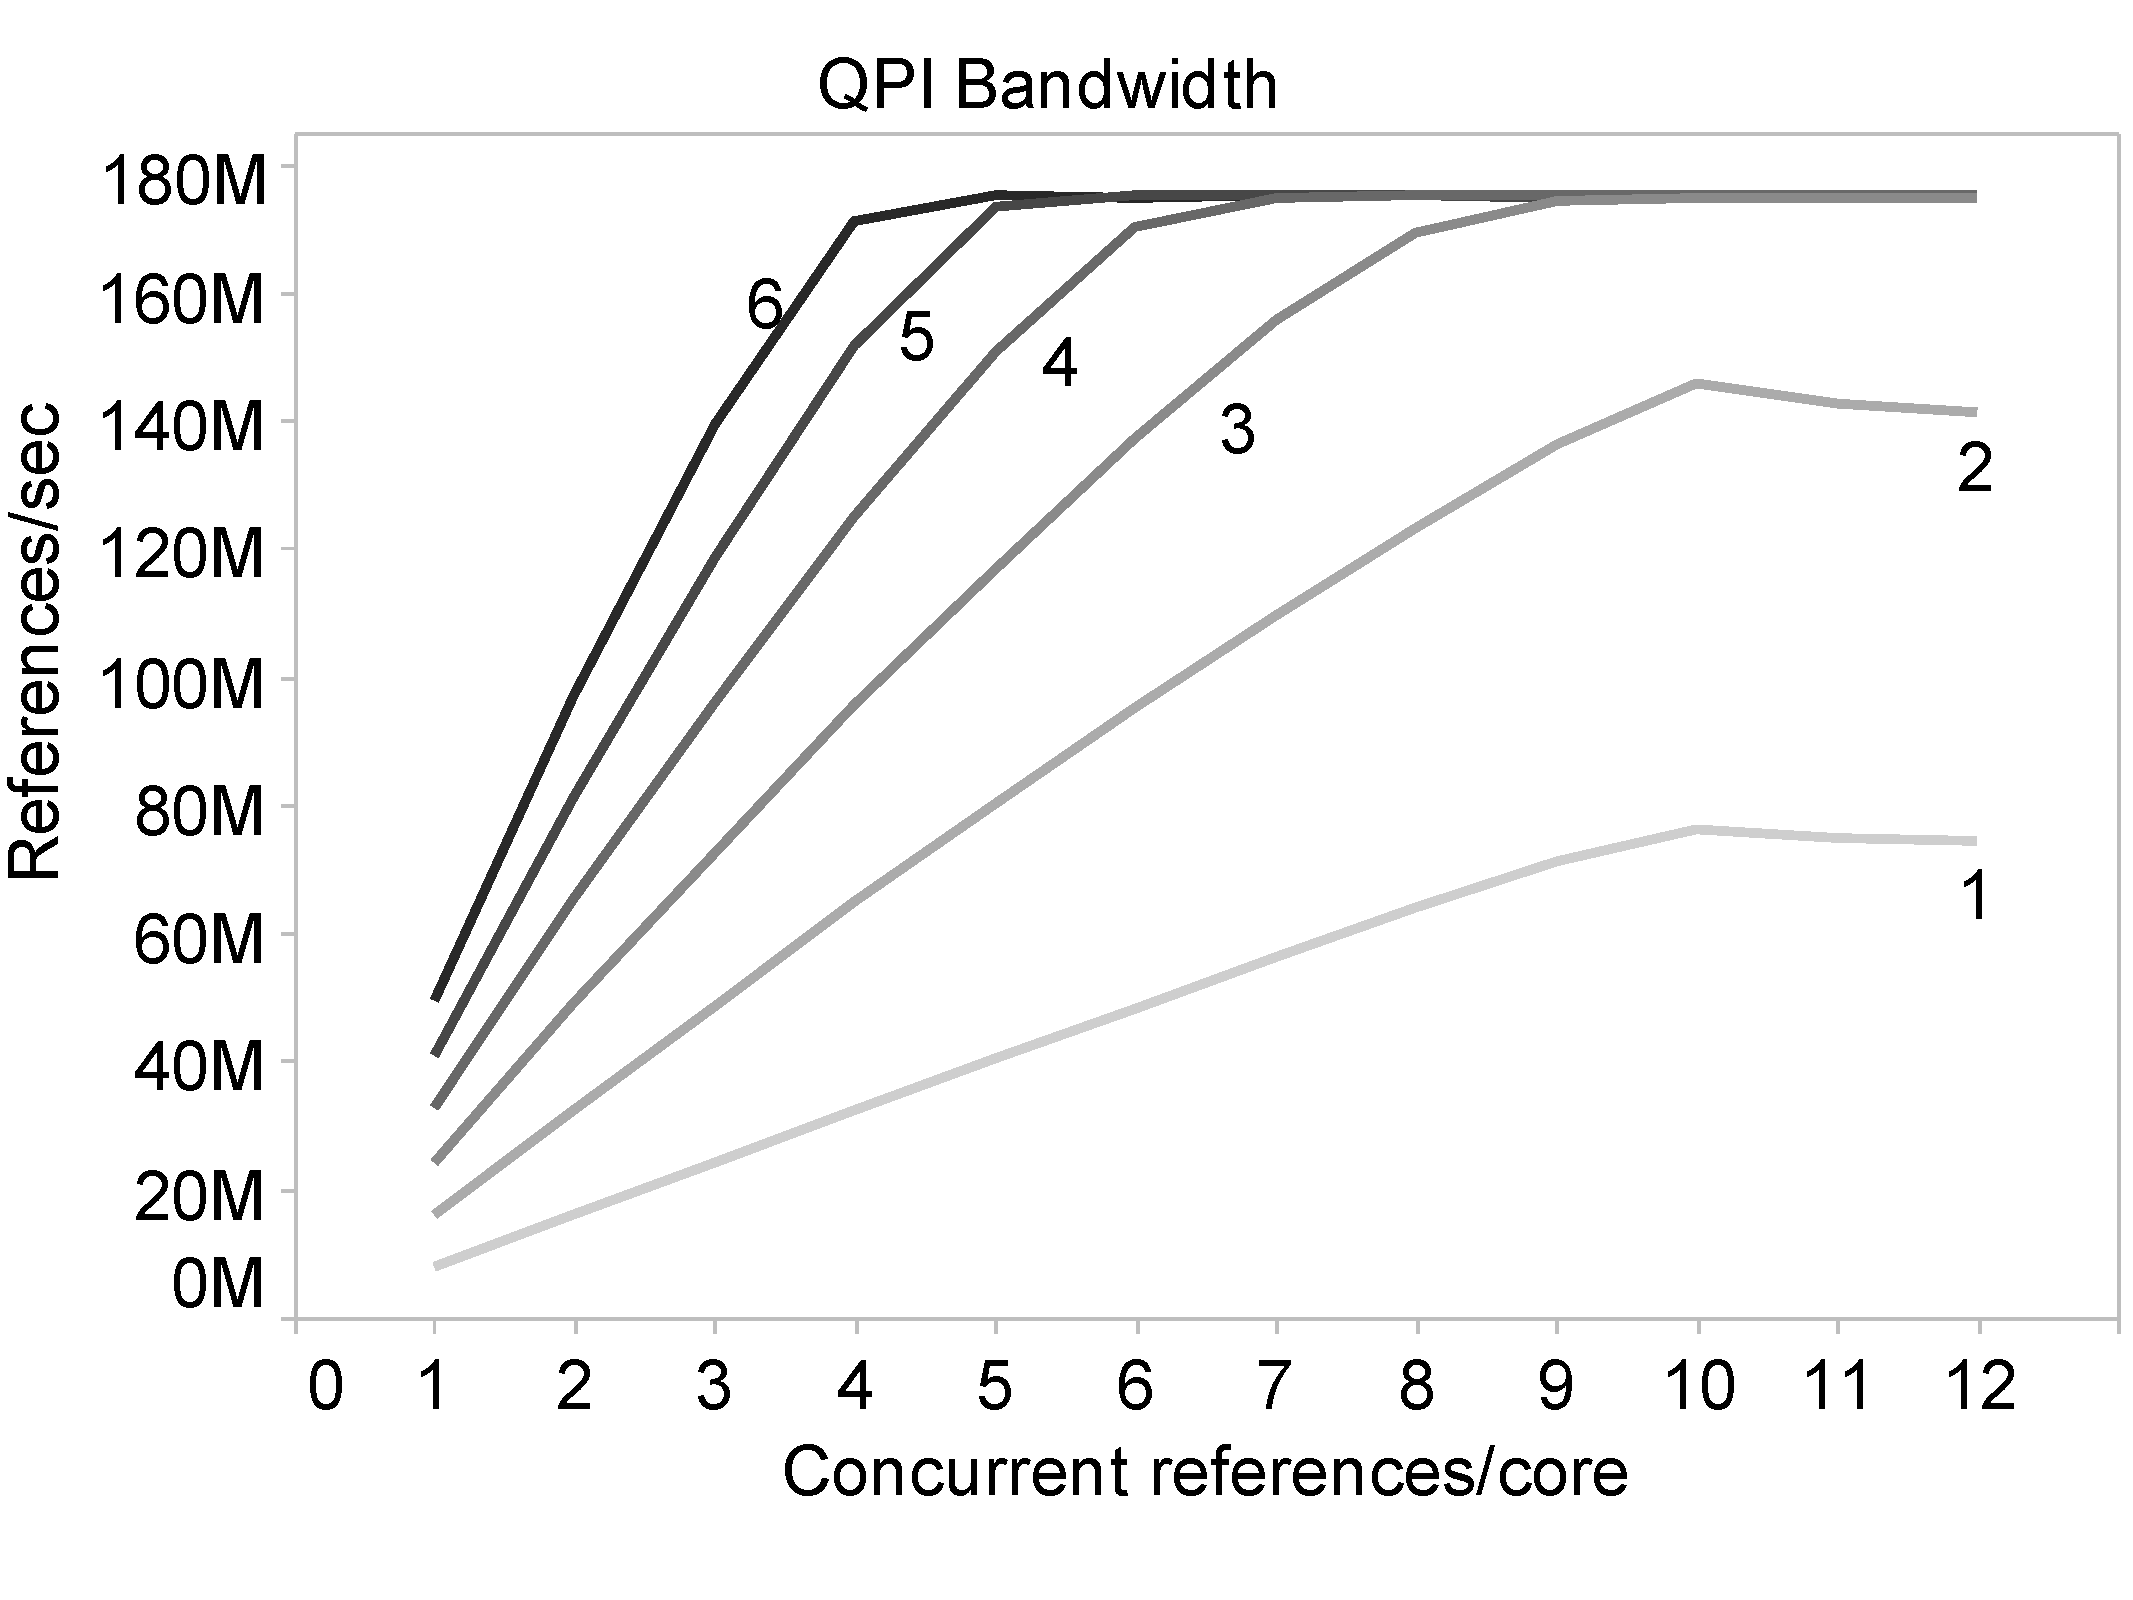
\includegraphics[width=0.5\textwidth]{figures/qpi_bw-edited.pdf}
  \end{center}
  \caption{Pointer chasing in a remote processor's memory.}
  \label{fig:listwalk-qpi}
\end{figure}
%%%%%%%%%%

We measured the rate at which the cores can make requests
over the QPI link. For this experiment, we allocated the lists in the
second chip's memory and ran the traversals on the first chip's cores. Figure~\ref{fig:listwalk-qpi} shows the result. We found that use of the QPI link limits us to 175 million references per second.


To simulate the performance of pointer chasing in a
multi-node system, we modified the scheduler of our coroutine library
to include a delay before a coroutine can be rescheduled, imitating
the network transit delay even though we are referencing local
memory. Recently published measurements of Infiniband latencies
\todo{cite} suggest we might expect 1.1 $\mu$s source-to-destination
latencies between two computers connected back-to-back; we assume a
switch transit delay of 400 ns \todo{how many hops? 1or3?} in each direction and thus estimate a 3
$\mu$s round-trip delay. In this experiment, once a coroutine has
yielded, we use the core's timestamp counter to ensure it does not get
rescheduled for 3 $\mu$s.

\begin{figure}[h]
  \begin{center}
    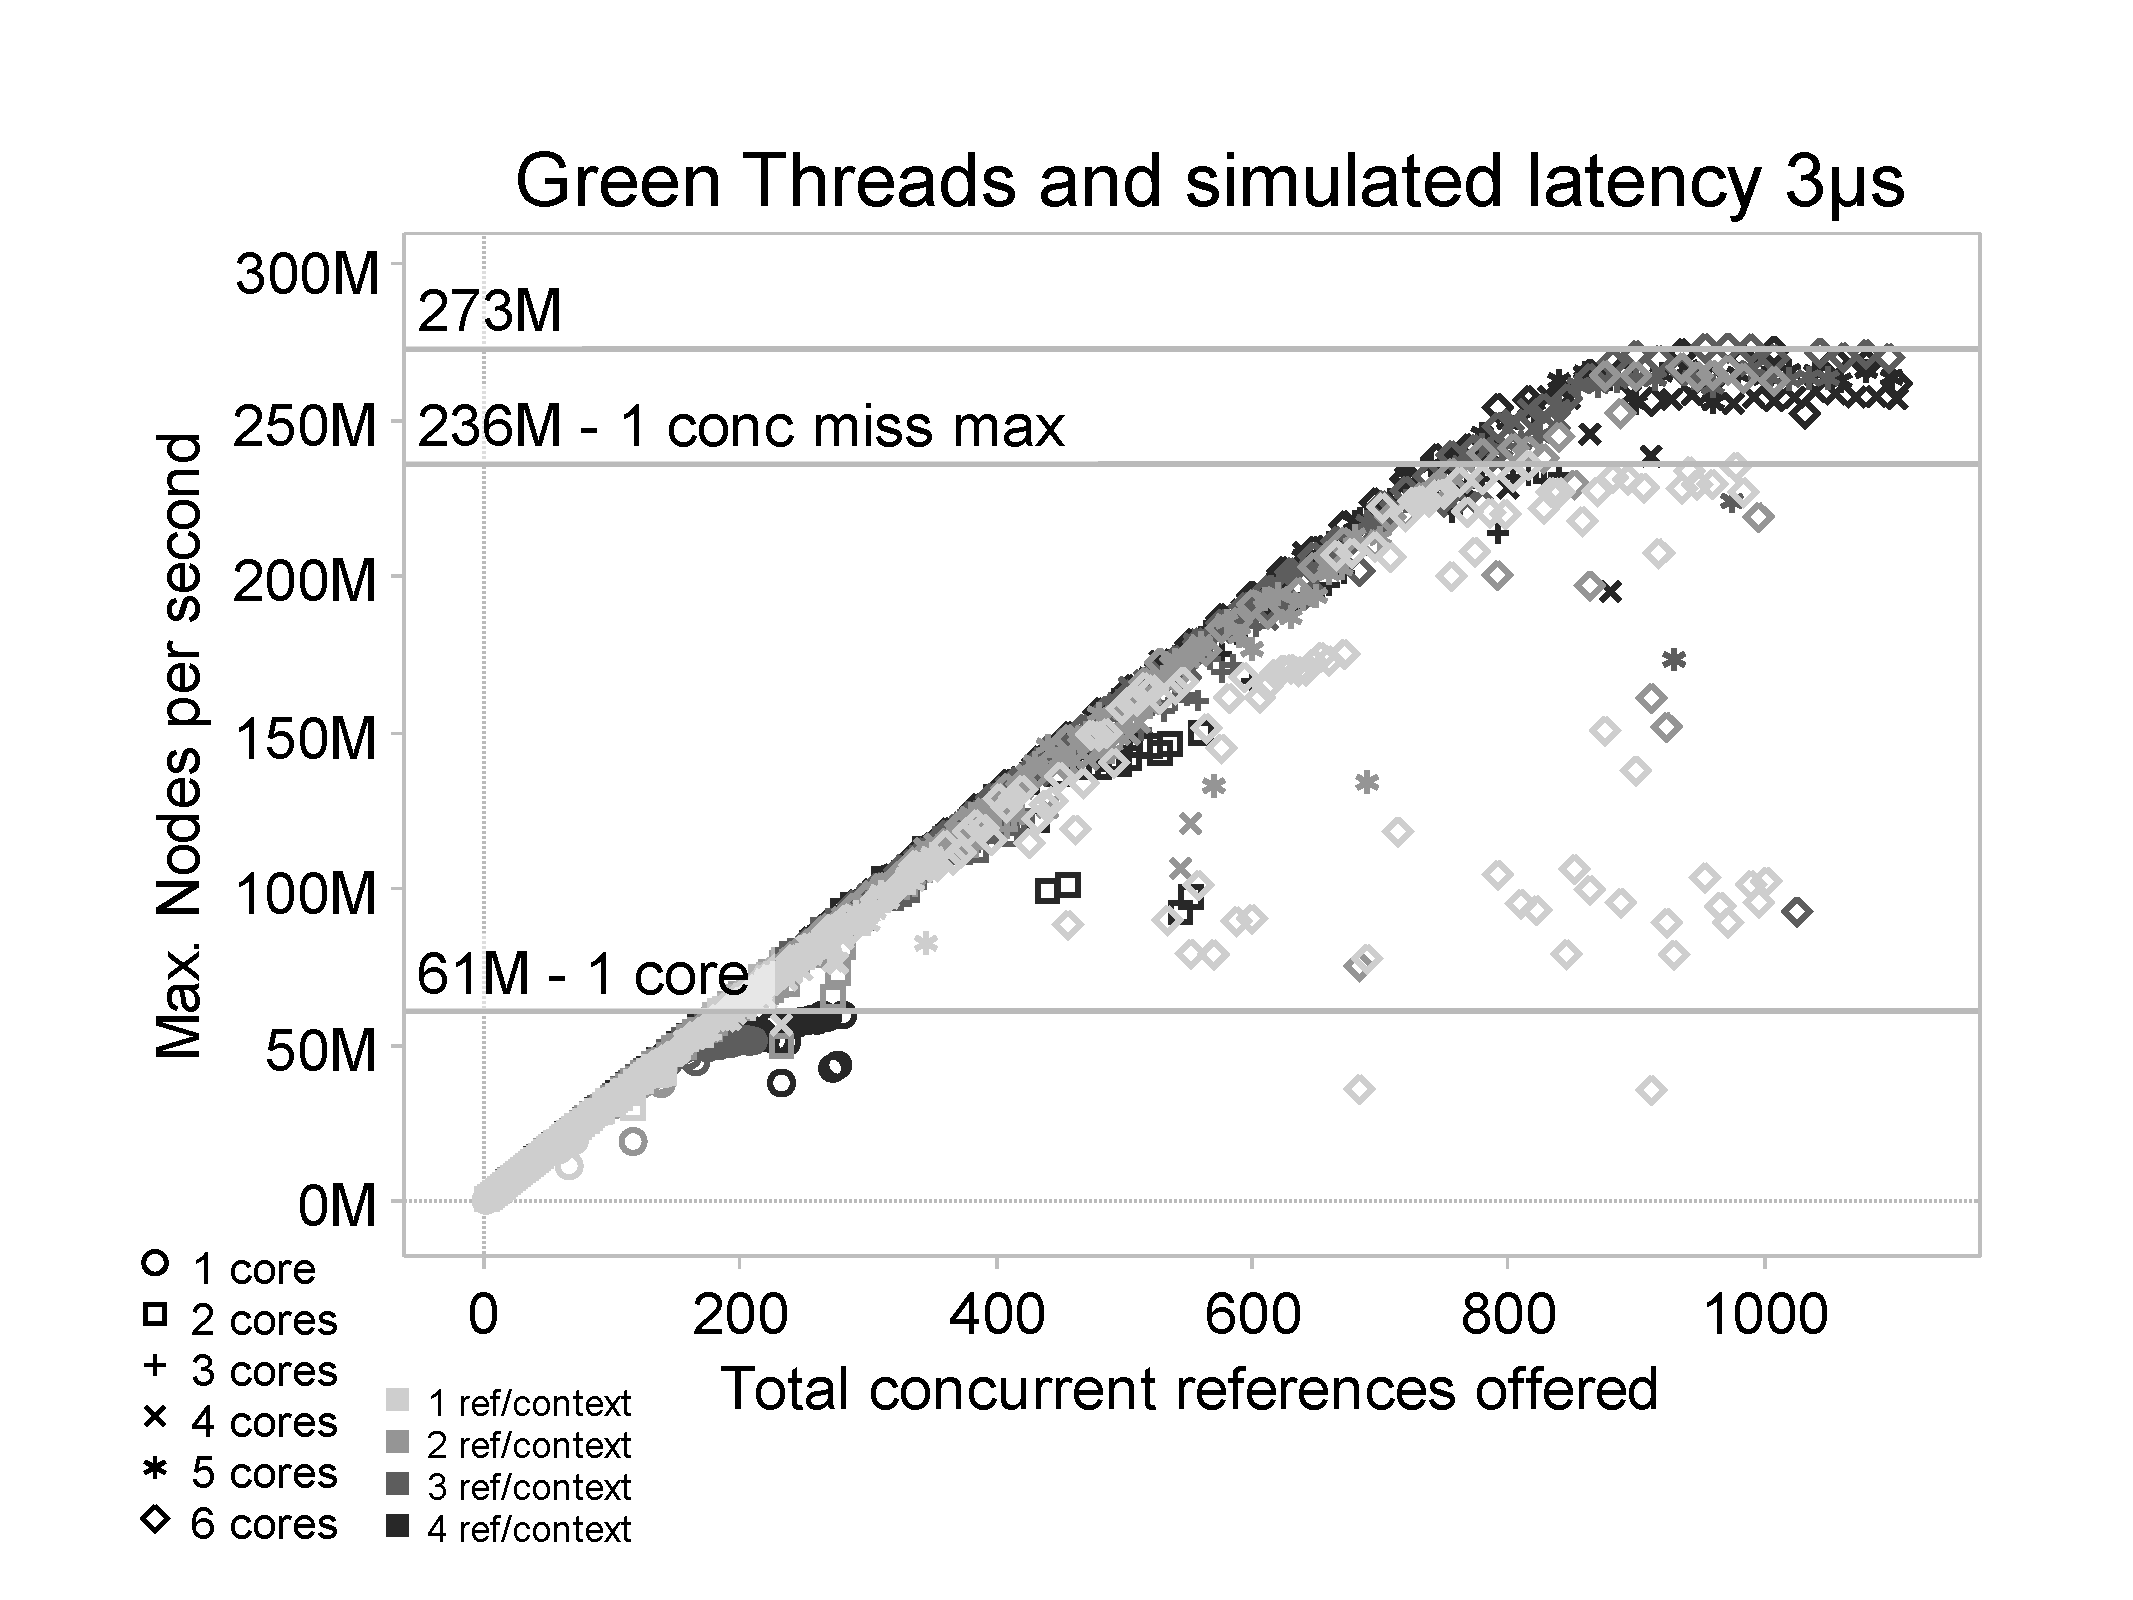
\includegraphics[width=0.5\textwidth]{figures/multi-green-delay7800-edited.pdf}
  \end{center}
  \caption{Pointer chasing with simulated network delay.}
  \label{fig:network-delay}
\end{figure}

We ran these experiments with two sources of memory concurrency: each
core ran up to 167 coroutines, and each coroutine made between 1 and 4
concurrent references. The results are shown in
Figure~\ref{fig:network-delay}. We are still able to reach a
near-maximum rate of 273 million references per second, but at least 2
concurrent references per coroutine are required. Running with a single
reference per coroutine achieves 236 million references per
second. Note that the throughput keeps increasing up to around 850 total concurrent references offered, far more than the 36 we know the chip to support. This is because we have modeled the network latency by forcing coroutines to wait the extra time before using the data, so the physical miss buffers on our machine are not tied up any longer than usual.

We also observe that to achieve a throughput equal to the expected max outgoing network bandwidth (100 million references per second), \todo{reference earlier section calculation?} when there is only one reference per context available, we require 320 coroutines. This is close to the minimum of 300 concurrent references needed to tolerate $3 \mu s$ latency.

Any network interface would be connected through a QPI link,
which we measured to have a bandwidth limit of 175 million references
per second, so our runtime appears to have the capacity to chase pointers
in a remote memory. 

\todo{do we want to include that the memory system imposes max limit so really more throughput is still achievable if there are enough ILP memory concurrency?}\\
\todo{also have results that remote cores over QPI plus delay 3us can make it up to the 175M, with sufficient number of coroutines}


%\todo{Begin eval insert}
%\section{Evaluation}
\label{sec:evaluation}

The goal of our evaluation is to show that the core pieces of the \Grappa
runtime system, namely our tasking system and the global memory/communication
layer work as expected and together are able to efficiently run irregular
applications. We evaluate \Grappa in three basic steps:

\begin{itemize}

\item We present results that show that the \Grappa runtime is able to sustain
very high concurrency rates and the communication layer is able to sustain a
very high rate of global memory operations. We also show the performance of a
graph kernel that stresses communication and concurrency together.

\item We show how some popular irregular applications running on \Grappa
compare to the Cray XMT and hand-tuned MPI code.

\item We finish with a characterization of system behavior, including
profiling where execution time goes, how aggregation affects message size and
rates, how global memory and work stealing behaves.

\end{itemize}

\subsection{Basic \Grappa Mechanisms}
\label{eval:basic}

\paragraph{User-level context switching.}

As discussed earlier, fast context switching is at the heart of \Grappa's
latency tolerance abilities. We assess context switch overheads using a simple
microbenchmark that has a configurable number of workers, where each worker 
just increments values in a large array. 

\begin{figure}[ht]
    \begin{center}
      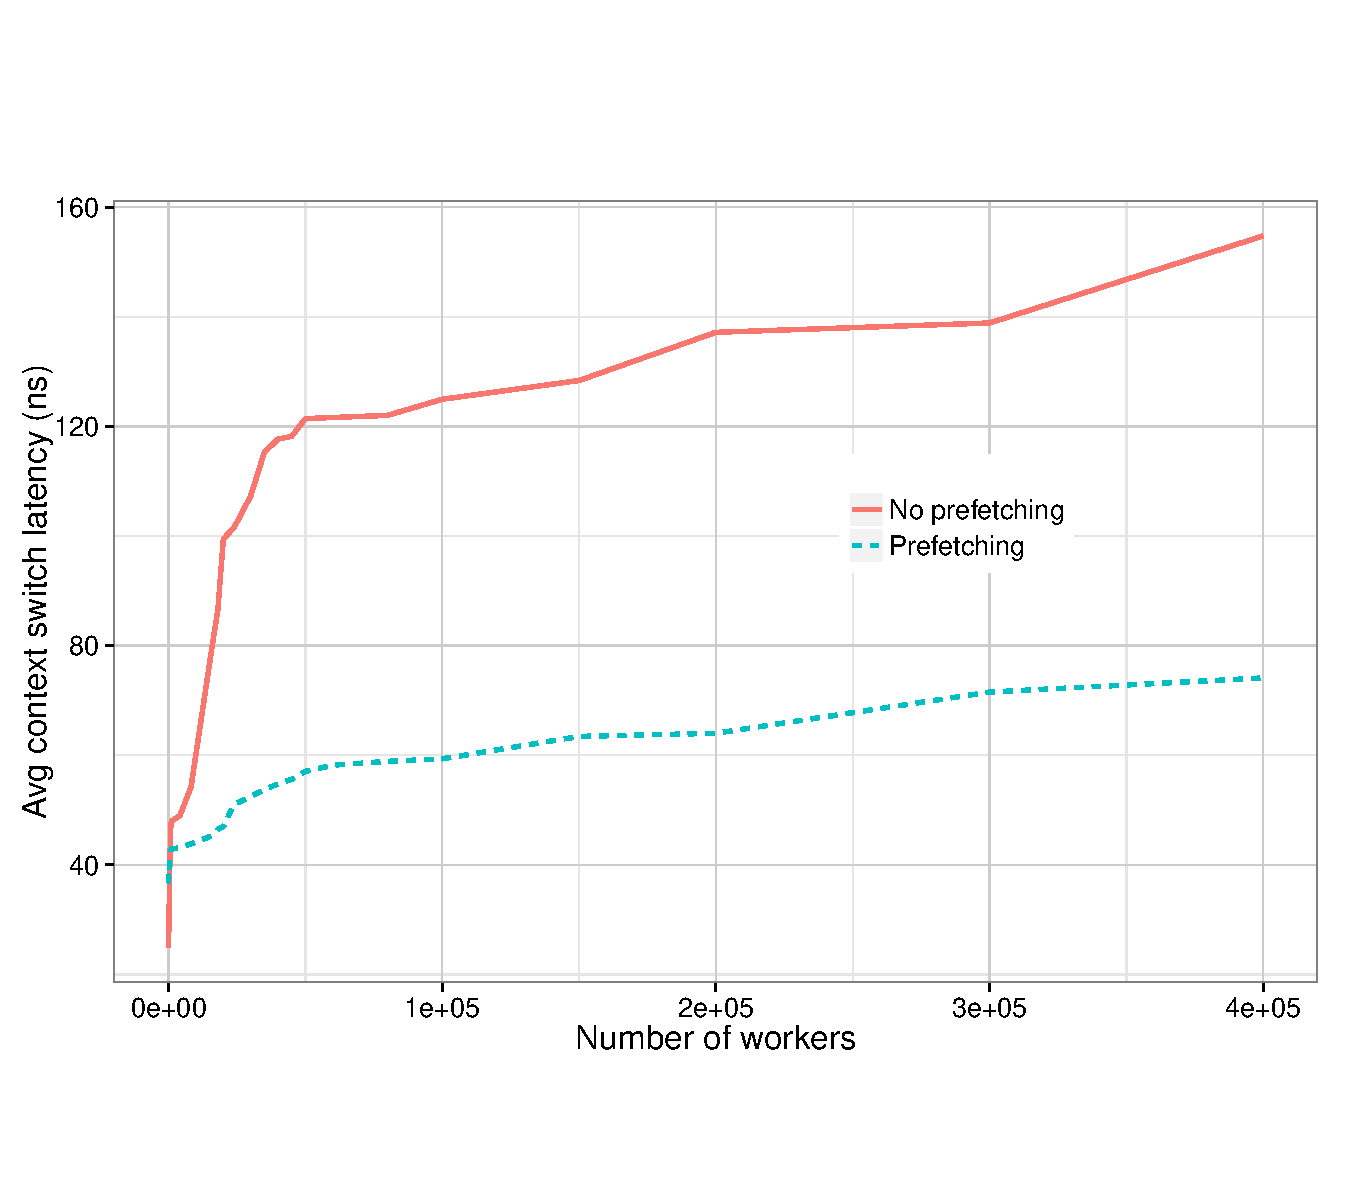
\includegraphics[width=0.5\textwidth]{figs/context_switch_time.pdf}
    \end{center}
    \caption{Average context switch time with and without prefetching.}
    \label{fig:context-switch-exp}
\end{figure}

Figure~\ref{fig:context-switch-exp} shows the average context switch time as
the number of workers grow. There are two important takeaway points from these
data. Context switch time for the number of workers we use ($~$1K workers) is
on the order of 50 ns; and prefetching has significant impact on context
switch time. And context switch time does not grow significantly with the
number of workers --- even with one-half million workers, context switch
is around 75ns.

We also measured (not in the plot) the \emph{rate} of context switch for all
cores in a node, which showed that our rate is limited by off-chip memory
bandwidth. Each context is 4 cache lines (1 for the worker struct and 3 for
stack data), leading to 8 cache line transfers per context switch
(write the previous context, read the next in). The off-chip bandwidth of a
single socket in our system is 270M cache lines per second, which implies that
we can sustain at most 34M context switches per second per socket, which is
almost exactly what we sustain.

In summary, our context switch engine is able to efficiently sustain very high
concurrency and as we will show later, the amount of concurrency sustained is
sufficient the latencies \Grappa needs to hide.

\paragraph{Global memory and communication.} We measure the performance of
\Grappa's global memory and communication layers using a faithful
implementation of the giga updates per second (GUPS) benchmark.
Read-modify-write updates are dispatched at random to a large array. This
benchmark stresses the communication layer of \Grappa separately from the
scheduler, because only a single worker is used per system node.
Figure~\ref{fig:grappa-gups} shows that \Grappa is able to sustain well over a
billion updates per second with 64 nodes. This compares very favorably to
published results~\cite{gups} for other high-end HPC systems.


\begin{figure}[ht]
    \begin{center}
      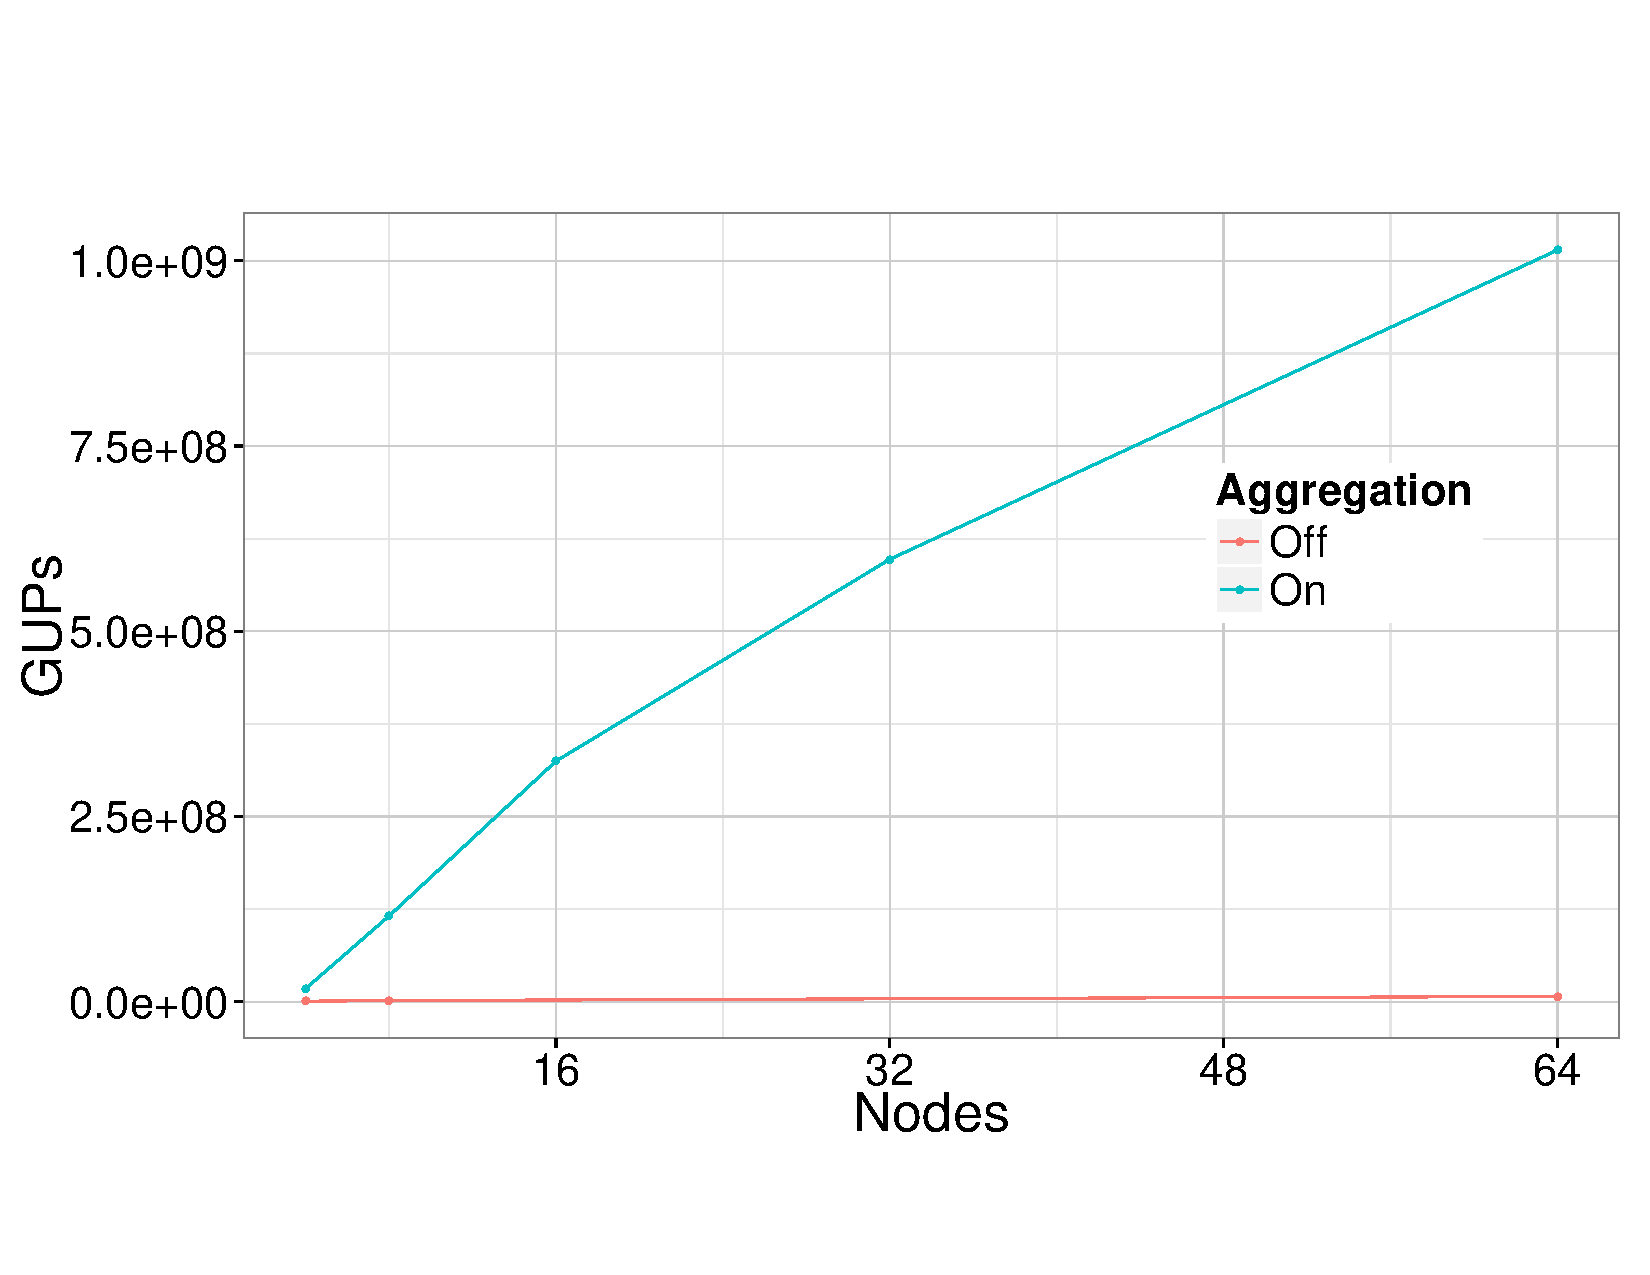
\includegraphics[width=0.5\textwidth]{results/gups/gups.pdf}
    \end{center}
    \caption{GUPS (giga updates per second) for \Grappa as the number of nodes grows.}
    \label{fig:grappa-gups}
\end{figure}

\paragraph{Putting it all together with Unbalanced Tree Search in
    memory (UTS).}
We now show the overall performance of \Grappa running UTS.
Figure~\ref{fig:grappa-uts}. The point of this experiment is to
demonstrate whether \Grappa's context switching and communication layers can in fact
be used together, while balancing workload, to run an irregular application efficiently. 
We look at two classes of trees, T1x and T3x, from the
original benchmark. T1x trees are very shallow and wide, while T3x
trees are very deep. When the access to each vertex is a random
access, the critical path to search T3x trees is very long. On such
trees, we do not expect there to be sufficient concurrency for any
system, including \Grappa, to achieve high throughput. \TODO{plot it
    if time}. To verify this, at the 16-node data point, the average active tasks per
core over the search is 775 and 13 for T1XL and T3L, respectively.

\begin{figure}[ht]
    \begin{center}
      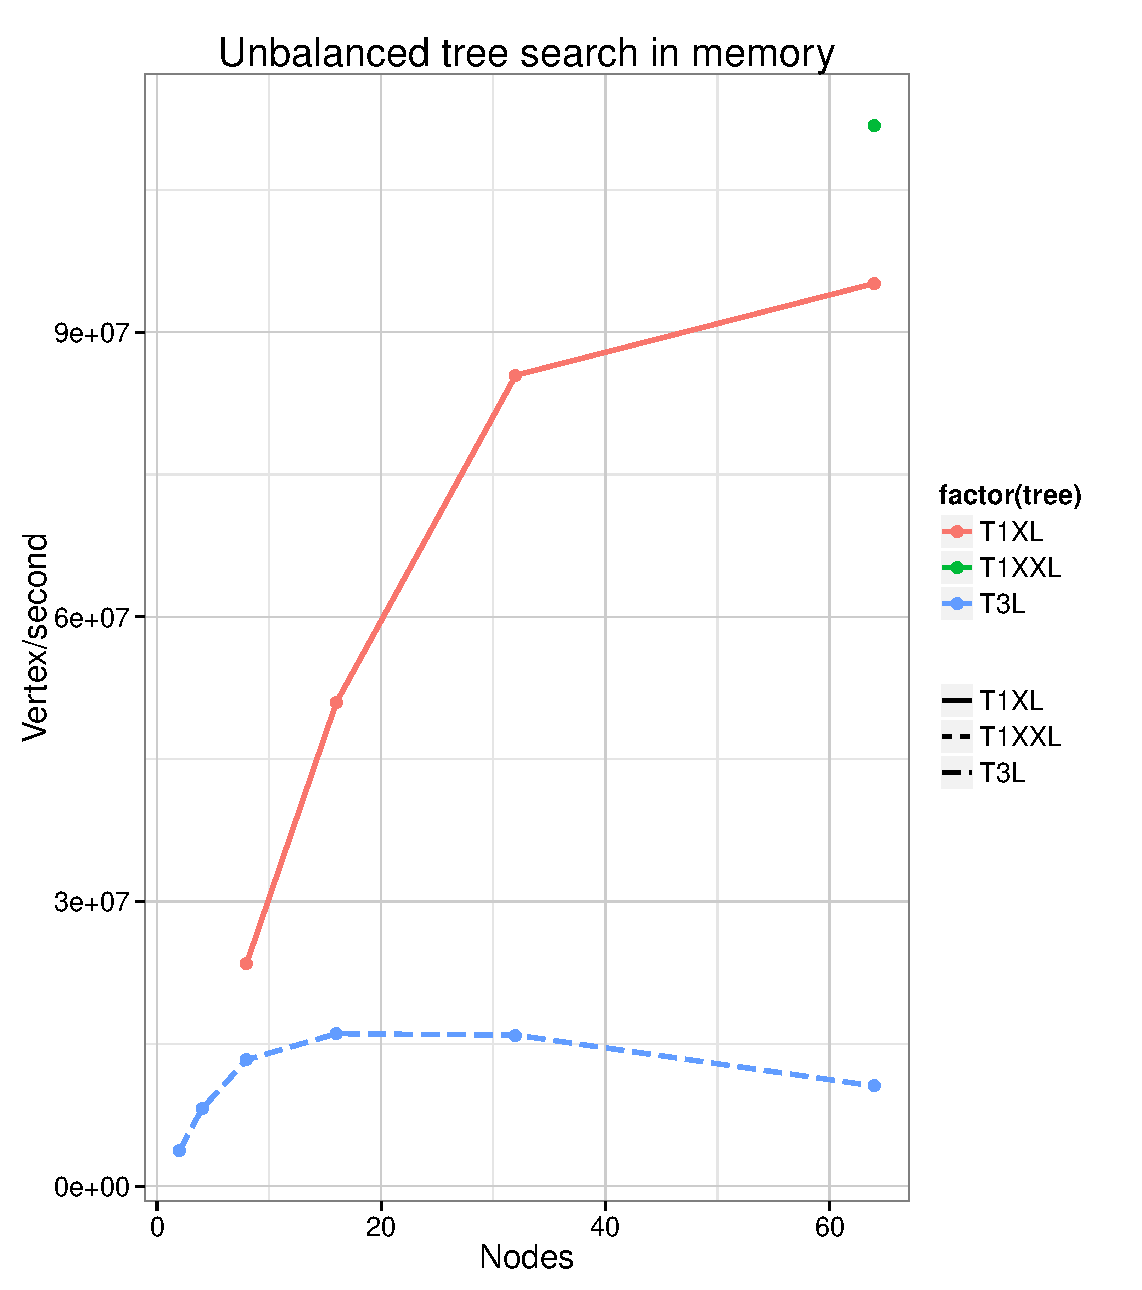
\includegraphics[width=0.5\textwidth]{figs/uts_scale.pdf}
    \end{center}
    \caption{Vertices per second in UTS on \Grappa as the number of nodes grows.}
    \label{fig:grappa-uts}
\end{figure}


\subsection{Comparing \Grappa to Other Systems}

In order to put \Grappa's performance into a general context, we compare it
with XMT running BFS, PageRank, IntSort, GUPS and UTS. Since XMT is a
different hardware platform, we also compare \Grappa with hand-tuned MPI
versions of BFS and GUPS running on the same hardware. Finally, we also
compare it with UTS written for UPC. We run all experiments with 64 nodes.

\begin{figure}[ht]
    \begin{center}
      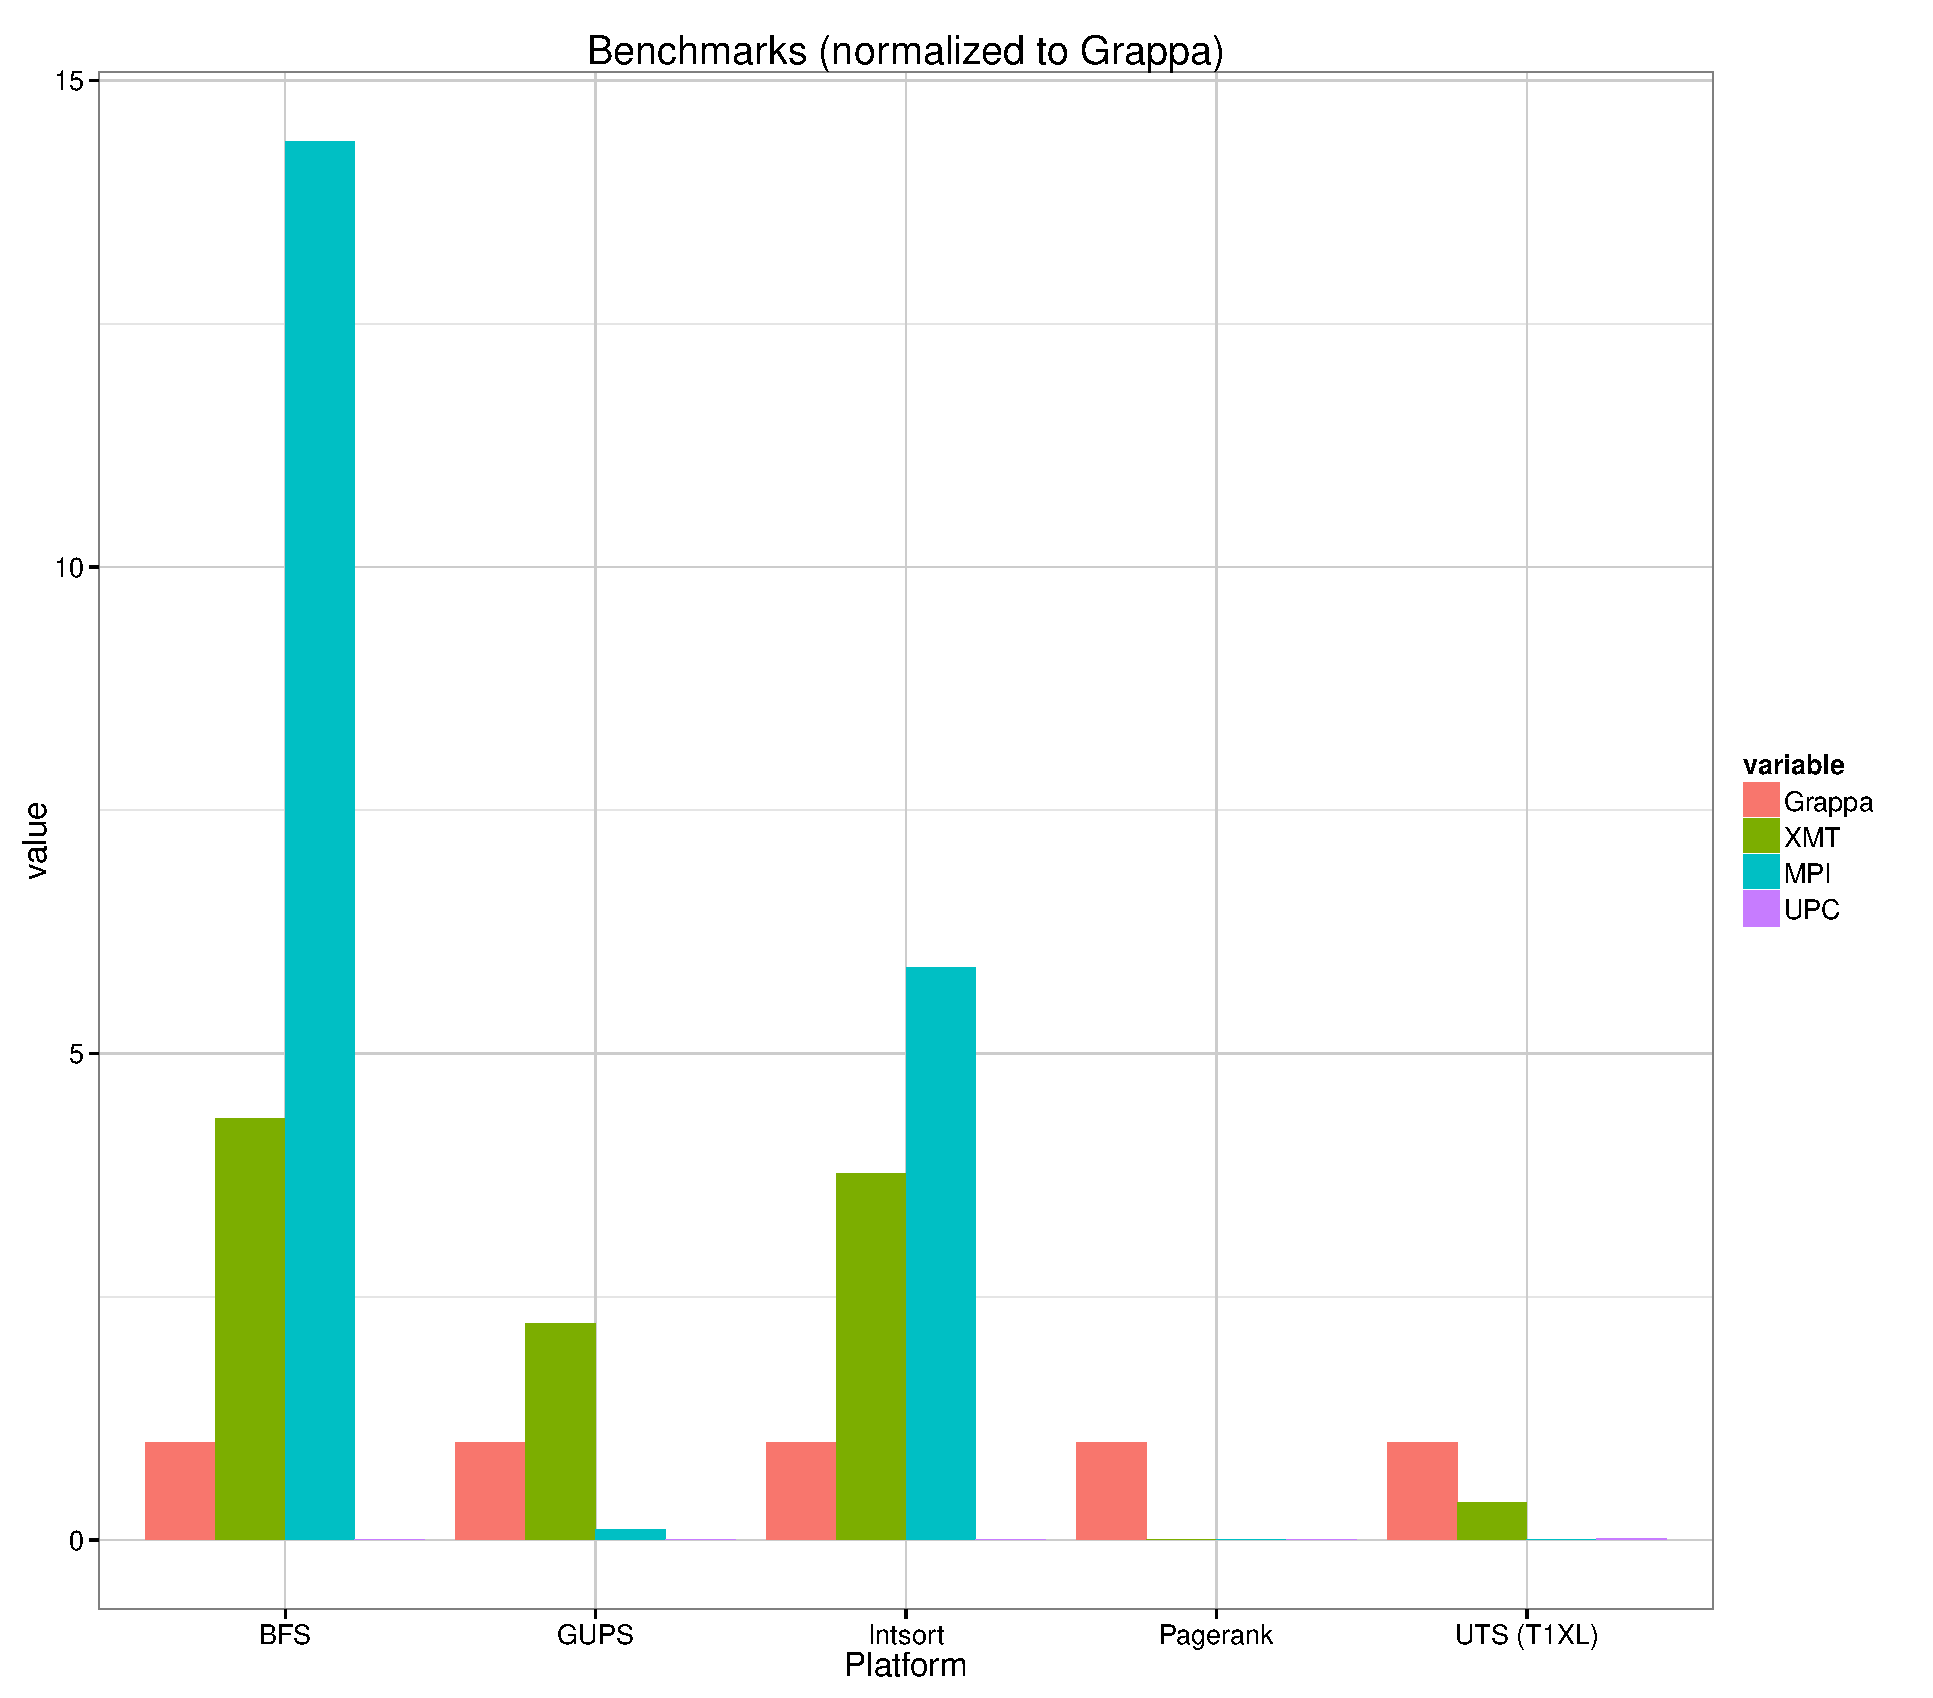
\includegraphics[width=0.5\textwidth]{results/benchmarks.pdf}
    \end{center}
    \caption{Comparing \Grappa with XMT, hand-tuned MPI and UPC.}
%bar chart, one set of bars per benchmark, one bar per system. runtime normalized to grappa.
    \label{fig:grappa-comparisons}
\end{figure}

Figure~\ref{fig:grappa-comparisons} shows the results. Overall, \Grappa is
within striking distance of XMT and UPC performance. However, it underperforms
compared to hand-tuned MPI. Nevertheless, this comparison needs to be taken
with a grain of salt for several reasons. First, we have not spent as much
time tuning \Grappa's implementations. This is supported by inspecting the BFS
MPI implementation we used, which clearly shows that it employs a lot of
algorithmic-specific optimizations. In fact, some of these optimizations
resemble some of what \Grappa does automatically, like message aggregation.
Second, the GUPS results presented earlier suggests that \Grappa performance
can do a lot better. \TODO{update this once we have more results. }

\subsection{Characterization}

\paragraph{Where execution time goes.}


\begin{figure}[ht]
    \begin{center}
      \begin{tabular}{c|c c c c}
        Benchmark     & Comm & User & Idle & Sched \\ \hline
        GUPS          & 6.60  & 42.94   & 47.74 & 2.80 \\
        BFS           & 54.84 & 30.90   & 10.94 & 3.43 \\ 
        Intsort       & 34.28 & 42.00   & 21.31 & 2.47 \\ 
        UTS           & 40.57 & 56.52   &  1.21 & 1.73 \\
        Pagerank      & 76.79 & 20.71   &  0.06 & 2.50 \\
      \end{tabular}
    \end{center}
    \caption{\Grappa\ execution time profile, in percent.}
%bar chart, one set of bars per benchmark, one bar per system. runtime normalized to grappa.
    \label{fig:grappa-profile}
\end{figure}

\TODO{PAGERANK:
    Without parallelizing the dot product, \Grappa cannot achieve
high utilization of workers proportional to the size of the data set.
Also mention that the cost of this is contention at the target
elements of vector.  The other parts of pagerank are super fast
(table?)
}

\paragraph{Message size and latency.}
Distribution if possible. With and without aggregation. 

\begin{figure}[ht]
    \begin{center}
      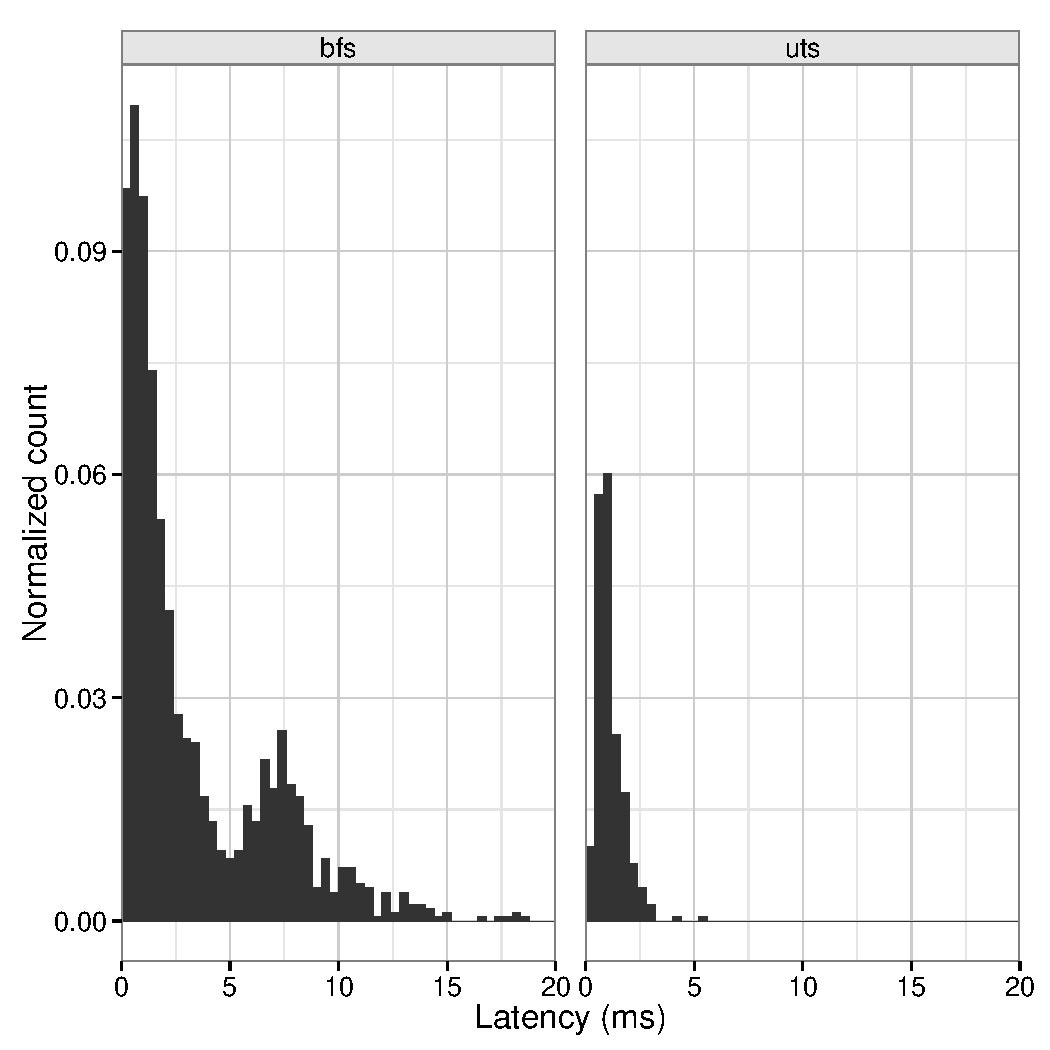
\includegraphics[width=0.5\textwidth]{results/histograms/latency_cmb.pdf}
    \end{center}
    \caption{Round-trip latency of delegate operations.}
%bar chart, one set of bars per benchmark, one bar per system. runtime normalized to grappa.
    \label{fig:grappa-latency}
\end{figure}

\begin{figure}[ht]
    \begin{center}
      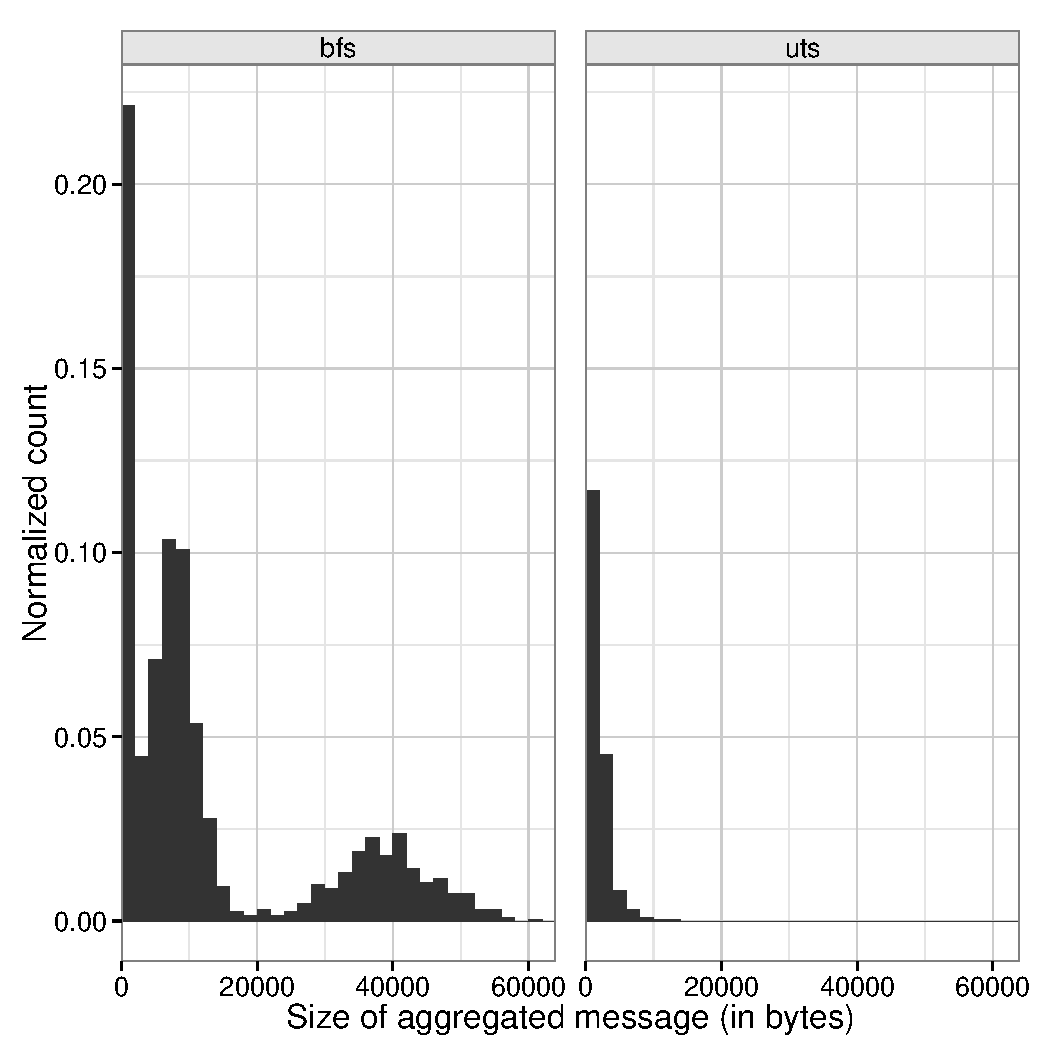
\includegraphics[width=0.5\textwidth]{results/histograms/rdma_bytes_sent_histogram_cmb.pdf}
    \end{center}
    \caption{Distribution of aggregated message sizes.}
%bar chart, one set of bars per benchmark, one bar per system. runtime normalized to grappa.
    \label{fig:grappa-message-size}
\end{figure}


\paragraph{Frequency of remote requests.}

\paragraph{Work stealing behavior.}
Performance loss of not having stealing. Ratio of \# of steals over total \# of task spawns. UTS needs stealing to work. 
















%%%%%%%%%%%%%%%%%%%%%%%%%%%%%%%%%%%%%% OLD %%%%%%%%%%%%%%%%%%

\comment{


Our evaluation begins with presentation of microbenchmark results, establishing
the intrinsic potential of \Grappa to provide random access bandwidth and latency tolerance. 
Next, we present application results, both for \Grappa and for other paradigms, as well
as comparing against the Cray XMT.  Finally, we present the impact of increased aggregation delay
on \Grappa results, thus exploring robustness to network scale.

\subsection{Microbenchmark Results}

\subsubsection{Random Access}
\TODO{Random access feed forward results on \Grappa.  optional: Results we measured for XMT.  Cite MPI results}
\subsubsection{Latency Tolerance}
\TODO{Simple ping test results -- eg, MPI ping, not the full blown aggregation ping test.  Random access blocking results on \Grappa.}
\subsubsection{Scheduling and Robustness}

\begin{figure}[ht]
    \begin{center}
      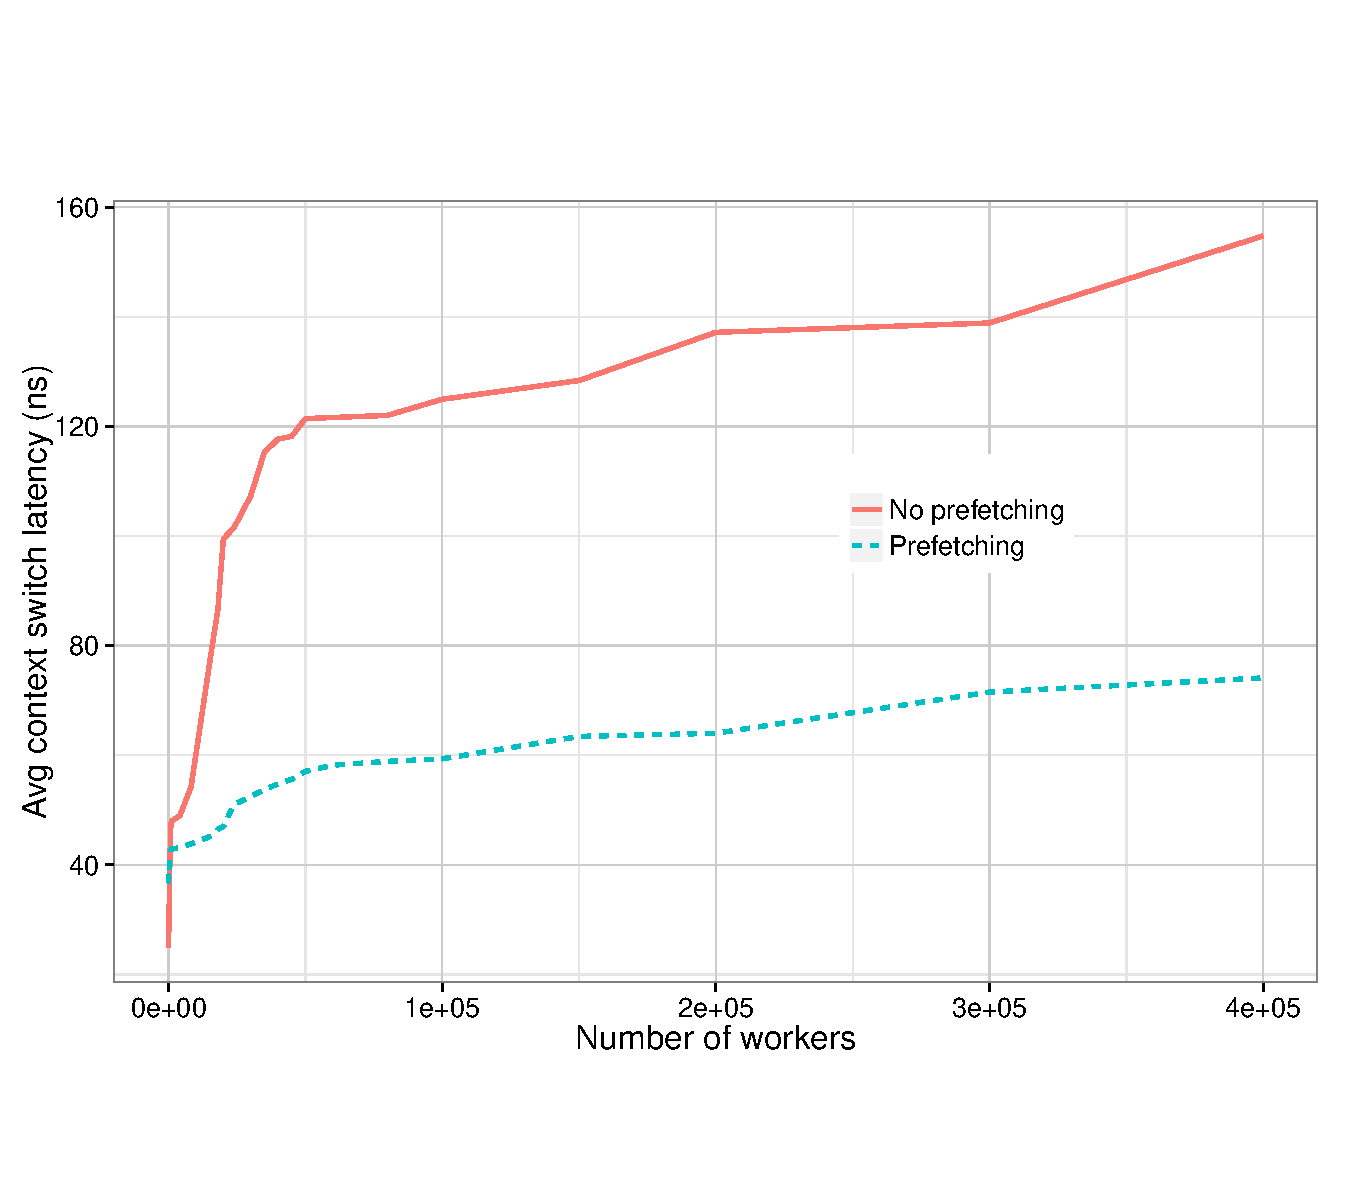
\includegraphics[width=0.5\textwidth]{figs/context_switch_time.pdf}
    \end{center}
    \caption{Average context switch time with 1 and 6 active cores,
        with and without prefetching.}
    \label{fig:context-switch-time}
\end{figure}

\begin{figure}[ht]
    \begin{center}
      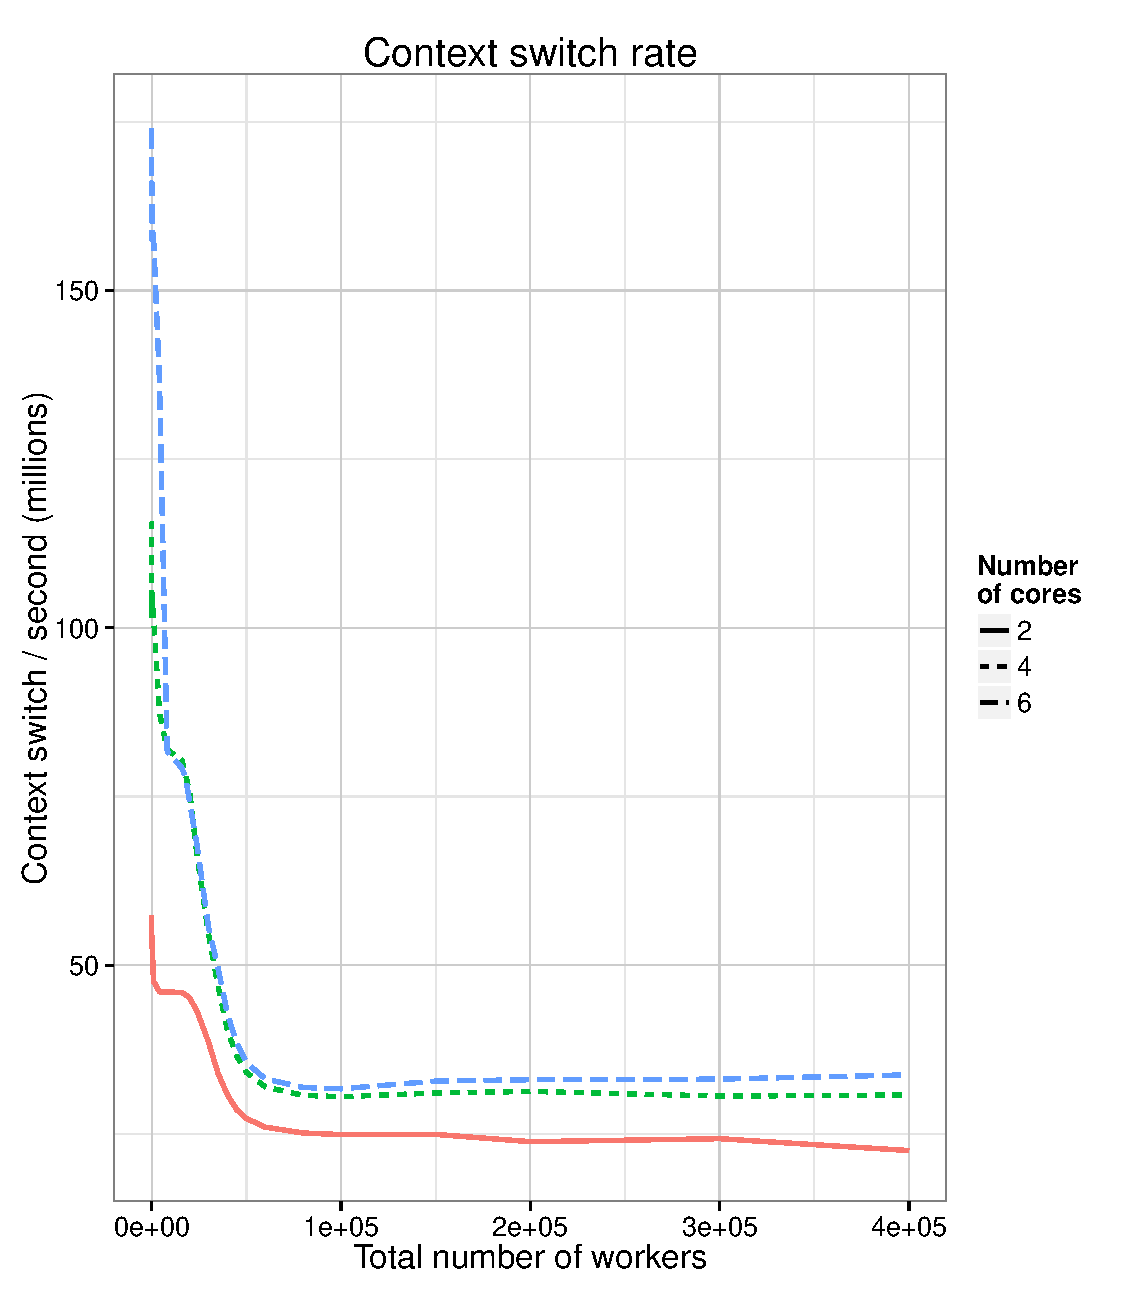
\includegraphics[width=0.5\textwidth]{figs/context_switch_bw.pdf}
    \end{center}
    \caption{Context switch rate with prefetching. Once the total
        size of contexts sufficiently exceeds last-level cache, most
    prefetches go to main memory and the rate becomes limited to the
    off-chip bandwidth.}
    \label{fig:context-switch-time}
\end{figure}

\TODO{Summary of what to write please expand: Reference above plots. Bandwidth of single socket is
    270Mcacheline/s. Each context is 4 cachelines: 1 for worker struct
    and 3 stack cachelines. We must read and write every context, so 8
    cacheline transfers per context switch. This asymptotically
    approaches 33.75Mcontexts/s as you increase the number of contexts
    (fewer and fewer in L3). Note that only 4+ cores reaches full rate
    because these westmere chips are balanced to not achieve full off-chip bandwidth until 4
    cores--bdmyers}

\TODO{Yield test results:  latency \& bandwidth.  Discussion of implications of zillions of contexts on robustness of latency tolerance preshadowing ~\ref{sec:scaling}}

\subsection{Application Results}
To evaluate \Grappa's performance with respect to the XMT, we ran each
of our three benchmarks on up to 16 nodes of each machine. \Grappa used
6 cores per node, with the best parameters chosen for each point. In
some cases, the XMT could not run the benchmark with 2 nodes, so the
point is omitted. \TODO{rewrite this!}
\subsubsection{Unbalanced Tree Search}\TODO{rewrite with new results}
%% UTS: performance comparison
\begin{figure}[ht]
    \begin{center}
      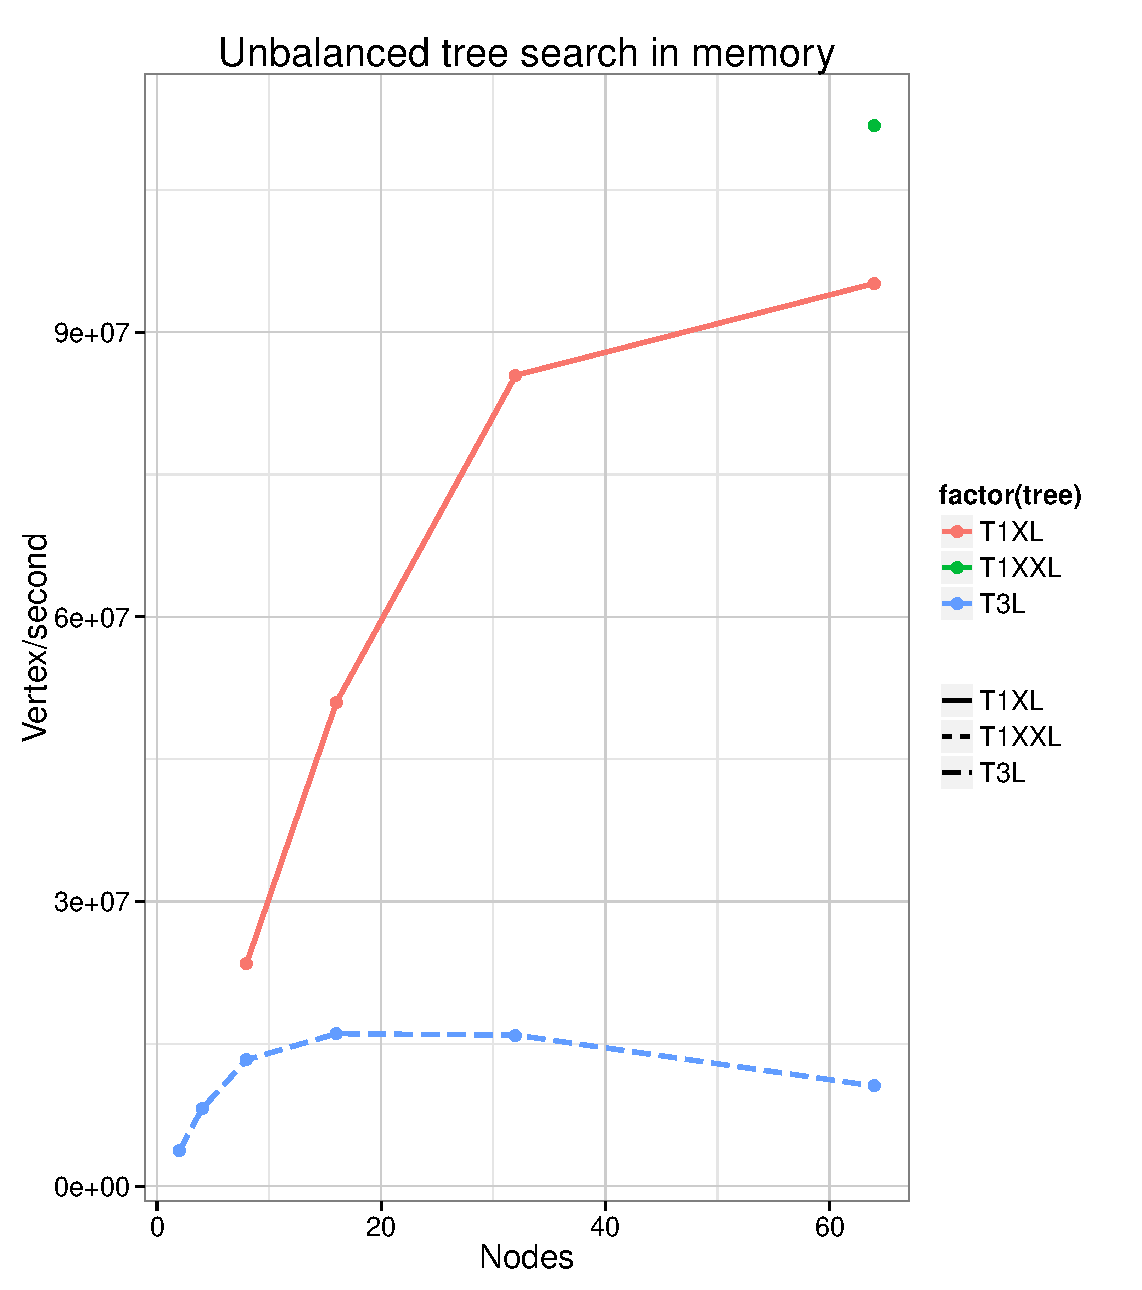
\includegraphics[width=0.5\textwidth]{figs/uts_scale.pdf}
    \end{center}
    \caption{Performance of in-memory unbalanced tree search.}
    \label{fig:uts_compare}
\end{figure}

We ran UTS-mem with a geometric 100M-vertex tree
(T1L). Figure~\ref{fig:uts_compare} shows the performance in terms of
number of vertices visited per second versus number of compute
nodes. \Grappa is 3.2 times faster than the XMT at 16 nodes.  As we will show later, the performance advantage \Grappa has over XMT increases as more nodes are added.  The main reason \Grappa performs better is the software-based delegate synchronization obviates the need for the retry-based synchronization that XMT uses.

\subsubsection{Breadth First Search}\TODO{rewrite with new results}
\begin{figure}[tH]
\begin{center}
  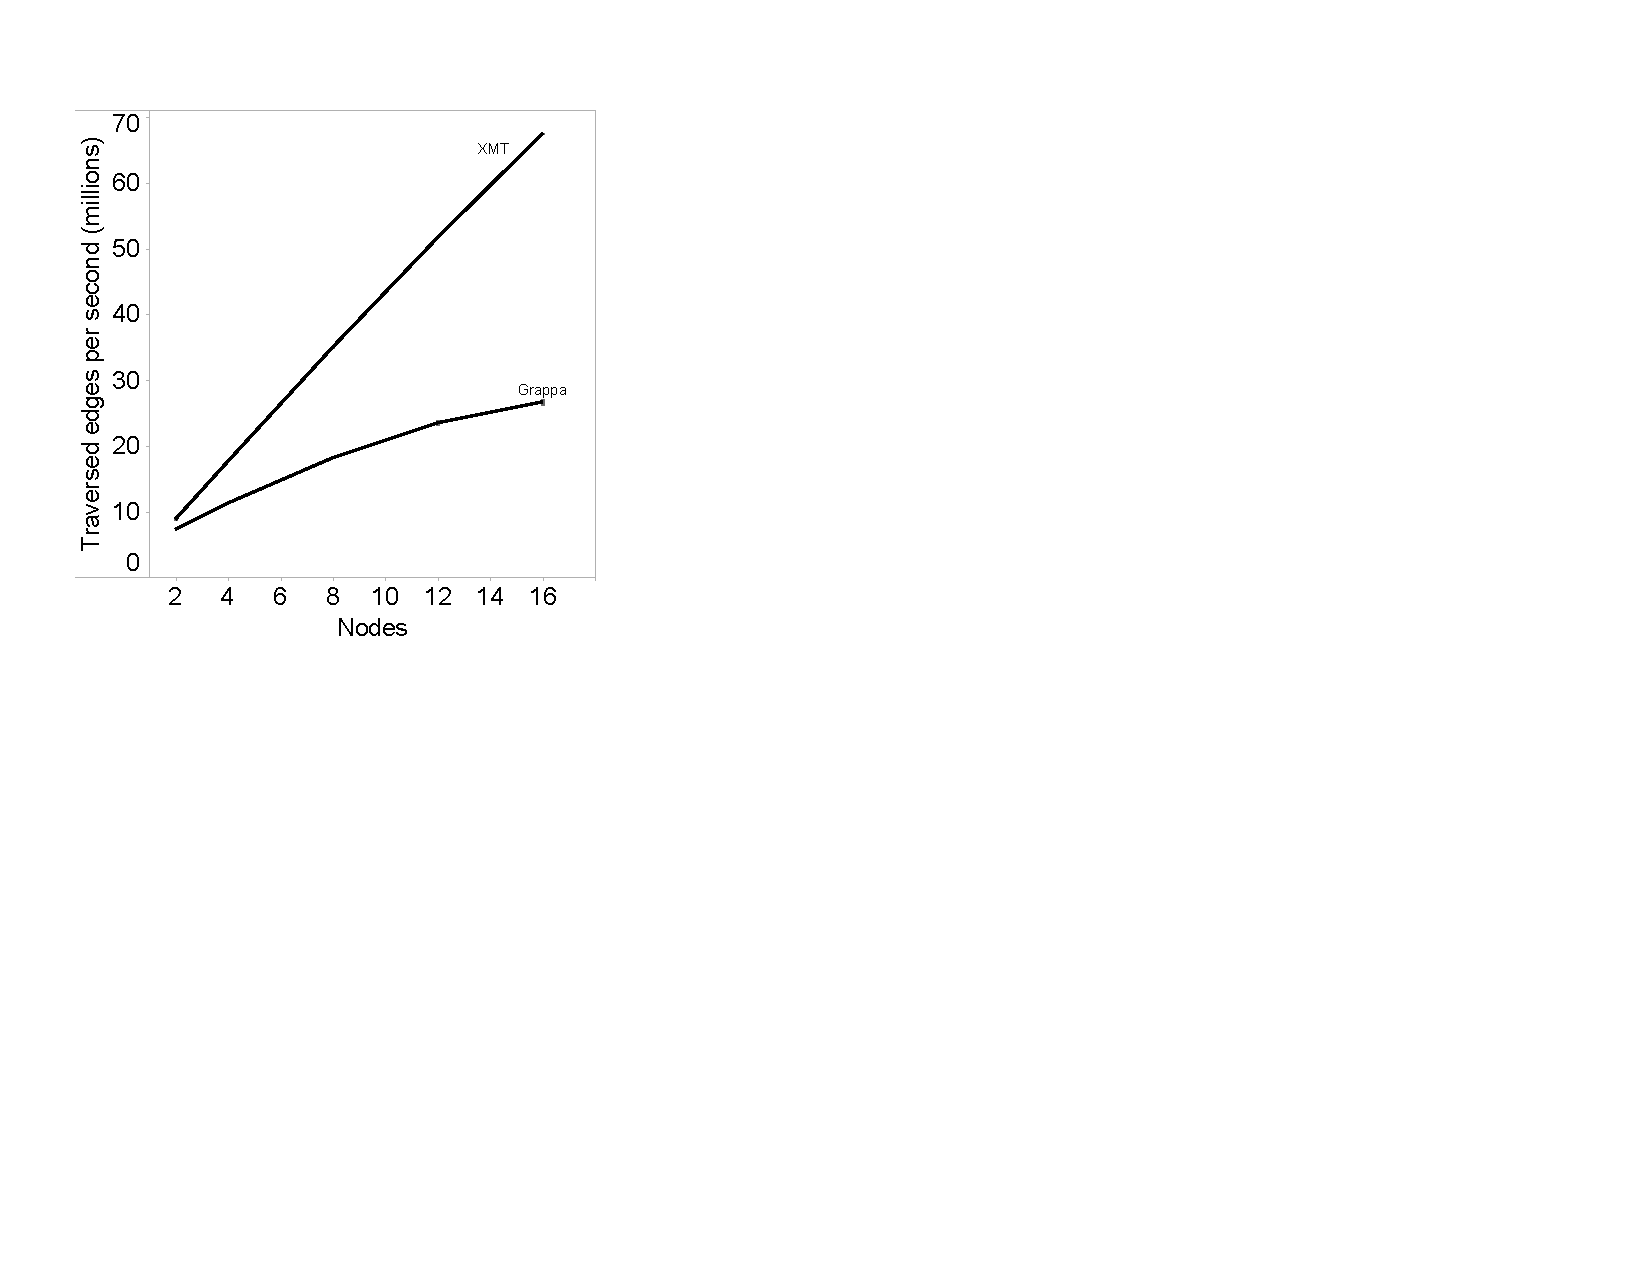
\includegraphics[width=0.95\columnwidth]{figs/bfs_performance}
\begin{minipage}{0.95\columnwidth}
  \caption{\label{fig:bfs-performance} BFS performance}
\end{minipage}
\vspace{-3ex}
\end{center}
\end{figure}

We ran BFS on a synthetic Kronecker graph with $2^{25}$ vertices and
$2^{29}$ edges (25 GB of data). Figure~\ref{fig:bfs-performance} shows
our performance in terms of graph edges traversed per second. The XMT
is 2.5 times faster than \Grappa at 16 nodes.  Performance does scale at a constant rate for \Grappa, suggesting that adding more nodes will increase performance.

\subsubsection{Approximate Betweenness Centrality}\TODO{rewrite with new results}
\begin{figure}[tH]
\begin{center}
  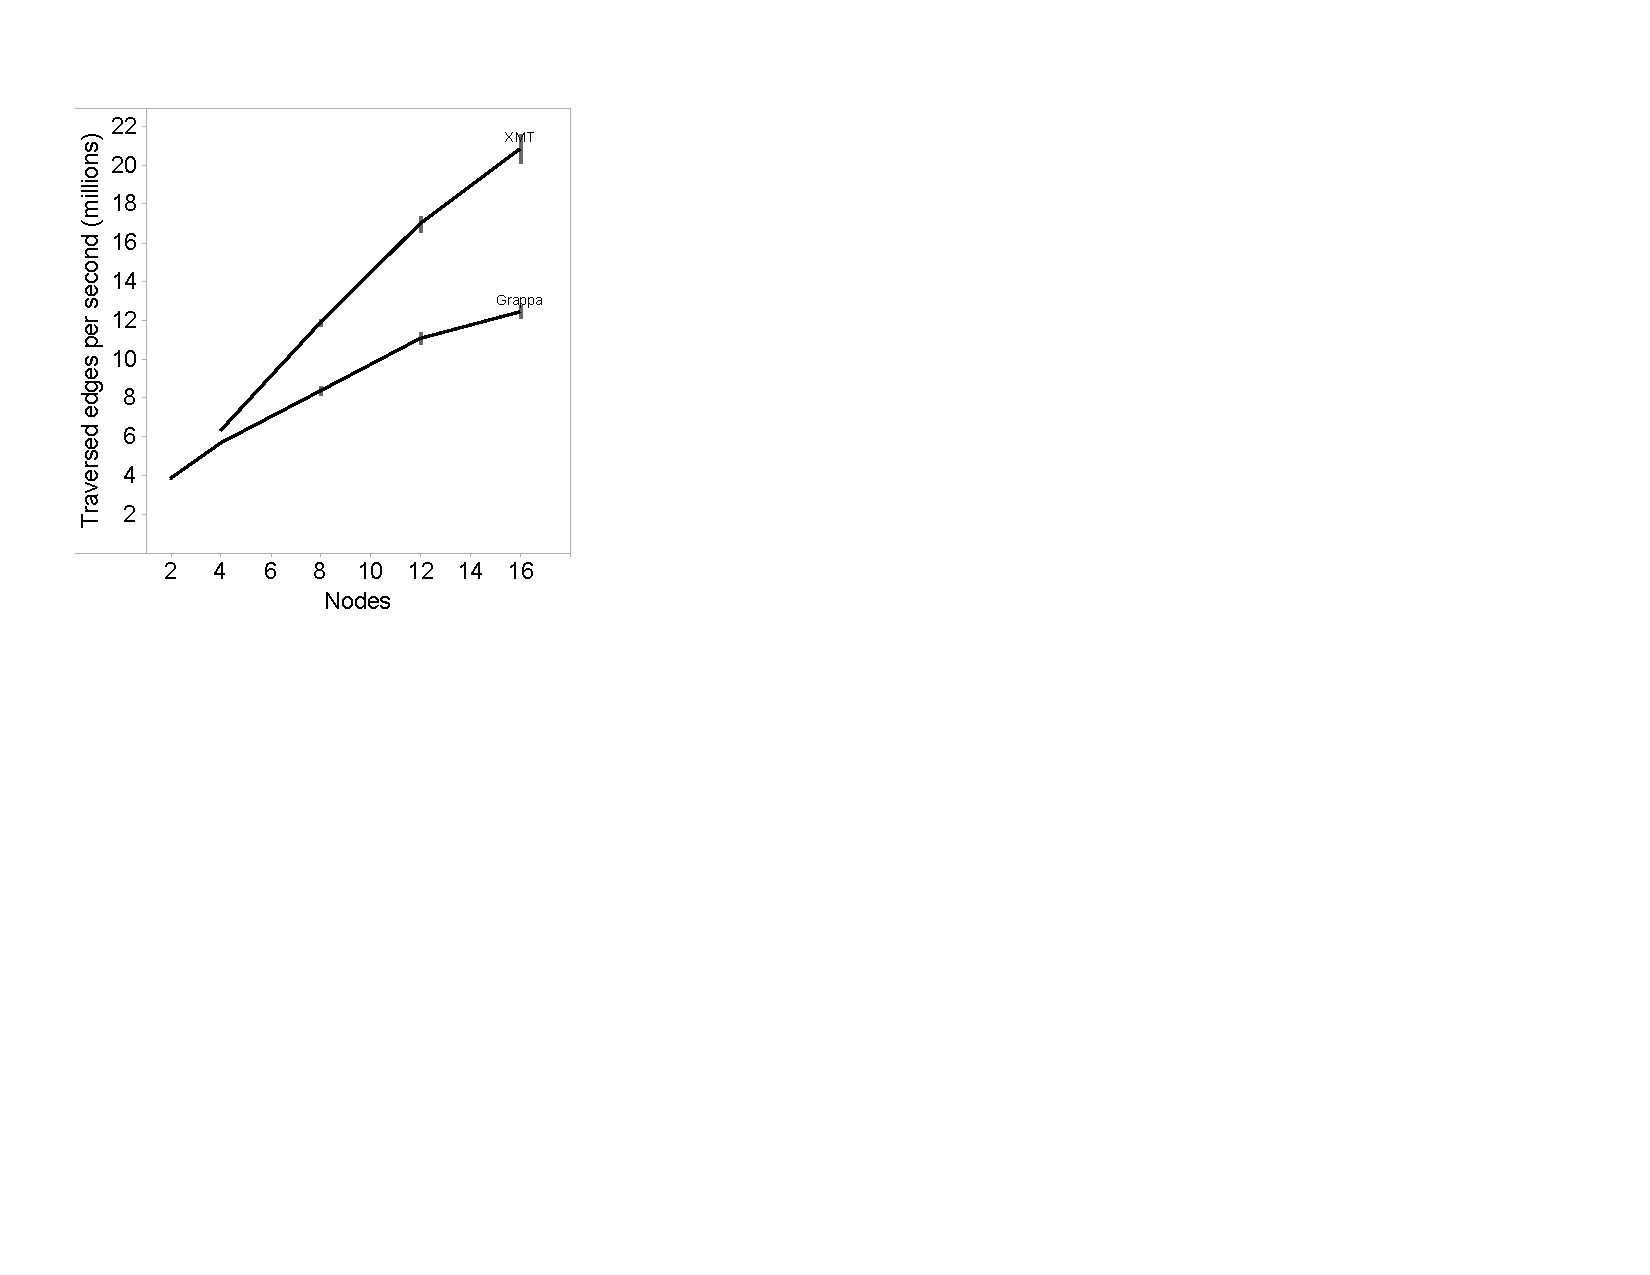
\includegraphics[width=0.95\columnwidth]{figs/centrality_performance}
\begin{minipage}{0.95\columnwidth}
  \caption{\label{fig:centrality-performance} Centrality performance}
\end{minipage}
\vspace{-3ex}
\end{center}
\end{figure}

We ran Betweenness Centrality on the same scale 25 Kronecker graph as
we did for BFS. Figure~\ref{fig:centrality-performance} shows our
performance in terms of graph edges traversed per second. At 16 XMT
processors/cluster nodes, the XMT is 1.75 times faster than \Grappa.

% Got rid of this discussion of UTS by itself, tried to work the highlights in below
%\paragraph{UTS-Mem}
%We ran UTS-Mem on \Grappa and the XMT with a geometric 1.6B-vertex tree
%(T1XL) and a geometric 4.2B-vertex tree (T1XXL), using up to 128
%nodes---the maximum we had available for each. \Grappa results are for 5 cores per node. \Grappa with 20 machines is faster than the entire XMT of 128 processors.

%\Grappa achieves \checkme{188Mvert/s} with 128 nodes and the XMT
%achieves only 50Mvert/s, plateauing at 60 nodes. Beyond 90 nodes, \Grappa adds 1.4 Mvert/s/node.
%The XMT scales at 850 Kvert/s/node, until it plateaus. \Grappa keeps
%scaling up through 128 nodes, although scaling
%declines because of the unscalability of our aggregation mechanism as
%number of network endpoints increases. 
%
%Despite our efforts to tune the UTS implementation specific to the 
%XMT, performance does not scale well with increasing processor count,
%flattening out around 60 processors.  When we increase the size of
%the tree from 100M to 4.2B, we find that performance does not improve,
%suggesting that performance is not limited by task parallelism.
%Cray's performance tools show an increasing number of memory
%retry operations for failed synchronization operations generated by
%the runtime, which create network contention.
%
To determine how \Grappa's performance scales compared to the performance of the entire XMT, we ran a set of experiments up to all 128 XMT processors and 128 cluster nodes. For the XMT, the number of allowed processors was varied up to the entire machine, with some minor tuning of stream parameters needed to get optimal performance. For \Grappa, parameters such as cores per node, aggregator timeouts, and parallel threshold were tuned to get the best performance for each node count. All of the benchmarks continue to improve out to 128 nodes for \Grappa. UTS continues to fare better than the XMT with large node counts, with the XMT appearing to plateau at 60 processors due to contention from synchronization retries, while \Grappa handles this by suspending tasks until messages return. For BFS and Centrality, the XMT scales approximately a constant factor better than \Grappa. We attribute this to a limitation in the current aggregator design and network stack that \Grappa uses.  This limits the practical number of cores we can use to 6 per node (adding more cores per node \emph{decreases} performance).  Ironically, this limitation makes \Grappa applications compute-bound instead of network-bound.  Work is ongoing to rework the Infiniband driver stack and aggregation interface to remove this limitation and improve aggregation addressing using local routing.

\begin{figure}[ht]
    \begin{center}
      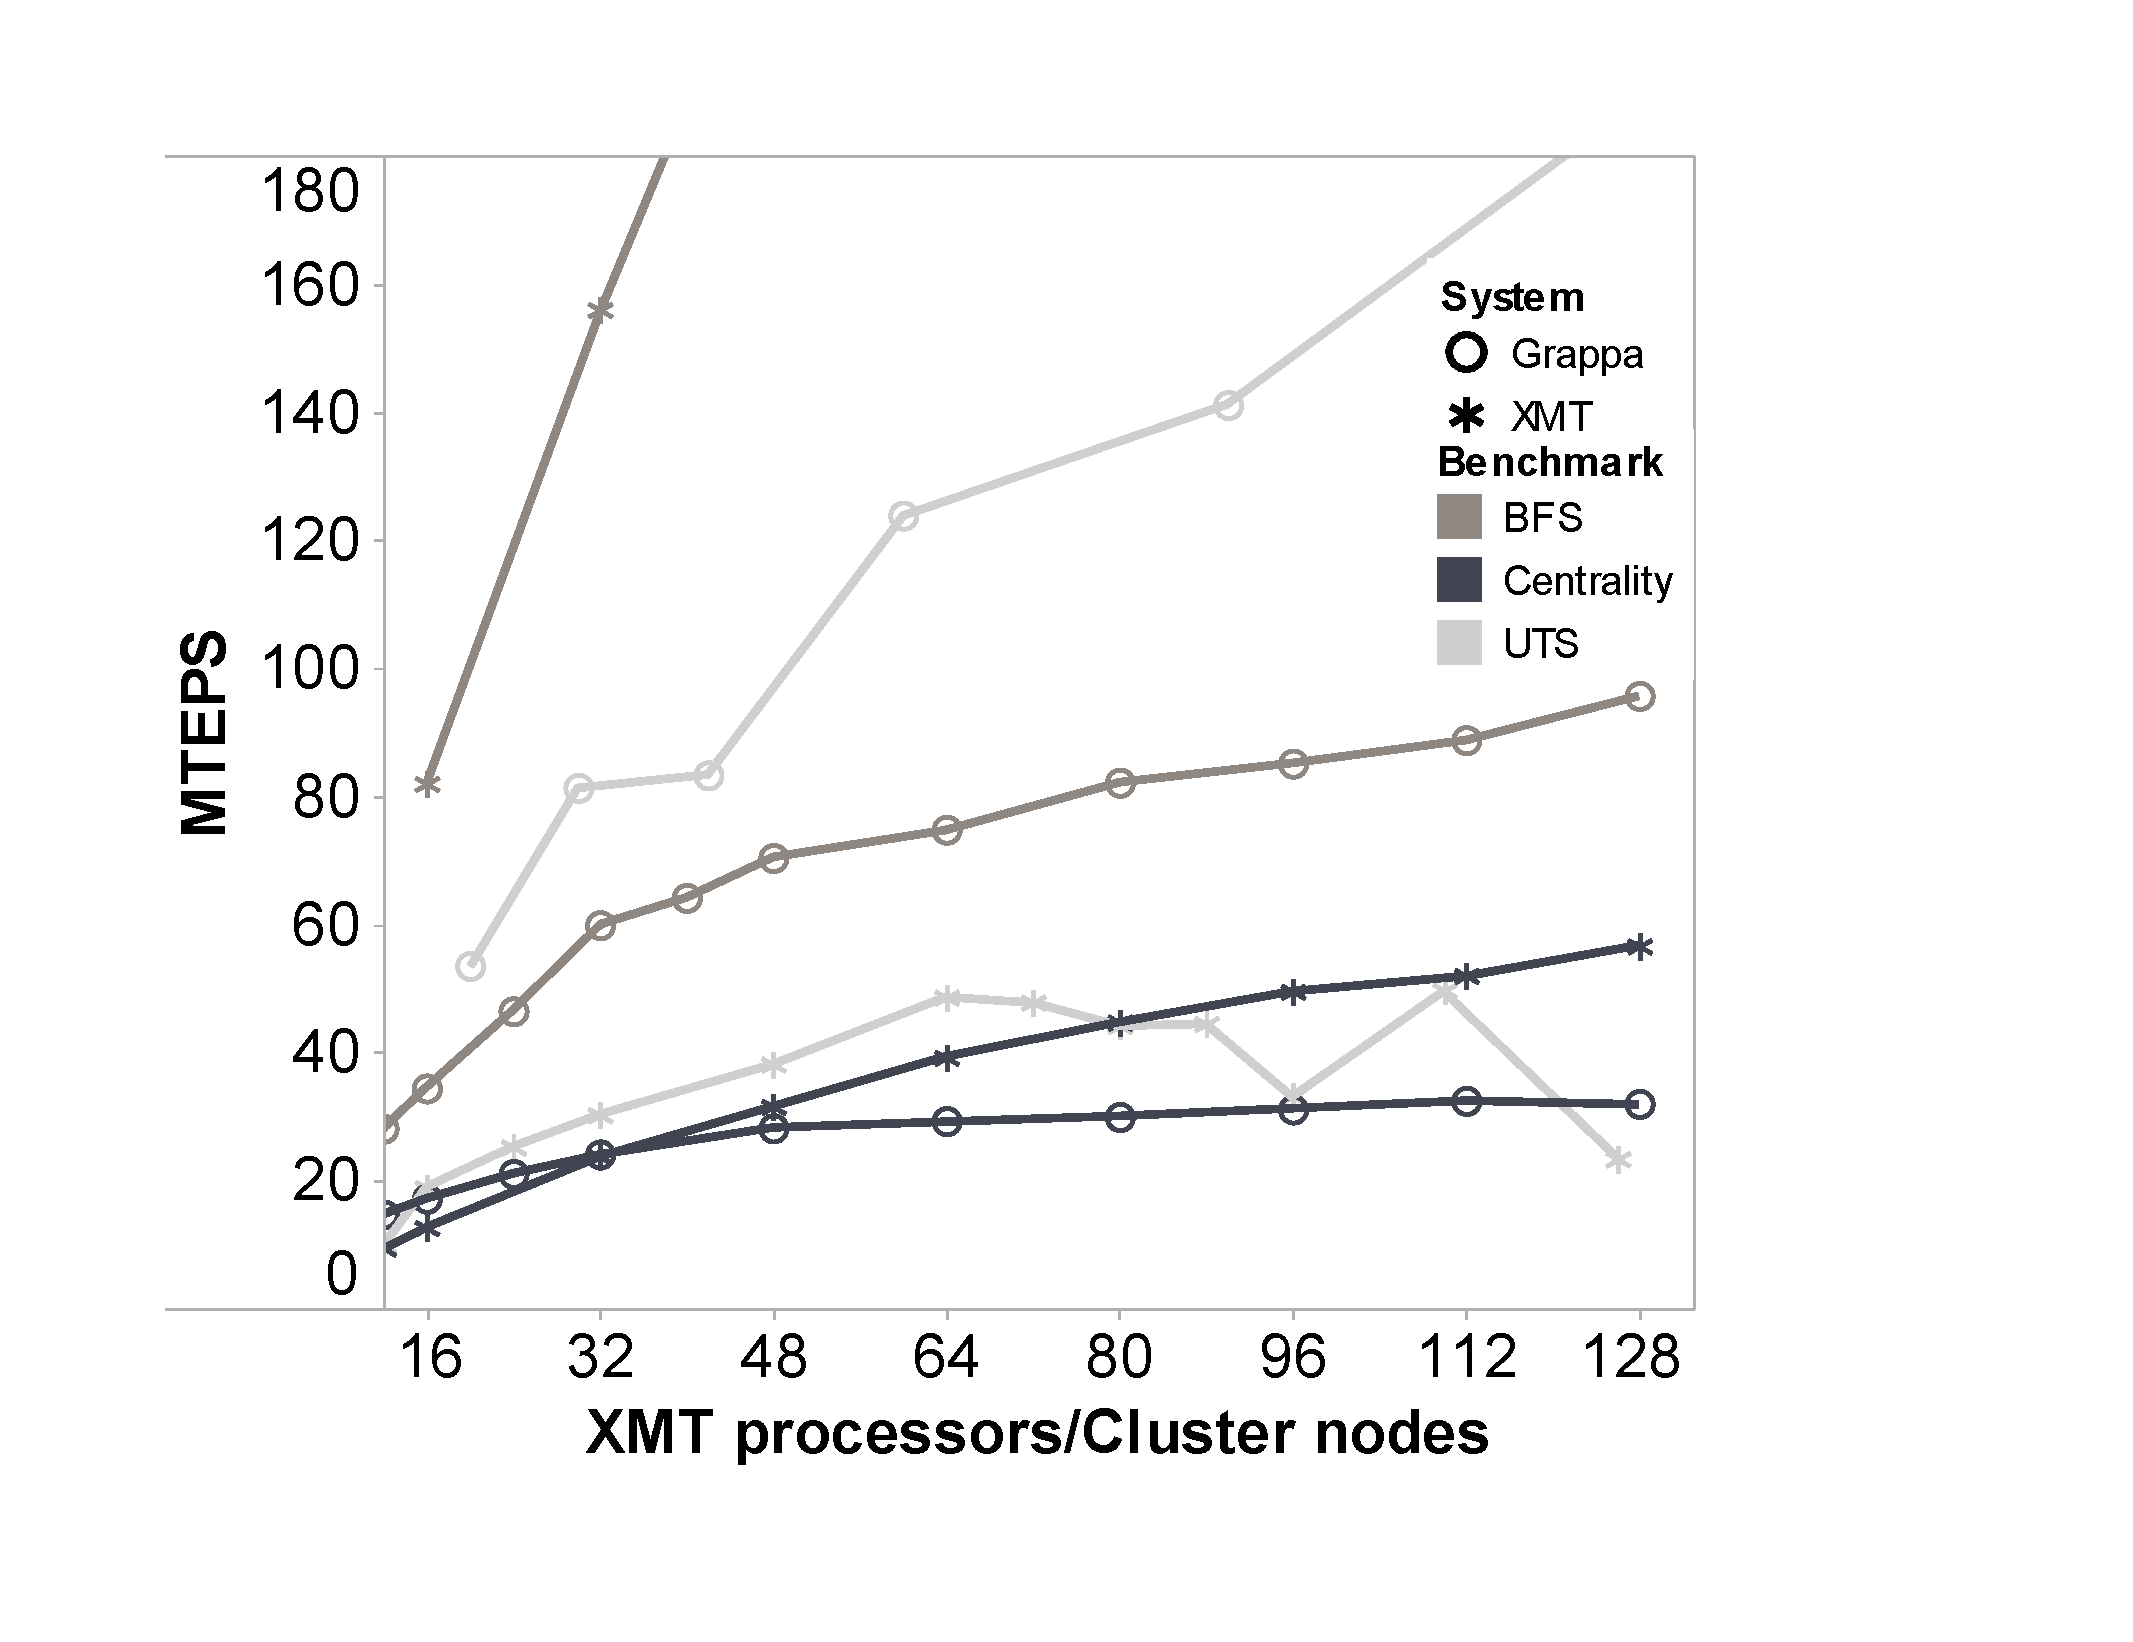
\includegraphics[width=0.5\textwidth]{figs/scaling_cropped.pdf}
    \end{center}
    \caption{Scaling number of nodes: \Grappa continues to perform significantly better than XMT for UTS but scales a constant factor slower than XMT for BFS (4x slower) and Centrality (2x slower). }
    \label{fig:uts_threshold}
\end{figure}

\subsection{Scaling}\label{sec:scaling} \TODO{rewrite with new results}

\subsubsection{Network Aggregation Performance and Robustness}

\begin{figure}[htb]
\begin{center}
  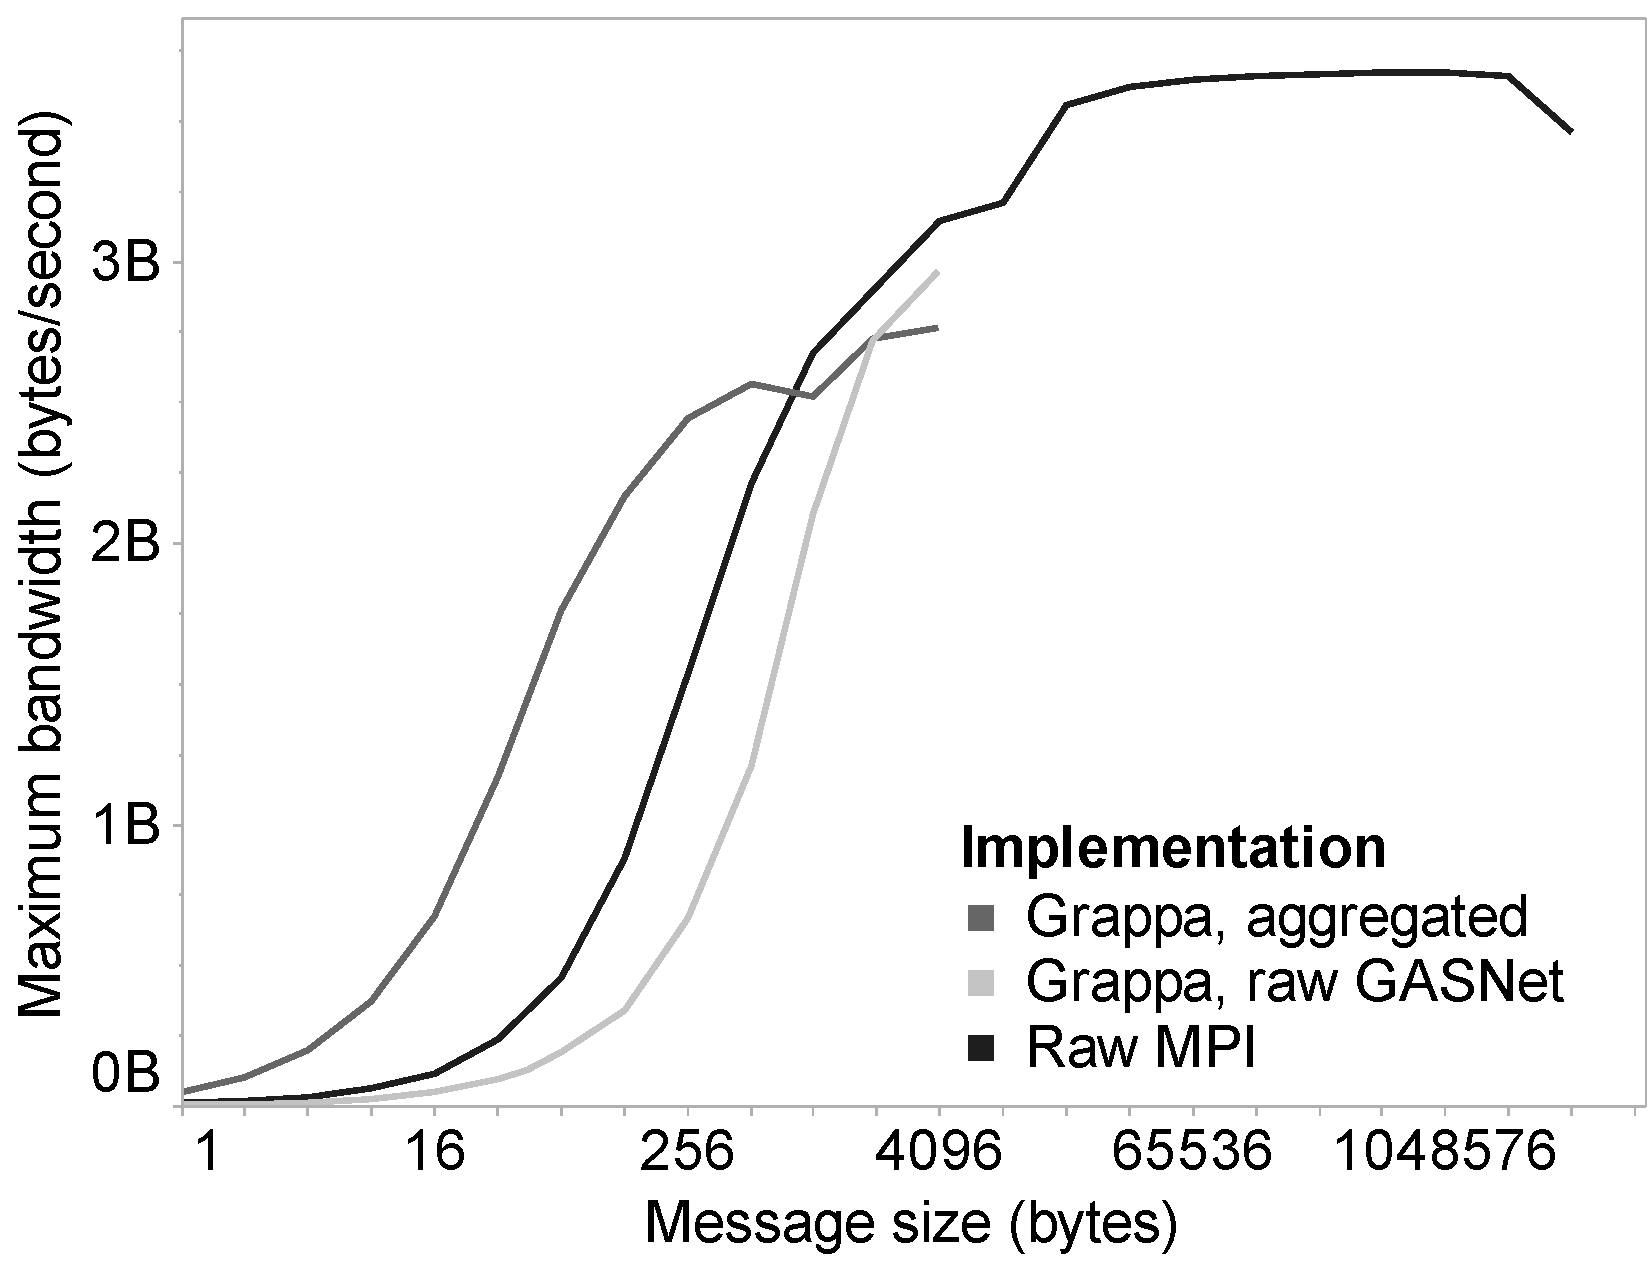
\includegraphics[width=0.95\columnwidth]{figs/aggregator_ping}
\begin{minipage}{0.95\columnwidth}
  \caption{\label{fig:aggregator-ping} Bandwidth versus message size
    unidirectional ping test for \Grappa with aggregation, \Grappa with
    raw GASNet messages, and MPI. Aggregation provides an 11x
    bandwidth benefit at our common operating point.}
\end{minipage}
\vspace{-3ex}
\end{center}
\end{figure}

To evaluate the benefits of network aggregation, we ran two experiments.
First, we ran a simple unidirectional ping test to see the maximum
benefit the aggregator can provide in terms of improved network
efficiency. Second, we ran BFS with the aggregator disabled in order to
measure its benefit on an application.

To implement the ping test, we wrote a simple \Grappa application where
the cores of one node send messages as fast as possible to the cores
of another node. We vary the size of the payload up the maximum
payload size supported by the aggregator (nearly 4KB). Each core has a
single task sending to a single destination, so this is a best case
scenario for the aggregator. To see the benefit of the aggregator, we
added a bypass that lets us send messages directly through GASNet. We
also compare against the OSU \texttt{osu\_mbw\_mr} benchmark
\cite{osu:mpi}  compiled against OpenMPI 1.5.3; this
benchmark has the same pattern of communication but doesn't have the
overhead of \Grappa's context switching.

The results are shown in Figure~\ref{fig:aggregator-ping}. There are
two key observations.

First, small message performance against the existing libraries is, as expected, poor. The MPI application test shows us that peak per node
bandwidth supported by our infiniband card is 3.4GB/s. This is
achievable only with large messages; we must send 16KB packets to get
within 5 percent of peak bandwidth. But in our benchmarks, we saw
average message between 32 and 64 bytes. At 32 bytes, the MPI test is
using less than 7 percent of its peak bandwidth. \Grappa sending
messages directly through GASNet uses less than 3 percent of the peak
bandwidth.

Second, aggregation has the potential to improve this situation by an
order of magnitude. With aggregation, \Grappa is able to send 32-byte
messages over 12 times faster than using GASNet directly. This is a
more respectable 32 percent of peak bandwidth. Due to expedient design
decisions, \Grappa's aggregator limits its aggregation to 4KB; this
limits its peak achievable bandwidth to 75 percent of the actual
peak.

This comparison is the best possible case for the aggregator. In
order to verify that the aggregator still has value on actual
applications at scale, we ran a small (100M node tree) UTS-Mem
with the aggregator disabled, on 16 nodes.
Figure~\ref{fig:no-aggregation-uts}. At this configuration, the aggregator
improves our application performance by 10x. 

\begin{figure}[htb]
\begin{center}
  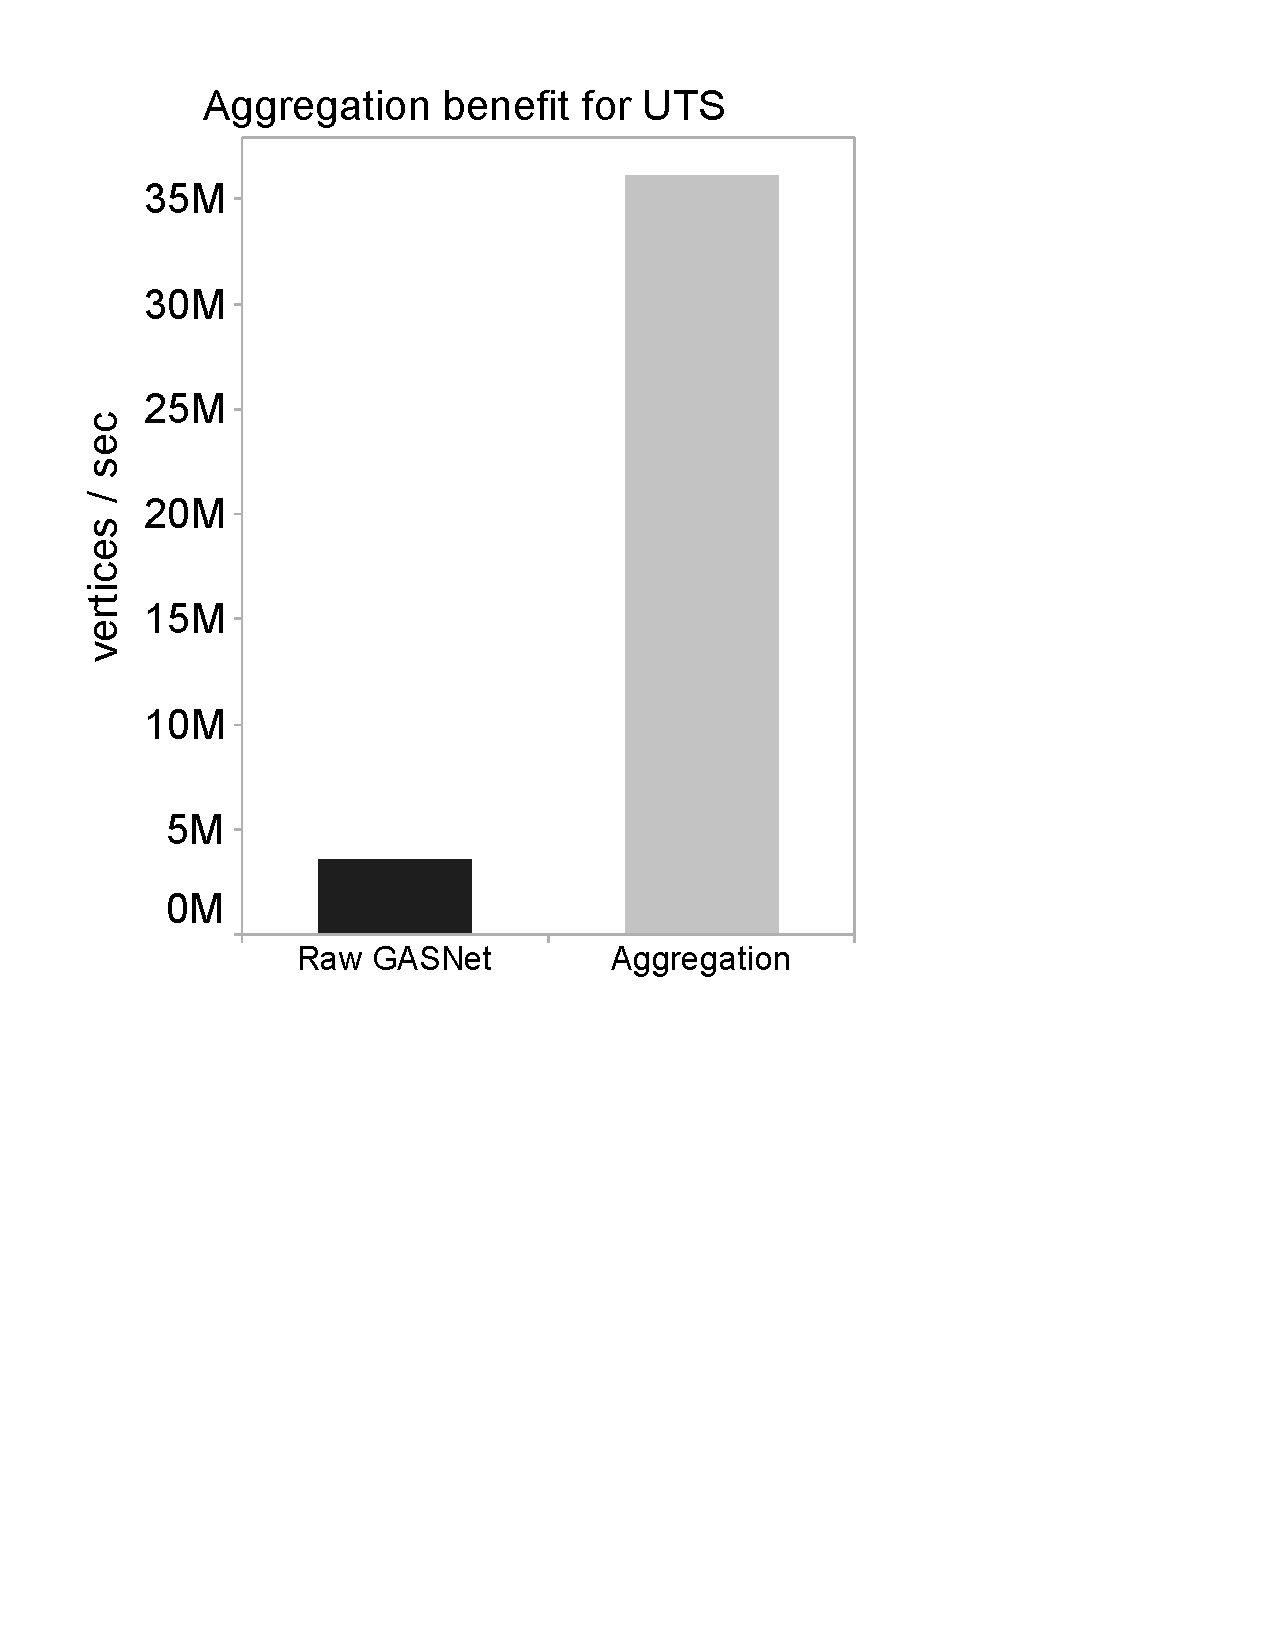
\includegraphics[width=0.95\columnwidth]{figs/no_aggregation_uts.pdf}
\begin{minipage}{0.95\columnwidth}
  \caption{\label{fig:no-aggregation-uts} Performance of UTS on 16
      nodes with and without \Grappa's aggregation.}
\end{minipage}
\vspace{-3ex}
\end{center}
\end{figure}

\subsection{Scaling}
% Got rid of this discussion of UTS by itself, tried to work the highlights in below
%\paragraph{UTS-Mem}
%We ran UTS-Mem on \Grappa and the XMT with a geometric 1.6B-vertex tree
%(T1XL) and a geometric 4.2B-vertex tree (T1XXL), using up to 128
%nodes---the maximum we had available for each. \Grappa results are for 5 cores per node. \Grappa with 20 machines is faster than the entire XMT of 128 processors.
%\Grappa achieves \checkme{188Mvert/s} with 128 nodes and the XMT
%achieves only 50Mvert/s, plateauing at 60 nodes. Beyond 90 nodes, \Grappa adds 1.4 Mvert/s/node.
%The XMT scales at 850 Kvert/s/node, until it plateaus. \Grappa keeps
%scaling up through 128 nodes, although scaling
%declines because of the unscalability of our aggregation mechanism as
%number of network endpoints increases. 
%
%Despite our efforts to tune the UTS implementation specific to the 
%XMT, performance does not scale well with increasing processor count,
%flattening out around 60 processors.  When we increase the size of
%the tree from 100M to 4.2B, we find that performance does not improve,
%suggesting that performance is not limited by task parallelism.
%Cray's performance tools show an increasing number of memory
%retry operations for failed synchronization operations generated by
%the runtime, which create network contention.
%
To determine how \Grappa's performance scales compared to the performance of the entire XMT, we ran a set of experiments up to all 128 XMT processors and 128 cluster nodes. For the XMT, the number of allowed processors was varied up to the entire machine, with some minor tuning of stream parameters needed to get optimal performance. For \Grappa, parameters such as cores per node, aggregator timeouts, and parallel threshold were tuned to get the best performance for each node count. All of the benchmarks continue to improve out to 128 nodes for \Grappa. UTS continues to fare better than the XMT with large node counts, with the XMT appearing to plateau at 60 processors due to contention from synchronization retries, while \Grappa handles this by suspending tasks until messages return. For BFS and Centrality, the XMT scales approximately a constant factor better than \Grappa. We attribute this to a limitation in the current aggregator design and network stack that \Grappa uses.  This limits the practical number of cores we can use to 6 per node (adding more cores per node \emph{decreases\/} performance).  Ironically, this limitation makes \Grappa applications compute-bound instead of network-bound.  Work is ongoing to rework the Infiniband driver stack and aggregation interface to remove this limitation and improve aggregation addressing using local routing.

\begin{figure}[ht]
    \begin{center}
      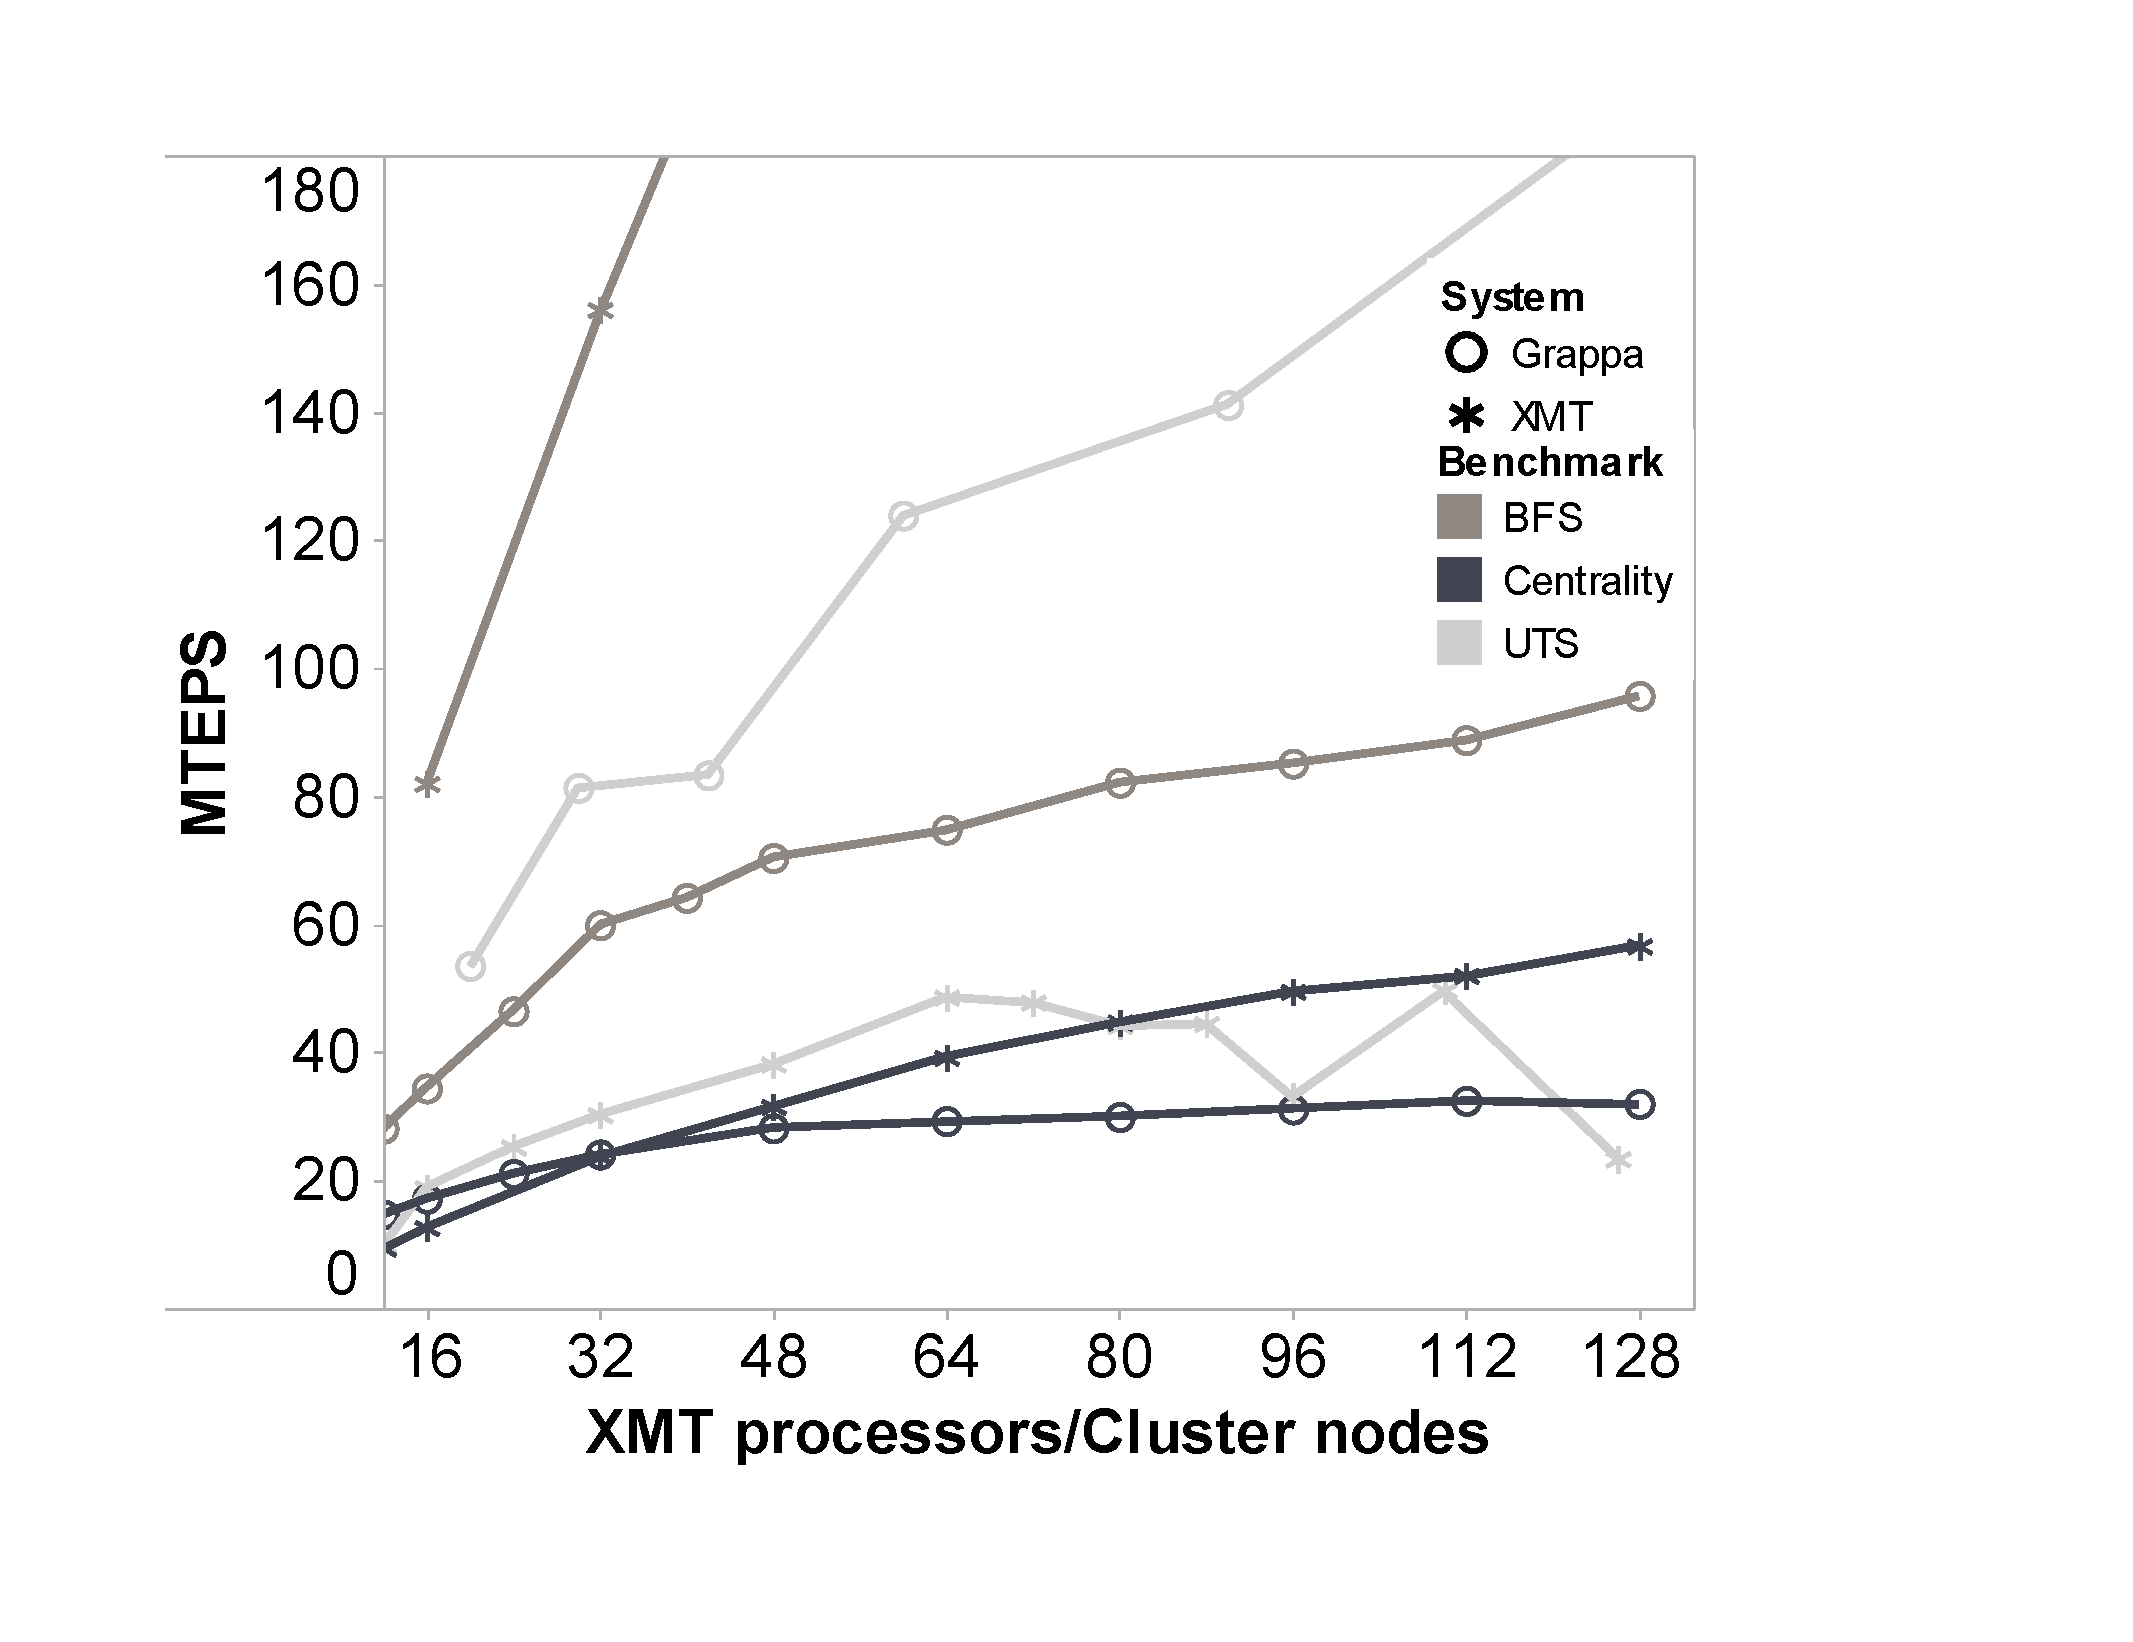
\includegraphics[width=0.5\textwidth]{figs/scaling_cropped.pdf}
    \end{center}
    \caption{Scaling number of nodes: \Grappa continues to perform significantly better than XMT for UTS but scales a constant factor slower than XMT for BFS (4x slower) and Centrality (2x slower). }
    \label{fig:uts_threshold}
\end{figure}


\subsection{Sensitivity}

\paragraph{Aggregator timeout}

\begin{figure}[htb]
\begin{center}
  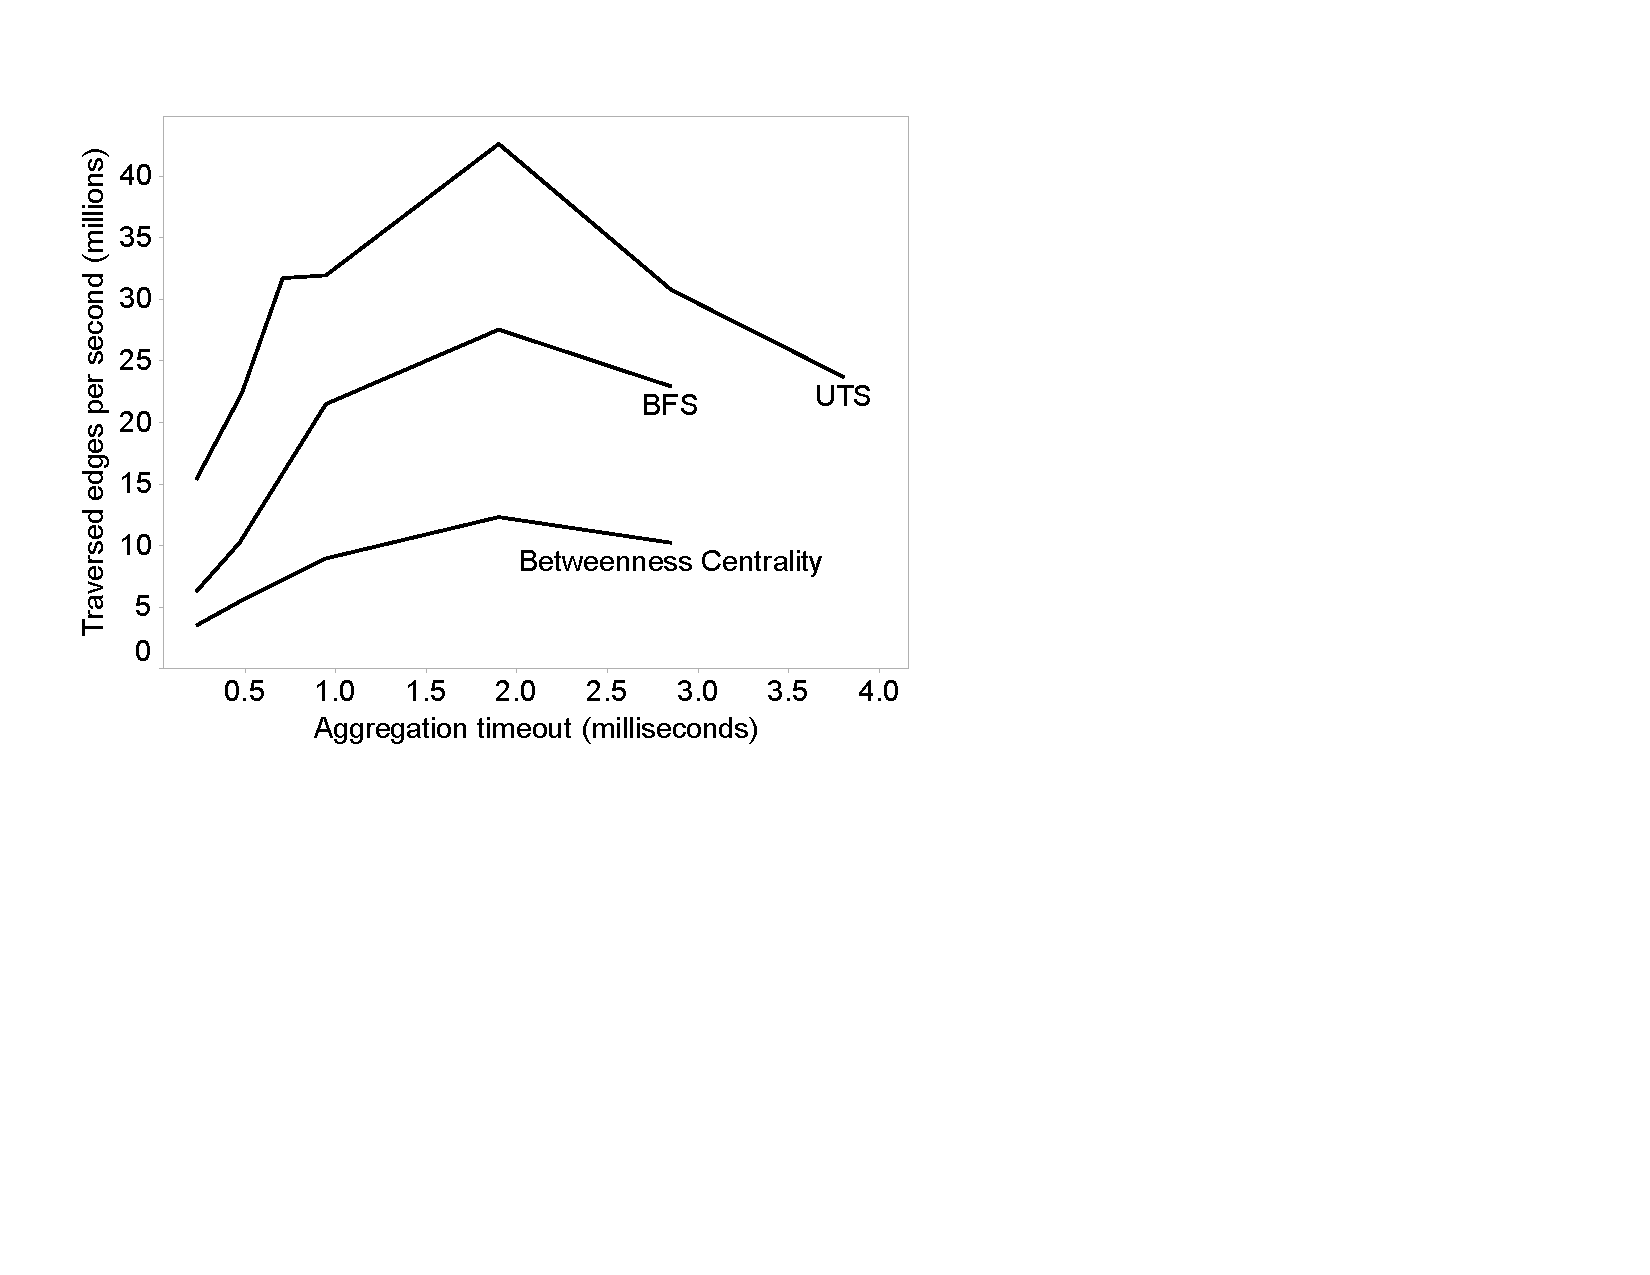
\includegraphics[width=0.95\columnwidth]{figs/flushticks_sweep}
\begin{minipage}{0.95\columnwidth}
  \caption{\label{fig:bfs-sweep-flushticks} Sensitivity to aggregation delay}
\end{minipage}
\vspace{-3ex}
\end{center}
\end{figure}


One of the key parameters of the aggregator is the message
timeout. All messages that are queued must eventually be sent in order
to ensure progress. In the best case, we are able to aggregate enough
messages to fill an aggregation buffer and cause it to be sent, but as
we scale up, the average rate of messages heading to a common
destination decreases, and this gets harder. To bound the problem, the
aggregator includes a timeout. Any packet waiting this long is sent
the next time the communications layer is serviced.

Figure~\ref{fig:bfs-sweep-flushticks} shows a sweep of this parameter
for UTS, BFS, and Betweenness Centrality on 16 nodes, using the
datasets described previously. The maximum number of workers is fixed
at 2048. All the benchmarks show a performance peak with a 2
millisecond timeout; at this point we are delaying long enough to
aggregate the largest packets we can; setting the parameter higher
causes tasks to wait longer for responses, but few new requests are
being generated.


\begin{figure}[htb]
\begin{center}
  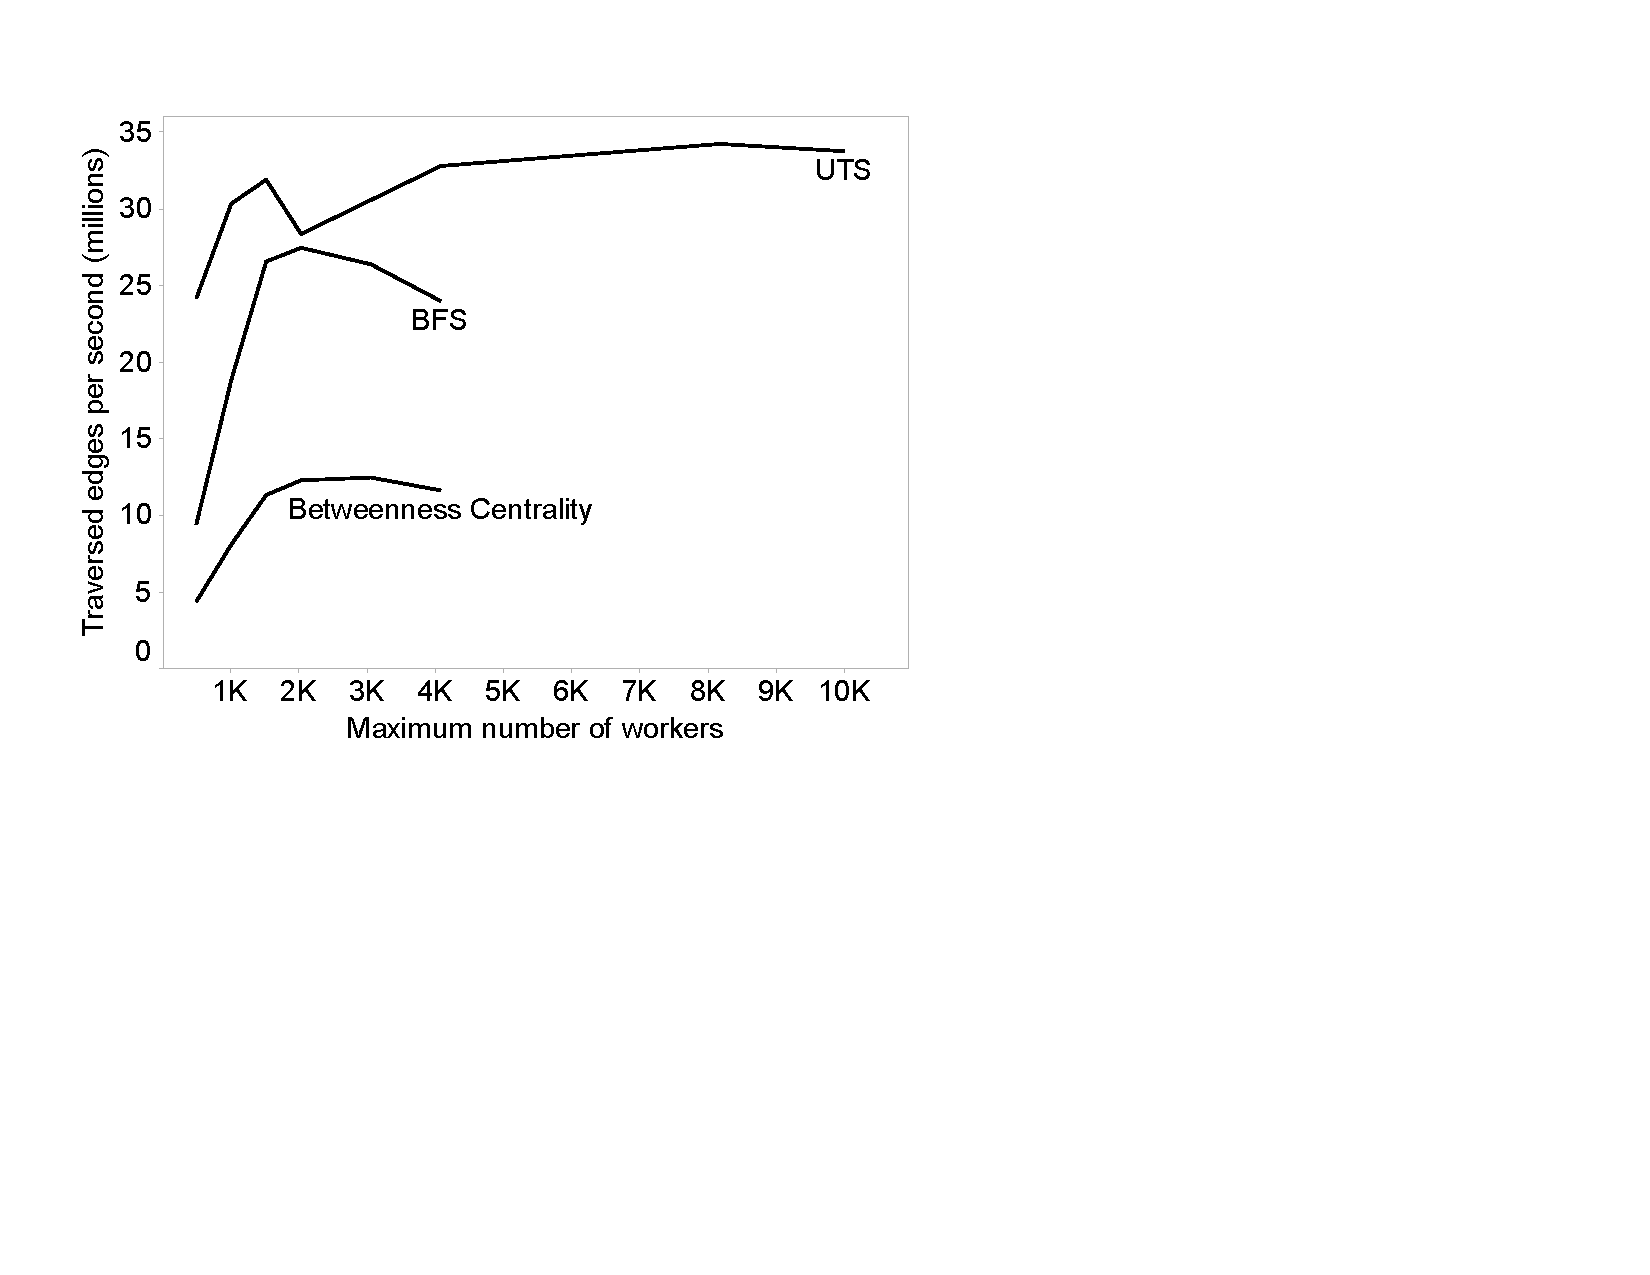
\includegraphics[width=0.95\columnwidth]{figs/worker_sweep}
\begin{minipage}{0.95\columnwidth} 
  \caption{\label{fig:bfs-sweep-workers} Sensitivity to maximum active tasks}
\end{minipage}
\vspace{-3ex}
\end{center}
\end{figure}

\subsubsection{Number of active tasks} \TODO{possibly eliminate}

When a task issues a request that requires a response, it blocks to
allow other tasks to utilize its core. These tasks may also block. To
support the many milliseconds of latency aggregation adds, we need to
support many thousands of blocked tasks. One of the key parameters of
the runtime is the number of blocked tasks allowed; we need enough to
cover the network and aggregation latency, but too many running tasks
can add extra latency as they all must be multiplexed onto the same core.

Figure~\ref{fig:bfs-sweep-workers} shows a sweep of the maximum number
of active tasks (workers) per core for each of our three benchmarks on
16 nodes. The aggregator timeout is set at 1 ms for UTS and 2 ms for
BFS and Betweenness Centrality. The performance peak shifts in this
case, with UTS peaking at 1536 workers, BFS peaking at 2048 workers,
and Betweenness Centrality peaking at 3072 workers. This is the point
where we have enough workers to cover the latency of aggreation. The
different values reflect the different amounts of work done by a task
in each benchmark; UTS does the least, while Betweenness Centrality does the most.

%\subsubsection{Work stealing parameters}
%
%\paragraph{Chunk size}
%
%It is important to steal multiple tasks at a time to both amortize the
%cost of stealing over the network and to spread out work quickly in a
%large system. Figure~\ref{fig:ut_chunksize} shows performance and
%stealing statistics for UTS on \checkme{30} nodes as we increase the stealing chunk size. Recall
%that a thief will take a number of tasks equal to the minimum of half
%the available work or the chunk size; steals fail only when the victim
%has fewer than 2 available tasks. As the scheduler is allowed to
%steal more work beyond 1 task, we see that performance increases up to 6x. This
%shows that the heuristic of stealing the oldest task from victims is
%insufficient alone when a tree-structured computation is imbalanced,
%as observed in \cite{UTS}. By observing sampled state in the execution
%trace, we find that a chunk size as low as 1 allows stealing to
%spread the load evenly across the cluster but cores spend much time
%underutilized as multiple workers wait for steal replies that
%utlimately return little new work.
%
%Performance plateaus before maximum steal amount is limited by the
%size of the victim's task queue. This indicates that artificially limiting steals
%to \checkme{128} tasks does not limit performance. Although a lower
%chunk size limits how quickly work spreads, for sufficient chunk size,
%the heuristic of stealing the oldest tasks from victims in tree-based computations allows for
%stolen work to expand quickly.


%% UTS: chunk size
%\begin{figure}[ht]
%    \begin{center}
%      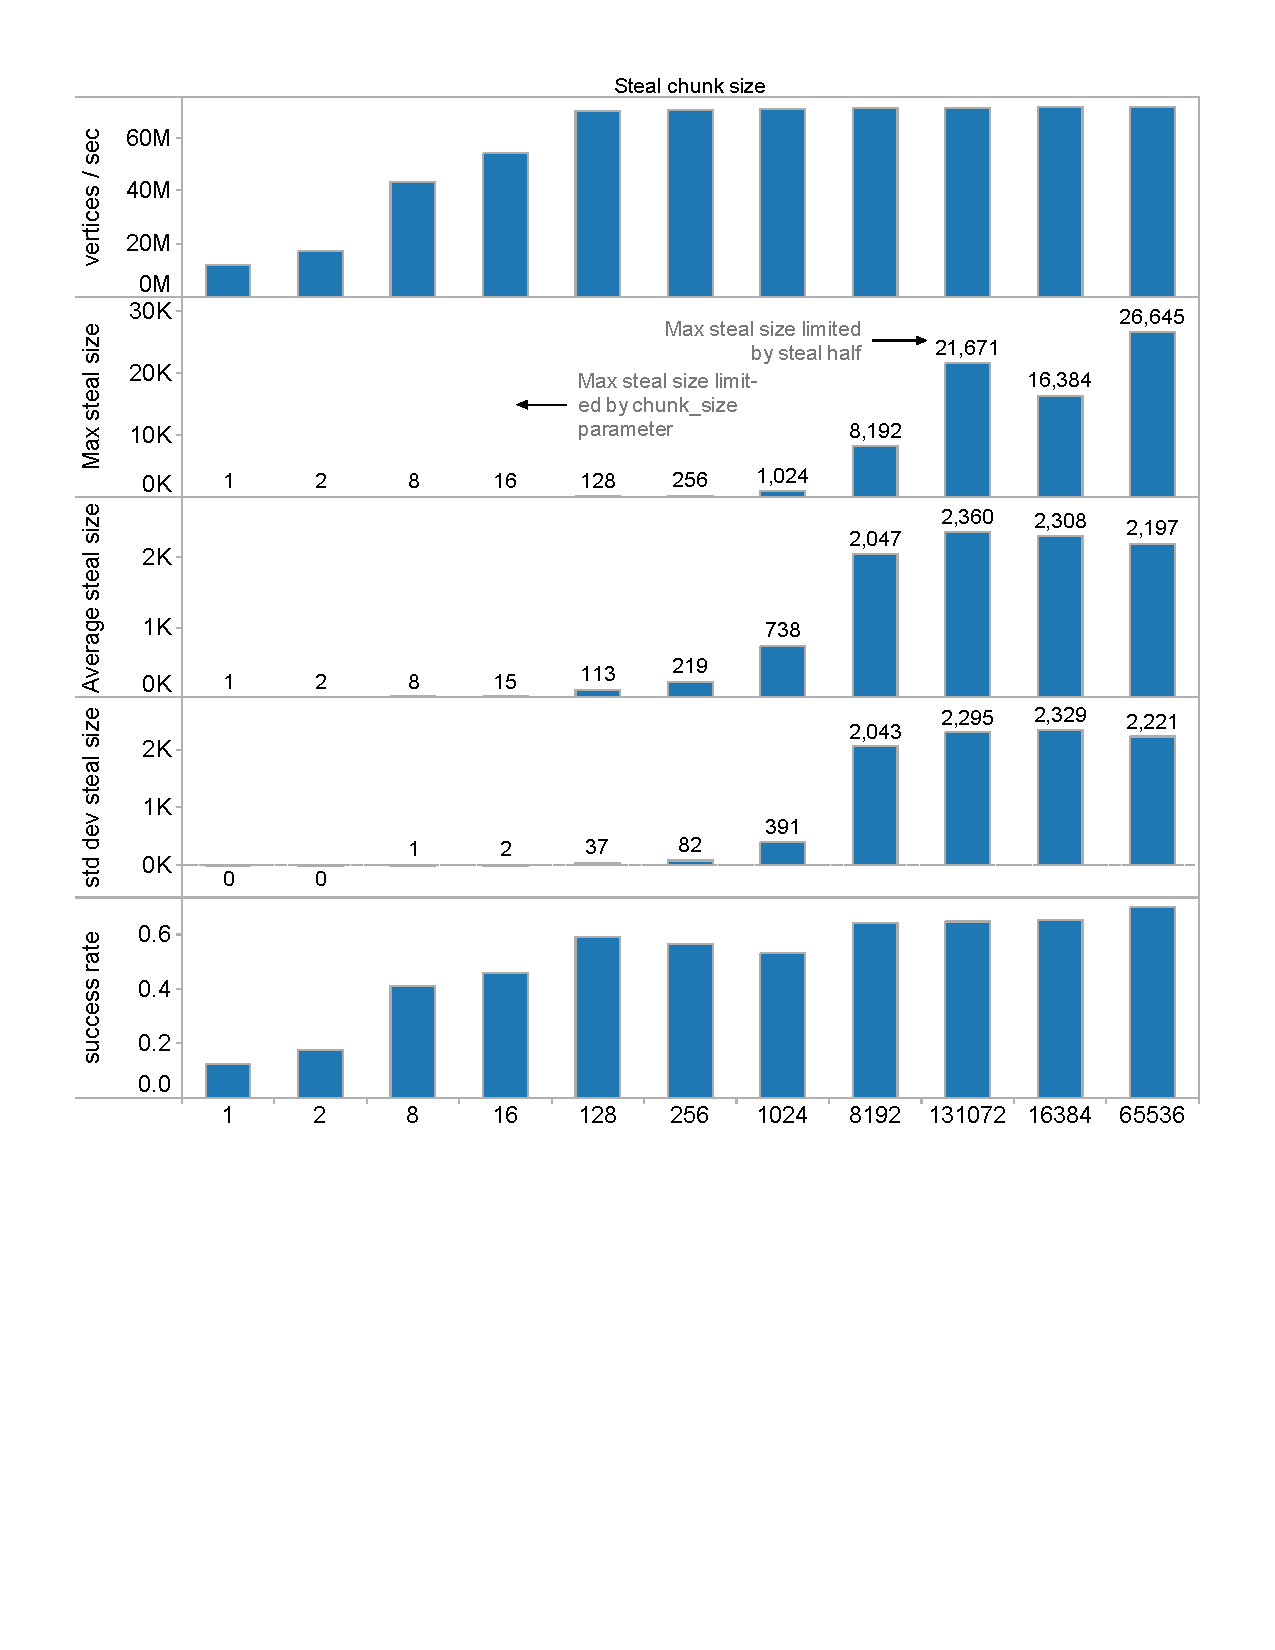
\includegraphics[width=0.5\textwidth]{figs/uts_chunksize.pdf}
%    \end{center}
%    \caption{Performance of UTS-Mem with varying maximum chunk size of
%    steals, run with 30 nodes, 6 cores per node, 4000 workers,
%    \checkme{6M flush ticks}}
%    \label{fig:uts_chunksize}
%\end{figure}


%\TODO{(difference with BFS)}



\subsubsection{Parallel loop threshold}

%\begin{figure}[htb]
%\begin{center}
%  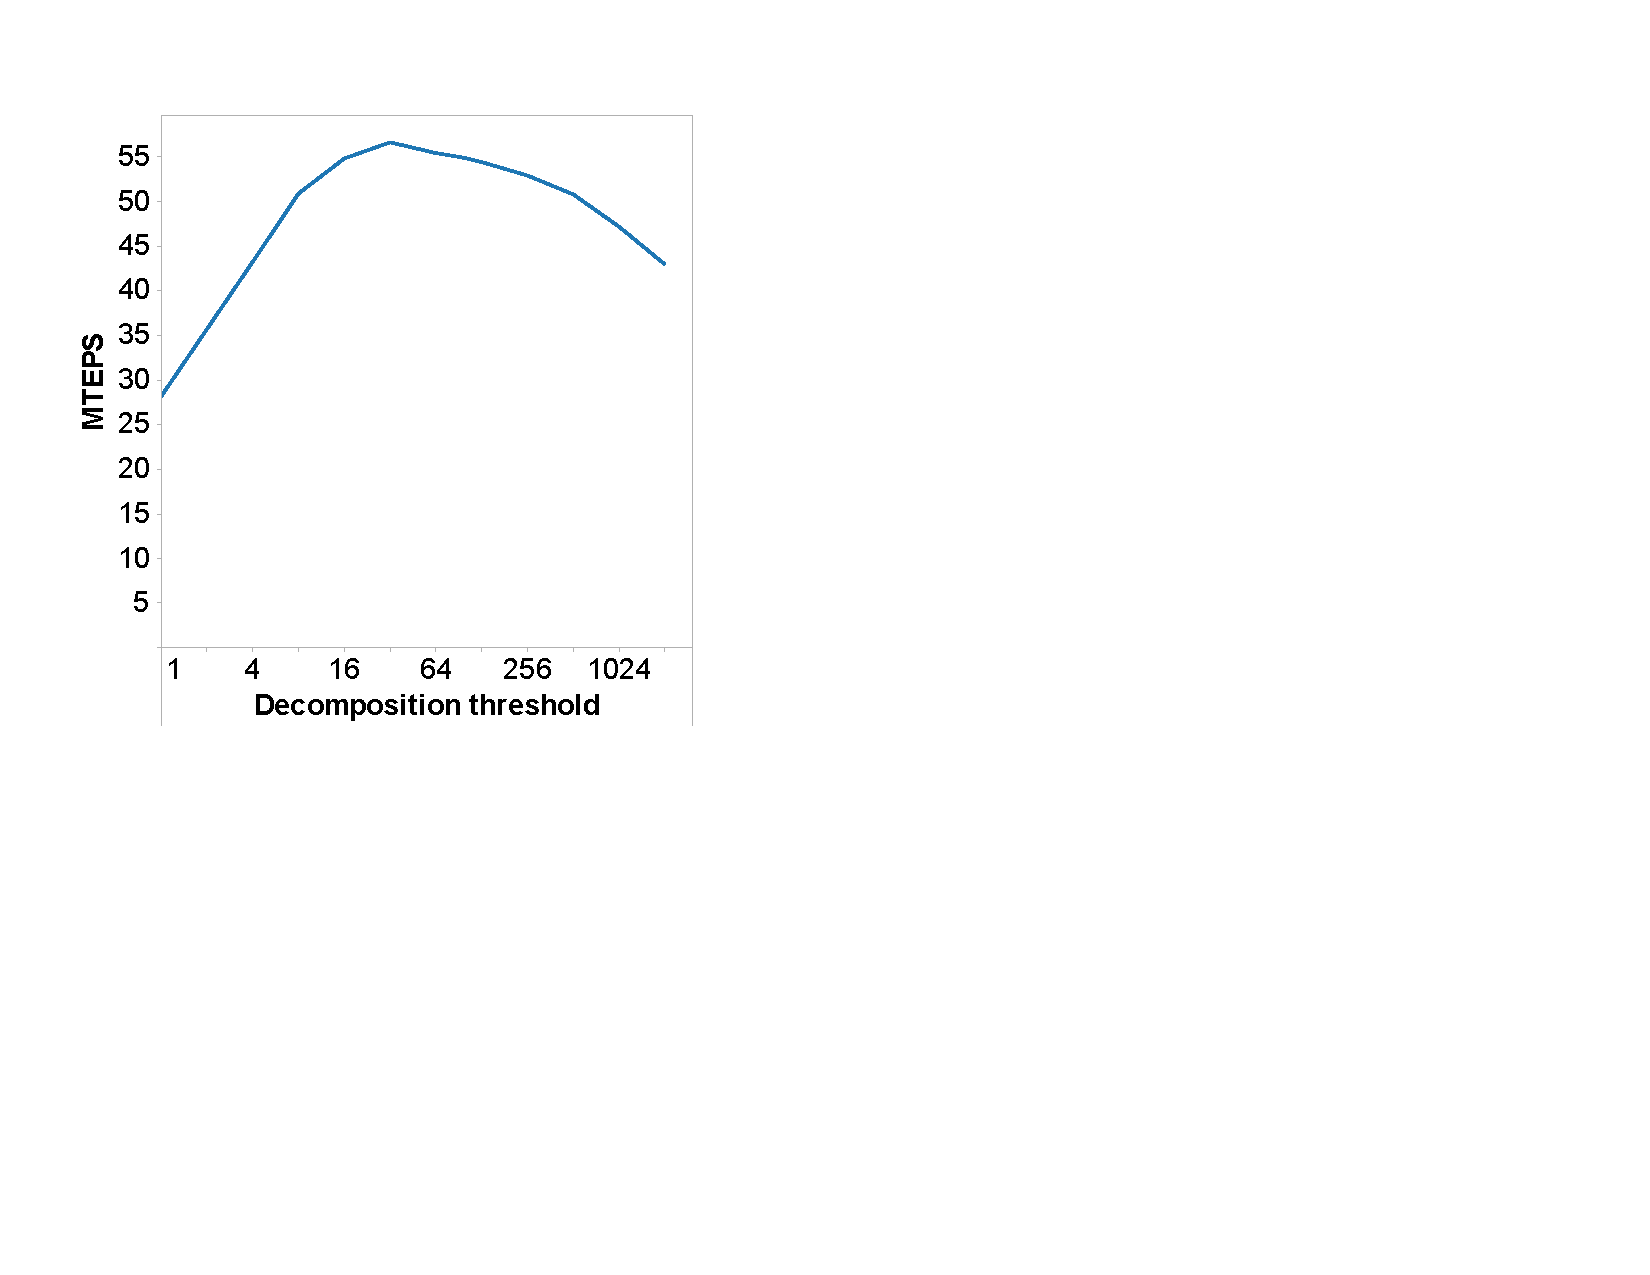
\includegraphics[width=0.95\columnwidth]{figs/bfs_sweep_threshold}
%\begin{minipage}{0.95\columnwidth}
%  \caption{\label{fig:bfs-sweep-threshold} Sensitivity to parallel loop threshold. Note the log scale.}
%\end{minipage}
%\vspace{-3ex}
%\end{center}
%\end{figure}

Parallel overhead---in the form of context switches, task spawns, and
synchronization---can reduce the performance benefit of parallelism.
\Grappa sees a benefit to limiting the amount of parallelism created by
a recursive loop decomposition. The parallel loop threshold (``parallel
granularity'') parameter tells the runtime when to stop creating new tasks and just execute iterations
sequentially. This allows us to amortize the overhead of task
creation. In addition, assigning sequential iterations to a single
task provides the potential to exploit locality when data for adjacent iterations is
also adjacent in memory. The ability to exploit this locality that
exists in the application is an important advantage. We found that in UTS and BFS, increasing the
threshold from 1 up to 8 or 16, respectively, increases performance by
more than 60\%.


% uts threshold
%\begin{figure}[ht]
%    \begin{center}
%      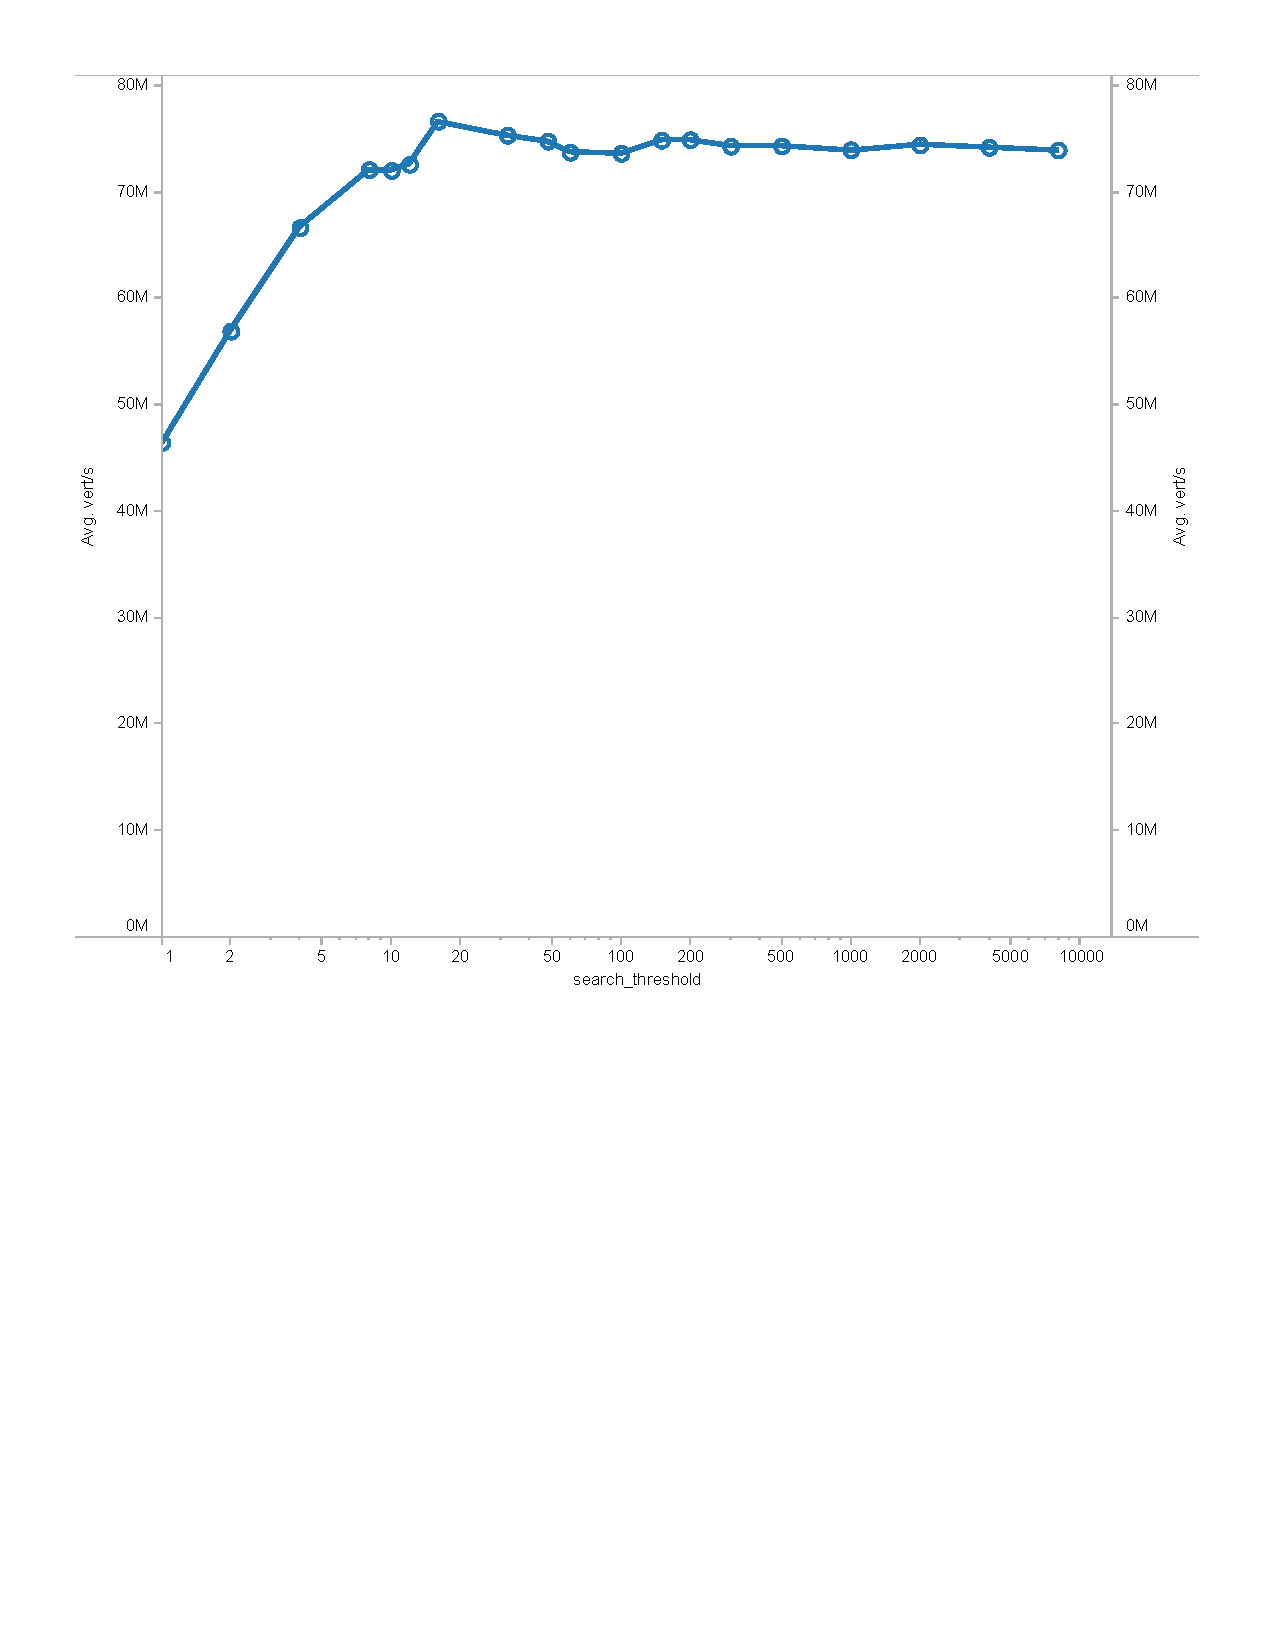
\includegraphics[width=0.5\textwidth]{figs/uts_threshold.pdf}
%    \end{center}
%    \caption{Performance of UTS-Mem with varying parallel loop
%        threshold, run with 30 nodes, 6 cores per node, 4000 workers,
%    \checkme{6M flush ticks}}
%    \label{fig:uts_threshold}
%\end{figure}

\subsection{Summary}\TODO{this is a placeholder: do we need this section?}

\paragraph{Context-switch overhead.} Should we also compare with other packages? (Maybe Capriccio, QThreads?, or even real OS threads?)

\paragraph{Latency.} Measure remote data access latency with and without aggregation turned on.

\paragraph{Aggregated message sizes.} Characterization of the resulting message sizes with aggregation. Right now we only have message size vs. bandwidth.

\paragraph{Utilization.} CPU utilization, Memory, Network. It would be great to answer the question of where is our bottleneck right now. Amount of concurrency with and without aggregation. 

\paragraph{Memory accesses.} Rate of accesses to remote data. Rate of delegate ops. Show limit with GUPs.



%Retries are performed by the memory controller when remote synchronization operations fail to find the full-bit associated with each memory location in the unavailable state.  Retries are issued at low priority relative to new memory operations issued by the processor by other contexts, so they consume what would otherwise be unused injection bandwidth.  On a full-bandwidth system such as the MTA-2, retries have no impact on the progress of tasks other than their own.  On a Cray XMT, network bandwidth is limited, so retries create congestion.  In comparison, \Grappa performs synchronization without retries, delaying responses at the receiving end until ready to notify the sender to proceed.  This saves bandwidth and permits scaling of tasks performing synchronization even on low injection rate networks.


%\begin{figure*}[ht]
%    \begin{minipage}{0.3\linewidth}
%        \centering
%        \includegraphics[width=\textwidth]{figs/chunksize-uts.pdf}
%        \caption{chunksize caption}
%        \label{fig:chunksize-uts}
%    \end{minipage}
%    \begin{minipage}{0.3\linewidth}
%        \centering
%        \includegraphics[width=\textwidth]{figs/workers-uts.pdf}
%        \caption{workers caption}
%        \label{fig:workers-uts}
%    \end{minipage}
%    \begin{minipage}{0.3\linewidth}
%        \centering
%        \includegraphics[width=\textwidth]{figs/thresh-uts.pdf}
%        \caption{threshold caption}
%        \label{fig:thresh-uts}
%    \end{minipage}
%\end{figure*}

}

%\todo{End eval insert}

\section{Related work}
\label{sec:related}
The concept of using independent parallel contexts to tolerate latency
is not novel.  The inspiration for our project is of course the Cray
XMT \cite{feo-xmt}, which implemented a hardware version of our
programming model (in what would today be considered exceptionally
slow silicon.)  The XMT can be seen as simultaneous multithreading
\cite{tullsen-smt} writ large; the technique and motivation is
essentially the same, but the XMT allows hundreds of contexts (modern
Intel SMT implementations are generally limited to two.) The Alewife
system \cite{agarwal-alewife} also switches contexts (in hardware) to
hide latency on remote-node accesses.  Cyclops \cite{almasi-cyclops}
allows hundreds of independently executing contexts to share FPUs,
caches, and paths to memory, but does not context switch or share
basic execution hardware.  

Modern programmable GPUs, such as nVidia's CUDA programming model, can also be interpreted in using an XMT-like
model under the hood;
% Do I need to include a citation here?
while they generate large numbers of available execution contexts via
a (semi-)explicit SIMD model, those SIMD instructions keep functional
units satisfied by overlapping execution with the loads required for
other contexts.

Similar techniques have also been used in software.  Mowry proposed a system \cite{mowry-scm} of \emph{software-controlled
  multithreading}.  As opposed to our system of explicitly marked
remote references, SCM assumes a high hit rate and traps to an
interrupt routine which performed a context switch upon a cache miss.  The 2000-era processors had
short enough latencies that using more than two contexts generally
produced slowdown.

Partitioned global address space models, such as that used in Unified Parallel C,
% definitely need a citation here
 share our approach of exposing all data (even remote data)
 transparently to any threads and have largely solved the problems of
 how to efficiently translate those remote reads into message
 passing.  However, their programming models emphasize locality more
 than our work does; while a program can examine any vertex in a UPC
 program at any time, it probably shouldn't (whereas our kernels rely on our
 latency hiding technique to make common remote references fast.

The value of the information in extremely large and sparse graphs is
rapidly growing.  The GraphCT toolkit \cite{ediger-graphct} used an XMT to perform
sophisticated analysis on data from Twitter, identifying important
actors and their networks of influence, and it can scale to the full
size of graphs such as Facebook's friend network.

\section{Conclusion}
\label{sec:conclusion}


\bibliographystyle{acm}
\bibliography{softxmt-hotpar2011}

\end{document}
